\PassOptionsToPackage{hyperfootnotes=false}{hyperref}
\documentclass[a4paper,fleqn]{cas-sc}
\renewcommand{\sfdefault}{lmss}
\renewcommand{\ttdefault}{lmtt}

\usepackage[numbers]{natbib}
\usepackage[version=4]{mhchem}
\usepackage{cleveref}
\usepackage{mathtools}
\usepackage{amssymb}
\usepackage{tabularx}
\usepackage{makecell}
\usepackage{booktabs}
\usepackage{longtable}
\usepackage{pdflscape}
\let\articlecaption\caption
\usepackage{algorithm}
\let\algorithmcaption\caption
\let\caption\articlecaption
\AtBeginEnvironment{algorithm}{\small\let\caption\algorithmcaption}
\usepackage{algpseudocode}
\usepackage{xspace}
\usepackage{xcolor}
\usepackage{siunitx}
\usepackage{xurl}
\usepackage{listings}
\usepackage{tikz}
\usetikzlibrary{arrows.meta,positioning,fit,backgrounds,calc}
\usepackage{pgfplots}
\pgfplotsset{compat=1.18}
% CSE semantic figure styles. Load after tikz and pgfplots.
\definecolor{cseBlue}{HTML}{0072B2}
\definecolor{cseOrange}{HTML}{D55E00}
\definecolor{cseGreen}{HTML}{009E73}
\definecolor{csePurple}{HTML}{CC79A7}
\definecolor{cseGold}{HTML}{E69F00}
\definecolor{cseSky}{HTML}{56B4E9}

\tikzset{
  cse node/.style={
    draw,
    rounded corners=2pt,
    align=center,
    minimum width=25mm,
    minimum height=9mm,
    inner sep=3pt,
  },
  cse arrow/.style={-{Latex[length=2mm]}, thick},
  cse panel frame/.style={
    draw=cseSky,
    fill=cseSky!7,
    rounded corners=2pt,
    inner sep=3mm,
  },
  cse panel caption/.style={font=\scriptsize, align=center},
}

\pgfplotsset{
  cse axis/.style={
    width=0.86\linewidth,
    grid=both,
    tick align=outside,
    legend style={draw=none, fill=none},
  },
  cse model/.style={very thick, cseBlue, no marks},
  cse data/.style={only marks, mark=o, mark size=2.2pt, cseOrange},
  cse reference/.style={only marks, mark=x, mark size=2.5pt, cseGreen},
  cse uncertainty/.style={draw=none, fill=cseSky, fill opacity=0.24},
}

\graphicspath{{figures/generated/}}

\newcommand{\code}[1]{\texttt{#1}}
\newcommand{\COtwo}{\ce{CO2}\xspace}
\newcommand{\ares}{a^{\mathrm{res}}}
\newcommand{\todo}[1]{\textcolor{red!60!black}{[\textbf{TODO:} #1]}}
\newcommand{\figplaceholder}[2]{\begin{center}\fbox{\parbox[c][#1][c]{0.9\linewidth}{\centering\textcolor{black!65}{\textit{Planned figure:} #2}}}\end{center}}
\lstset{language=Python,basicstyle=\ttfamily\footnotesize,columns=fullflexible,keepspaces=true,frame=lines,commentstyle=\color{black!60},showstringspaces=false}

\begin{document}

\let\WriteBookmarks\relax
\renewcommand{\lastpage}{\csname @abspage@last\endcsname}
\renewcommand{\topfraction}{0.95}
\renewcommand{\bottomfraction}{0.8}
\renewcommand{\textfraction}{0.07}
\renewcommand{\floatpagefraction}{0.8}

\shorttitle{ePC-SAFT: exact-derivative electrolyte equation-of-state engine}
\shortauthors{Polley}

\title[mode = title]{\texorpdfstring{ePC-SAFT: an electrolyte equation-of-state engine with exact derivatives for phase and reaction equilibrium and parameter estimation}{ePC-SAFT: an electrolyte equation-of-state engine with exact derivatives for phase and reaction equilibrium and parameter estimation}}

\author[1]{Tanner W. Polley}[orcid=0009-0008-5957-4152]
\cormark[1]
\ead{tpolley3@byu.edu}

\affiliation[1]{
    organization={Department of Chemical Engineering, Brigham Young University},
    city={Provo},
    state={UT},
    postcode={84602},
    country={United States}
}

\cortext[cor1]{Corresponding author.}

\begin{abstract}
% P:abstract-01
Electrolyte parameter estimation and equation-oriented process models require properties of a solved phase and reaction equilibrium and their responses to temperature, pressure, feed and molecular parameters.
The ePC-SAFT package supplies these calculations in native C++ through a Python interface.
Published hard-chain, dispersion, association, polar and electrolyte contributions define a selected Helmholtz energy; association and pressure closure, constrained equilibrium and exact derivatives share its mathematical implementation.
One equilibrium driver handles declared neutral, charged and reacting phase specifications, while explicit tangent-plane searches test additional phases.
Implicit derivatives of the defining equations supply observation Jacobians, least-squares and guarded minimax parameter estimation, and first and second derivatives for process models.
Comparisons span pure-fluid saturation, neutral and associating mixtures, aqueous and mixed electrolytes, solvent transfer, liquid splits and reacting systems, with calibration, withheld prediction and published-model reproduction identified separately.
With fixed published parameters, propane saturation pressures and liquid densities deviate from measurements by 2.70\,\% and 0.305\,\% on average; on 19 temperatures withheld from a three-temperature refit, the refit gives 1.00\,\% and 0.180\,\%, against 1.07\,\% and 0.228\,\% for the published parameters.
The comparisons also expose failed mixed-salt transfer, large reactive-amine pressure discrepancies and unresolved source conventions.
Numerical verification gives liquid--liquid mole fractions within $4.62\times10^{-9}$ of an independent matched electrolyte implementation and selected solved-state derivatives within $3.40\times10^{-10}$ relative.
Settler and hydrogen-mixture examples show how the same calculations enter engineering models, with physical accuracy bounded by the stated parameter domains and data.
\end{abstract}

\begin{keywords}
electrolyte PC-SAFT\sep{}exact derivatives\sep{}algorithmic differentiation\sep{}reaction equilibrium\sep{}Gibbs energy minimization\sep{}parameter estimation
\end{keywords}

\maketitle

\hypersetup{
    pdftitle={ePC-SAFT: an electrolyte equation-of-state engine with exact derivatives for phase and reaction equilibrium and parameter estimation},
    pdfauthor={Tanner W. Polley},
    pdfsubject={Software and science paper for the ePC-SAFT package},
    pdfkeywords={electrolyte PC-SAFT, exact derivatives, algorithmic differentiation, reaction equilibrium, Gibbs energy minimization, parameter estimation}
}

\section{Introduction}
\label{sec:introduction}
% P:introduction-01
In an aqueous electrolyte that splits into two liquids or exchanges solvent with a vapor, phase splitting, ion partitioning and chemical speciation determine the observables that a parameter fit compares with data and that a process model constrains.
A mean ionic activity coefficient, a phase composition, a bubble pressure or the pH of a liquid is then a property of a solved equilibrium, not of a state at given composition.
Least-squares estimation needs the derivatives of such observables with respect to the parameters, and an equation-oriented process model needs their derivatives with respect to temperature, pressure and feed, including the response of every solved phase and species.
The accuracy of these derivatives governs the Jacobian-based diagnostics and the convergence of equation-oriented models~\citep{Allan2024}.

% P:introduction-02
The perturbed-chain statistical associating fluid theory (PC-SAFT) of Gross and Sadowski~\citep{Gross2001,Gross2002} describes the residual Helmholtz energy of chain molecules with hard-chain, dispersion and association contributions.
Electrolyte PC-SAFT (ePC-SAFT) adds a Debye--H\"uckel term for ion--ion interactions~\citep{Cameretti2005,Held2008,Held2014}, and later versions add a Born term for ion solvation and a composition-dependent relative permittivity~\citep{Bulow2019,Bulow2020,Bulow2021,Figiel2025}.
These equations are taken here from their sources; none of them is new.

% P:introduction-03
Several open-source packages implement PC-SAFT with exact Helmholtz-energy derivatives.
teqp evaluates the Helmholtz energy of an equation of state and obtains its derivatives by automatic differentiation~\citep{bellImplementingEquationState2022}.
FeOs derives the properties of its models from one Helmholtz-energy implementation through generalized dual numbers and provides parameter estimation and classical density functional theory~\citep{rehnerFeOsOpenSourceFramework2023}.
Clapeyron.jl organizes a large family of equations of state around a shared set of property and equilibrium methods with automatic differentiation~\citep{walkerClapeyronjlExtensibleOpenSource2022}.
CoolProp evaluates multiparameter reference equations of state for pure and pseudo-pure fluids and tabulates check values for independent implementers~\citep{bellPurePseudopureFluid2014}; where such a reference equation exists it is the more accurate source of pure-fluid properties, and this package does not replace it.
ThermoPack provides cubic and PC-SAFT equations of state in one thermodynamic framework, whose recommended citation reviews the established methods such frameworks rest on~\citep{wilhelmsenThermodynamicModelingEquations2017}.
At the versions surveyed, Clapeyron.jl differentiates solved nonreactive equilibria implicitly, FeOs differentiates bubble pressures with respect to parameters, and Clapeyron.jl solves electroneutral liquid--liquid equilibria with ions in both liquids (Table~\ref{tab:software}).

% P:introduction-04
The equilibrium methods are also established.
Constrained Gibbs-energy minimization over phases and species is a general formulation of phase and chemical equilibrium~\citep{Pereira2012,Tsanas2019,Coatleven2022}, and interior-point solution of such problems has been reported~\citep{Belov2023}.
Simultaneous ePC-SAFT reaction and phase equilibrium has been published for acid dissociation in liquid--liquid systems~\citep{Ascani2022pH} and for esterification~\citep{Ascani2023}, and Tsanas et al.\ solved reactive phase equilibria with ions in several liquids using an electrolyte nonrandom two-liquid model~\citep{Tsanas2022}.
Tangent-plane analysis tests the stability of a candidate phase set~\citep{Michelsen1982}, and differentiation of the optimality conditions of a nonlinear program gives the sensitivity of its solution~\citep{pirnayOptimalSensitivityBased2012}.

% P:introduction-05
This work presents the ePC-SAFT package, distinguished here from the published ePC-SAFT equations it evaluates.
Its contribution is the demonstrated combination of these elements in one native calculation (Fig.~\ref{fig:workflow}).
A parameter record selects one electrolyte Helmholtz energy, and a single Gibbs-energy-minimization driver solves neutral, charged and reacting phase-equilibrium specifications for it on one set of residual equations.
Differentiation of those equations gives exact derivatives of the solved state, which serve as Jacobian columns of parameter estimation and as first and second derivatives of an equation-oriented process model.
No equivalent combination was identified in the sources surveyed at the versions named in Table~\ref{tab:software}; this is a survey finding with unknown entries, not a statement about every implementation.
The combination holds within the tested phase supports, the sets of species allowed in each phase, and within the reference conventions and derivative orders stated in Sections~\ref{sec:equilibrium} and~\ref{sec:derivatives}.
No overall speed advantage is claimed; Section~\ref{sec:performance} defines the operation-specific computational-cost comparison.
The measured-data comparisons of Section~\ref{sec:physical} state the resulting physical accuracy and its failures.

\begin{figure}[pos=H]
\centering
% F1: request flow through the one native calculation (schematic, no data).
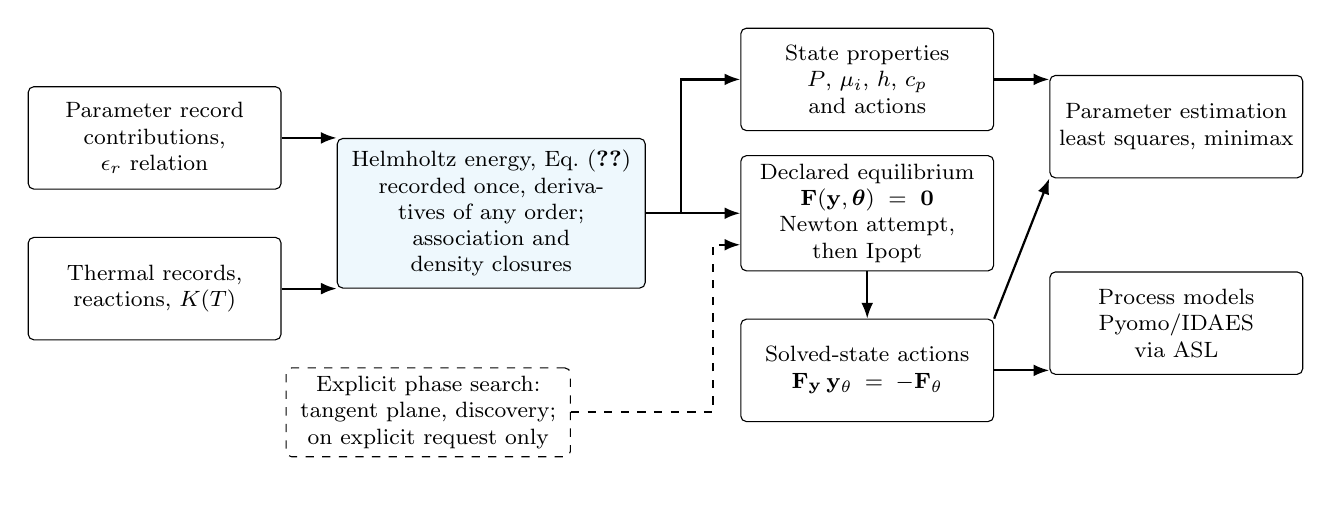
\begin{tikzpicture}[
  font=\footnotesize,
  box/.style={cse node, text width=30mm, minimum height=13mm},
  wide/.style={cse node, text width=37mm, minimum height=19mm, fill=cseSky!10},
  search/.style={cse node, text width=34mm, minimum height=11mm, dashed},
  flow/.style={cse arrow},
  node distance=6mm and 7mm]
  \node[box] (record) {Parameter record\\contributions, $\epsilon_r$ relation};
  \node[box, below=of record] (thermal) {Thermal records,\\reactions, $K(T)$};
  \node[wide, right=of $(record.east)!0.5!(thermal.east)$] (energy) {Helmholtz energy, Eq.~(\ref{eq:residual})\\recorded once, derivatives of any order;\\association and density closures};
  \node[box, right=12mm of energy, yshift=17mm] (state) {State properties\\$P$, $\mu_i$, $h$, $c_p$ and actions};
  \node[box, right=12mm of energy] (equil) {Declared equilibrium\\$\mathbf{F}(\mathbf{y},\boldsymbol\theta)=\mathbf{0}$\\Newton attempt, then Ipopt};
  \node[box, below=of equil] (actions) {Solved-state actions\\$\mathbf{F}_\mathbf{y}\,\mathbf{y}_\theta=-\mathbf{F}_\theta$};
  \node[search, below=10mm of energy, xshift=-8mm] (search) {Explicit phase search:\\tangent plane, discovery;\\on explicit request only};
  \node[box, right=of state, yshift=-6mm] (fit) {Parameter estimation\\least squares, minimax};
  \node[box, right=of actions, yshift=6mm] (process) {Process models\\Pyomo/IDAES via ASL};
  \draw[flow] (record.east) -- (energy.west |- record.east);
  \draw[flow] (thermal.east) -- (energy.west |- thermal.east);
  \draw[flow] (energy.east) -- ++(4.5mm,0) |- (state.west);
  \draw[flow] (energy.east) -- (equil.west);
  \draw[flow] (equil.south) -- (actions.north);
  \draw[flow] (state.east) -- (fit.west |- state.east);
  \draw[flow] (actions.east) -- (process.west |- actions.east);
  \draw[flow] (actions.north east) -- (fit.south west);
  \draw[flow, dashed] (search.east) -- (search.east -| {$(energy.east)+(8.5mm,0)$}) |- ([yshift=-4mm]equil.west);
  \path ([yshift=-3mm]current bounding box.south) node[inner sep=0] {};
\end{tikzpicture}

\caption{One native calculation serves every request.
A parameter record and declared thermal and reaction data define the Helmholtz energy of Eq.~\eqref{eq:residual} (Section~\ref{sec:model}), evaluated with its algorithmic derivatives on the selected support and thermal interval.
State properties, the rows of a declared equilibrium (Section~\ref{sec:equilibrium}) and the directional derivatives, called actions, of its solved state (Section~\ref{sec:derivatives}) are derivatives of that energy; parameter fits (Section~\ref{sec:estimation}) and process models consume them.
An explicit phase search uses the same driver but is never run inside a declared solve.
ASL, AMPL Solver Library.}
\label{fig:workflow}
\end{figure}



% P:introduction-06
Each comparison in this work answers one of four questions, and every figure panel is labelled with its class.
Numerical verification asks whether the code solves the stated equations; it compares results with independent codes, analytic identities and step refinement (Section~\ref{sec:verification}).
Published-model reproduction re-evaluates a published formulation and its parameters.
Comparison with calculated source values tests numerical translation; comparison with measured data or evaluated correlations instead assesses that published model while retaining its original fitting overlap and source limitations.
Calibration reports how well fitted parameters represent the data used to fit them, and prediction reports the error of fixed parameters on data outside the fit (Sections~\ref{sec:estimation} and~\ref{sec:physical}).
Inherited literature parameters may have been fitted to some of the data shown, so a prediction with such parameters is labelled with that overlap.
No comparison here is called physical validation, which would additionally require independent measurements with uncertainties, judged against a defined use.


% P:introduction-07
The examples span pure-fluid saturation, neutral and associating mixtures, electrolytes, solvent transfer and reacting phase splits.
The propane fit connects calibration to withheld-temperature prediction; mixed salts expose failed transfer from fitted binaries.
Sections~\ref{sec:model}--\ref{sec:estimation} introduce equations and algorithms, Section~\ref{sec:implementation} their use, and Sections~\ref{sec:physical} and~\ref{sec:verification} physical and numerical accuracy.
Cost, engineering use and limitations follow in Sections~\ref{sec:performance}--\ref{sec:conclusions}.


\begin{table}[pos=htbp]
\centering
\caption{Equilibrium and derivative capabilities of five PC-SAFT implementations, from their source code and documentation.
G, one general formulation shared with other specifications; S, a dedicated routine; P, partial or restricted scope; U, assembled by the user from lower-level outputs; X, excluded by the source or documentation; ?, not shown in the sources checked, which is unknown rather than absent.
The codes describe how a capability is provided, not its accuracy or cost.
An asterisk marks a class in which a comparison in Section~\ref{sec:verification} computes the same case with that code and this package.
Versions: FeOs~0.9.5 source, with 0.10.1 for the derivative, pressure--enthalpy and pressure--entropy flash and fitting classes; Clapeyron.jl development source following release~0.6.20, with the 0.6.29 documentation for implicit derivatives and the generalized flash; teqp~0.23.2; ThermoPack development source.
Supporting Information Section~\ref{sec:si-sources} gives the source of each cell.
\textsuperscript{a}Ions confined to the aqueous liquid or at trace amounts in the organic liquid.
\textsuperscript{b}Internal-energy--volume specifications and pressure--enthalpy or pressure--entropy specifications with charged species are not available.
\textsuperscript{c}Phase envelopes are verified for neutral vapor--liquid systems.
\textsuperscript{d}Derivative orders depend on the case and the input direction (Section~\ref{sec:derivatives}).
\textsuperscript{e}No physical comparison is reported in this work.}
\label{tab:software}
\small
\begin{tabularx}{\linewidth}{@{}Xccccc@{}}
\toprule
Problem class & This work & Clapeyron.jl & FeOs & teqp & ThermoPack \\
\midrule
Phase envelopes and critical points & G\textsuperscript{c} & S & S* & S* & S \\
Tangent-plane stability analysis & G & S & S* & ? & S \\
Neutral liquid--liquid and three-phase equilibrium & G & S* & S* & S & P \\
Electrolyte activity and osmotic coefficients & S & S* & U* & ? & X \\
Born solvation and composition-dependent permittivity & S & S* & S* & ? & X \\
Electrolyte vapor--liquid equilibrium with speciation & G\textsuperscript{e} & X & ? & ? & X \\
Electrolyte liquid--liquid equilibrium, ions in both liquids & G & S* & ? & ? & X \\
Simultaneous reaction and phase equilibrium & G & X & ? & ? & ? \\
Reactive electrolyte liquid--liquid equilibrium & G\textsuperscript{a} & X & ? & ? & X \\
Caloric properties and pressure--enthalpy flash & G\textsuperscript{b} & G & S* & G & S \\
Exact derivatives of equilibrium results & G\textsuperscript{d} & P* & P* & P & P \\
Electrolyte and reactive parameter estimation & S & P & ? & ? & ? \\
\bottomrule
\end{tabularx}
\end{table}

\section{Thermodynamic formulation and conventions}
\label{sec:model}
% P:model-01
A fluid phase $p$ is described by its species amounts $\mathbf{n}_p$ in mol, its total amount $N_p=\sum_i n_{p,i}$ and its volume $V_p$ in \si{\cubic\metre}.
Its mechanical Helmholtz energy is the ideal density and mixing term plus the residual term~\citep{Gross2001},
\begin{equation}
\frac{A_{p}}{RT}=\sum_i n_{p,i}\left[\ln\frac{n_{p,i}}{V_p\rho_0}-1\right]+N_p\,\ares\!\left(T,\frac{N_p}{V_p},\frac{\mathbf{n}_p}{N_p}\right),
\label{eq:phase-helmholtz}
\end{equation}
where $\rho_0=1$~\si{\mol\per\cubic\metre} is a fixed reference molar density and $\ares$ is the reduced residual molar Helmholtz energy at temperature $T$, molar density $\rho$ and mole fractions $\mathbf{x}$.
Ions are counted as separate species, so $\mathbf{x}$ of an electrolyte solution is a species, not a formula-unit, composition.
Thermodynamic properties and the chemical and mechanical equilibrium equations follow from derivatives of Eq.~\eqref{eq:phase-helmholtz} and the reference terms added in Section~\ref{sec:references}.
Conservation, electroneutrality and normalization supply the remaining equilibrium constraints (Section~\ref{sec:equilibrium}).
Supporting Information Table~\ref{tab:nomenclature} lists the symbols.

% P:model-02
The residual energy is a sum of contributions,
\begin{equation}
\ares=a^{\mathrm{hc}}+a^{\mathrm{disp}}+a^{\mathrm{assoc}}+a^{\mathrm{polar}}+a^{\mathrm{DH}}+a^{\mathrm{Born}},
\label{eq:residual}
\end{equation}
and a parameter record selects which contributions and which permittivity relation enter a calculation (Supporting Information Table~\ref{tab:contributions}).
A contribution that the record does not declare is identically zero, so Eq.~\eqref{eq:residual} is the selected formulation for a calculation, not a fixed inventory.
The hard-chain and dispersion terms are those of Gross and Sadowski, with a binary parameter $k_{ij}$ on the cross dispersion energy that may carry a declared temperature law~\citep{Gross2001,Held2014}.
The optional polar term is either the dipole--dipole contribution of Gross and Vrabec~\citep{Gross2006} or the quadrupole--quadrupole contribution of Gross~\citep{grossEquationofstateContributionPolar2005}; a record declares at most one of them, each is meaningful only with parameters fitted together with it, and no claim is made here for either one combined with ions.

% P:model-03
The association contribution follows Wertheim's theory in the form of Chapman et al.~\citep{Chapman1990},
\begin{equation}
a^{\mathrm{assoc}}=\sum_A x_{i(A)}\nu_A\left(\ln X_A-\frac{X_A}{2}+\frac12\right),\qquad
X_A\Bigl[1+\hat\rho\sum_B x_{i(B)}\nu_B X_B\Delta_{AB}\Bigr]-1=0,
\label{eq:mass-action}
\end{equation}
where $X_A$ is the fraction of sites of type $A$ not bonded and $\nu_A$ the number of such sites on species $i(A)$.
With $\rho$ in \si{\mol\per\cubic\metre}, the number density is $\hat\rho=10^{-30}N_A\rho$ in \AA$^{-3}$ and the association strength $\Delta_{AB}$ is in \AA$^3$, so $\hat\rho\Delta_{AB}$ is dimensionless.
Cross-association parameters follow the combining rule of Gross and Sadowski~\citep{Gross2002} or, when declared, that of Wolbach and Sandler~\citep{wolbachUsingMolecularOrbital1998}.
The site fractions are implicit functions of $(T,\rho,\mathbf{x})$ and of the parameters; Section~\ref{sec:derivatives} differentiates them through the mass-action system.

% P:model-04
The Debye--H\"uckel contribution is~\citep{Held2008,Bulow2019}
\begin{equation}
a^{\mathrm{DH}}=-\frac{\kappa e^2}{12\pi\epsilon_0\epsilon_r k_BT}\sum_{i}x_iz_i^2\chi(\kappa d_i^{\mathrm{DH}}),\qquad
\kappa^2=\frac{\rho N_A e^2\sum_i x_iz_i^2}{\epsilon_0\epsilon_r k_BT},\qquad
\chi(y)=\frac{3}{y^3}\Bigl[\ln(1+y)-y+\frac{y^2}{2}\Bigr],
\label{eq:dh}
\end{equation}
with charge numbers $z_i$, a separately declared closest-approach diameter $d_i^{\mathrm{DH}}$ and the bulk relative permittivity $\epsilon_r$.
The Born contribution is the corrected solvation-shell form of Figiel et al.~\citep{Figiel2025,Figiel2026Correction},
\begin{equation}
\begin{aligned}
a^{\mathrm{Born}}&=-\frac{e^2}{4\pi\epsilon_0k_BT}\sum_{i:z_i\ne0}x_iz_i^2\left[\frac{1-\epsilon_r^{-1}}{D_i}+c_{\mathrm{d}}\left(1-\epsilon_{r,\mathrm{ion}}^{-1}\right)\left(\frac{1}{d_i^{\mathrm{Born}}}-\frac{1}{D_i}\right)\right],\\
D_i&=d_i^{\mathrm{Born}}\left(1+c_{\mathrm{s}}\frac{f_{\mathrm{mix}}-1}{\lvert z_i\rvert}\right)\quad(z_i\ne0),
\end{aligned}
\label{eq:born}
\end{equation}
where $D_i$ is the outer shell diameter of ion $i$, and $f_{\mathrm{mix}}=\sum_jx_jf_j$ averages solvation factors over all neutral and ionic components, with $f_j=1$ for ions.
Here $\epsilon_{r,\mathrm{ion}}$ is the permittivity of the region between the ion and its shell, and $c_{\mathrm{s}}$ and $c_{\mathrm{d}}$ are fixed coefficients that recover the direct Born term when both are zero.
Both electrolyte contributions vanish identically on an ion-free support.
At zero ionic strength $a^{\mathrm{DH}}$ varies as the three-halves power of the ion amounts, which limits the derivatives available there (Section~\ref{sec:availability}).

% P:model-05
The relative permittivity enters Eqs.~\eqref{eq:dh} and~\eqref{eq:born} and must be declared consistently with the parameter record.
Four relations are available:
\begin{equation}
\epsilon_r=
\begin{cases}
\epsilon_{\mathrm{sf}}\big/\bigl(1+\sum_{i\in\mathcal I}\alpha_ix_i\bigr) & \text{ion suppression~\citep{Zuber2014,Figiel2025}},\\[2pt]
\epsilon_{\mathrm{sf}}\sum_{s\in\mathcal S}x_s+\sum_{i\in\mathcal I}x_i\epsilon_{r,i} & \text{component mixing~\citep{AscaniHeld2021,Bulow2019}},\\[2pt]
1+\rho\,x_{\mathrm{solv}}\,d_{V}\bigl(d_{T}/T-1\bigr) & \text{density--temperature~\citep{Yang2024}},\\[2pt]
1+3y\bigl\{1+y+\bigl[\tfrac{17}{16}I-1\bigr]y^2\bigr\} & \text{dipolar perturbation~\citep{Rueben2024}},
\end{cases}
\label{eq:permittivity}
\end{equation}
Here $\mathcal S$ is the set of neutral solvent species, $\mathcal I$ the set of ions, and $x_{\mathrm{solv}}=\sum_{s\in\mathcal S}x_s$ the total solvent mole fraction.
The salt-free solvent mixture has relative permittivity $\epsilon_{\mathrm{sf}}$; $\alpha_i$ is a dimensionless ion suppression coefficient and $\epsilon_{r,i}$ the relative permittivity assigned to ion $i$ in the component-mixing relation.
The coefficients $d_V$ and $d_T$ are averages of the solvent coefficients weighted by $x_s/x_{\mathrm{solv}}$, in \si{\cubic\metre\per\mol} and K, respectively, so $\rho x_{\mathrm{solv}}d_V$ and $d_T/T$ are dimensionless.
In the dipolar-perturbation relation, $y$ is a reduced dipole density and $I$ a dimensionless correlation integral.
The first two relations do not depend on density and describe condensed phases only; the last two tend to $\epsilon_r=1$ as $\rho\to0$.
Pressure, chemical potentials and caloric properties retain $\partial\epsilon_r/\partial\rho$, $\partial\epsilon_r/\partial T$ and $\partial\epsilon_r/\partial\mathbf{x}$ wherever the selected relation depends on them.
The density dependence also decides where a charged trial phase can be evaluated during a phase search (Section~\ref{sec:stability}).

\subsection{Reference states, reactions and units}
\label{sec:references}
% P:model-06
Nonreactive phase equilibrium at fixed temperature needs only Eq.~\eqref{eq:phase-helmholtz}.
Reaction equilibrium also requires the combinations of standard Gibbs energies constrained by the declared reaction targets (see below); a supplied reaction constant does not require a separate ideal-gas thermal record for every species.
Total caloric properties additionally require sufficient species thermal data to determine the reference contributions to enthalpy, entropy and heat capacity.
For a species with a supplied ideal-gas thermal record, the standard Gibbs energy on the density basis of Eq.~\eqref{eq:phase-helmholtz} is
\begin{equation}
\frac{g^{\circ}_{i,\rho}}{RT}=\frac{h^{\circ}_i(T)}{RT}-\frac{s^{\circ}_i(T,P_0)}{R}+\ln\frac{RT\rho_0}{P_0},\qquad
h^{\circ}_i(T)=\Delta_fh^{\circ}_i(T_{\mathrm{ref}})+\int_{T_{\mathrm{ref}}}^{T}C^{\circ}_{p,i}\,\mathrm{d}\tau,
\label{eq:reference}
\end{equation}
with the entropy integrated likewise from $s^{\circ}_i(T_{\mathrm{ref}},P_0)$.
The ideal-gas heat capacities $C^{\circ}_{p,i}$ are given as constant, polynomial, Shomate~\citep{shomateMethodEvaluatingCorrelating1954} in the convention of the NIST Chemistry WebBook~\citep{linstromNISTChemistryWebBook1997}, NASA seven- and nine-coefficient~\citep{gordonComputerProgramCalculation1994} or DIPPR~107~\citep{alySelfconsistentEquationsCalculating1981} correlations over declared temperature intervals.
Reaction targets and supplied thermal records can together determine reference contributions for species without their own records, provided no undetermined neutral combination remains.
Insufficient thermal data make the affected total caloric quantities unavailable; residual properties and reaction-equilibrium calculations remain available when their own input requirements are met.

% P:model-07
A reaction declares its stoichiometry and exactly one target: a constant affinity, a constant equilibrium constant, or the correlation
\begin{equation}
\ln K(T)=a+\frac{b}{T}+c\,\ln\frac{T}{T_{\mathrm{ref}}}+d\,T
\label{eq:lnK}
\end{equation}
on the density basis, for which the activity of species $i$ is $(\rho x_i/\rho_0)\exp(\mu_i^{\mathrm{res}}/RT)$.
A constant on an ideal-gas pressure basis, or one shifted by a standard state with constant reaction enthalpy and entropy, converts exactly into another correlation of the form of Eq.~\eqref{eq:lnK}.
A constant on a molality, infinite-dilution or pure-liquid basis is converted through the residual chemical potentials of the reference state, computed for one pure neutral solvent and a charge-neutral dilution path at each temperature and pressure of the solve; this conversion is called reference completion below.
Only charge-neutral combinations of ionic reference potentials are determined, so single-ion standard states remain a gauge choice.
A reaction constant constrains the standard Gibbs energies only along the reaction subspace; it does not by itself fix the absolute caloric properties of each species, which also require thermal anchors from Eq.~\eqref{eq:reference}.
Thermochemistry that is supplied together with a reaction target is checked against it in Gibbs energy, enthalpy and heat capacity, and an inconsistency is reported as an error rather than resolved in favor of either input.

% P:model-08
Parameters are explicit physical inputs in SI molar units: K, Pa, mol, \si{\cubic\metre} and \si{\joule\per\mol}, with molality in mol per kg of solvent.
Before a calculation the package admits only inputs in the mathematical domain of the selected equations: positive diameters, a declared site topology, records that the selected contributions consume, and a feed whose mole fractions satisfy $\lvert\sum_iz_ix_i\rvert\le10^{-12}$.
A record that no selected equation consumes is refused rather than ignored.
Admission says nothing about whether published parameters are valid at the requested state; that physical validity is the caller's declaration.

% P:model-10
Electrolyte coefficients use the declared molality standard state.
The neutral mean ionic combination obeys $\ln\gamma_\pm=(\nu_+\ln\gamma_++\nu_-\ln\gamma_-)/(\nu_++\nu_-)$, while solvent activity gives $\Phi=-\ln a_w/(M_w\sum_j\nu_jm_j)$ on the stated solvent-mass basis~\citep{HamerWu1972,Held2014}.
Here $M_w$ is solvent molar mass in kg/mol, $m_j$ formula-unit molality and $\nu_j$ its total ion stoichiometry.
Individual-ion conventions cancel only in the neutral combination; mixed-salt isopiestic coefficients retain their source-specific reference convention.

\subsection{Parameter records and their domains}
% P:model-09
A parameter set is part of the physical model.
Adding a polar or solvation contribution while keeping parameters fitted without it changes the model and does not isolate the physical effect of that contribution.
Similarly, changing the diameter in the Debye--H\"uckel or Born terms changes the formulation even when the printed dispersion parameters are identical.
Supporting Information Table~\ref{tab:records} groups the distributed records by their source and scientific role.
The scientific-input collection contains 38 source families, including observation and thermal records; 26 families contain canonical equation-of-state parameter documents.
Several records represent alternative or fitted declarations for the same system, so the number of records is not a count of independently validated fluids.
Source applicability can be incomplete; the temperature and pressure ranges actually compared are given with the results rather than inferred from successful numerical evaluation.

\section{Numerical evaluation of properties}
\label{sec:state}
\subsection{Association as an implicit calculation}
% P:state-01
A density-specified state takes temperature, molar density and normalized, charge-neutral species composition.
For an associating fluid, the native calculation first solves the mass-action system of Eq.~\eqref{eq:mass-action}.
Its unbonded-site fractions change with composition and molecular parameters, so their implicit response must enter both properties and fitting columns.

% P:state-02
The native association iteration starts at unit site fractions, with an analytic two-population estimate for sufficiently strong association.
It solves the analytic mass-action Jacobian by full-pivot LU decomposition and damps a Newton step to preserve $0<X_A\le1$.
When the Jacobian does not separate its pivots sufficiently, substitution supplies the update.
The mass-action residual, rather than the step length alone, decides convergence.
Table~\ref{tab:defaults} gives the default residual and work limits.
The implicit derivative calculation subsequently uses the unweighted defining Jacobian at the converged fractions; a singular or ill-conditioned system makes the affected derivative unavailable.
No composition floor is introduced to make that derivative appear regular.

\subsection{Pressure closure and mechanical branches}
% P:state-03
A pressure-specified state adds the scalar equation
\begin{equation}
P(T,\rho,\mathbf{x})=\rho RT\left[1+\rho\left(\frac{\partial\ares}{\partial\rho}\right)_{T,\mathbf{x}}\right]=P_{\mathrm{target}}.
\label{eq:pressure-closure}
\end{equation}
Pressure, its slope and, when required for root location, its curvature follow from the same energy~\citep{Gross2001}.
The density search operates in a bounded packing domain and first inspects the liquid side.
Resolved pressure brackets with positive slope can then identify a liquid root and a lower-density vapor root.
The requested branch selects the highest or lowest resolved stable root; an unspecified branch is ambiguous when several stable roots remain.
An anchor from a neighboring state instead defines a local window in which the root must be unique.
These choices matter at subcritical conditions because the same temperature, pressure and composition can have several density roots.

% P:state-04
Slope and curvature samples can shorten root location when they are consistent with a single mechanical loop.
Unresolved shape information returns the search to a finite logarithmic density scan, with spinodal bisection separating the stable pressure brackets.
When a sample contradicts that assumed shape, the interval is subdivided, and a root is accepted only if successive finer subdivisions show the same sign changes of $P-P_{\mathrm{target}}$.
Safeguarded Newton refinement remains inside each pressure bracket.
With $r=(P-P_{\mathrm{target}})/(\rho RT)$ and bracket width $\Delta\rho$, termination requires $|r|\le\tau_\rho$ and $\Delta\rho\,|\mathrm{d}r/\mathrm{d}\rho|\le\tau_\rho$, with a finite nonzero derivative; an exactly zero computed residual is also accepted.
An unresolved bracket at the refinement budget is reported as a failure.
A small reduced residual does not imply the same relative pressure error at low compressibility factor: the latter is the reduced residual divided by $P_{\mathrm{target}}/(\rho RT)$.
Association failures interrupt the relevant scan and preserve the failed density and cause, so a disconnected set of evaluable points cannot silently become a complete root search.

\begin{algorithm}[tbp]
\caption{Evaluation of a density- or pressure-specified state}
\label{alg:state}
\begin{algorithmic}[1]
\Require Selected parameters, $T$, $\mathbf{x}$, density or pressure, branch and requested quantities
\State Admit units, support, charge, topology and required thermal intervals.
\State Select the contributions and the derivative recording (Section~\ref{sec:derivatives}) for these species and this temperature interval.
\State At each trial density solve Eq.~\eqref{eq:mass-action}, preserving $0<X_A\le1$.
\State Stop the site solve only when its residual meets the requested criterion; otherwise report its cause.
\If{pressure is specified}
\State Locate liquid-side evidence and the requested pressure bracket using analytic slopes and curvature.
\State Use the logarithmic scan and spinodal subdivision when structured location is unresolved.
\State Refine stable crossings by safeguarded Newton; require both reduced-residual and bracket-width criteria, or an exactly zero computed residual.
\State Select the declared extreme root, or the unique root in the supplied anchor window.
\EndIf
\State Evaluate the requested ideal, residual or total quantities at this one state.
\State Differentiate association and pressure closure implicitly for requested actions.
\State Return values, achieved residuals and conditioning; keep failed quantities explicitly unavailable.
\end{algorithmic}
\end{algorithm}

% P:state-05
Algorithm~\ref{alg:state} returns a mechanically admitted state, distinguished from a globally stable phase.
Supporting Information Fig.~\ref{fig:si-F2-density-roots-1} shows the roots and spinodals found for propane and aqueous NaCl and the pressure closure of the benchmark requests.
Gibbs-energy comparisons across compositions belong to Section~\ref{sec:equilibrium}; finite density sampling cannot exclude every arbitrarily narrow additional loop.


\subsection{Property assembly and reuse}
% P:state-06
Property requests reuse the converged density, sites and required energy derivatives.
Selected quantities compute only their dependencies; total calorics consume thermal records, while residual quantities remain available without them.
A new support or thermal interval selects a corresponding recording of the same equations and refreshes the numerical state.

\section{Phase and reaction equilibrium}
\label{sec:equilibrium}
\subsection{Objective and constraints}
% P:equilibrium-01
At fixed temperature and pressure, fluid equilibrium minimizes the Gibbs energy of the declared phases,
\begin{equation}
\frac{G}{RT}=\sum_p\left[\frac{A_p}{RT}+\frac{PV_p}{RT}+\sum_i n_{p,i}\frac{g^{\circ}_{i,\rho}}{RT}\right],
\label{eq:gibbs}
\end{equation}
written in amount and volume coordinates so that no inner density solve is needed~\citep{Pereira2012}.
The minimization is subject to the conserved-moiety balances and to the electroneutrality of each phase that contains ions~\citep{Ascani2022,Tsanas2019,Tsanas2022},
\begin{equation}
\sum_pN_p\,\mathbf{B}\,\mathbf{x}_p=\mathbf{B}\,\mathbf{n}_{\mathrm{feed}},\qquad
\mathbf{z}\cdot\mathbf{x}_p=0,
\label{eq:balances}
\end{equation}
where the rows of $\mathbf{B}$ span the conserved moieties, the reactions span its null space, and every reaction conserves charge.
One electroneutrality row is omitted for a phase of nonzero amount, because the balances and the neutral feed imply it.
Without reactions $\mathbf{B}$ is the identity and Eq.~\eqref{eq:balances} reduces to species balances.
Balance rows replace reaction extents as coordinates, and the extents can be reconstructed from a solution.

% P:equilibrium-02
The first-order conditions of this minimum are, for every species $i$ on the support of phase $p$,
\begin{equation}
\mu_{p,i}-\boldsymbol{\lambda}\cdot\mathbf{B}_i-z_i\varphi_p=0,\qquad P_p(T,V_p,\mathbf{n}_p)=P,
\label{eq:stationarity}
\end{equation}
with balance multipliers $\boldsymbol\lambda$ and a charge multiplier $\varphi_p$ per phase, both in \si{\joule\per\mol}~\citep{Ascani2022,Pereira2012}.
Equal chemical potentials across phases and zero affinity, $\sum_i\nu_i\mu_{p,i}=0$, of every reaction $\boldsymbol\nu$ in the null space of $\mathbf{B}$ follow from Eq.~\eqref{eq:stationarity}; for ions, only electrochemical potentials are equal, and $\varphi_p$ corresponds to the phase potential $-F\psi_p$ up to a common gauge.
Each phase also satisfies its normalization $\sum_ix_{p,i}=1$.

% P:equilibrium-03
A specification is data on these rows, not a separate solver.
A phase amount may be free or pinned, for example at zero amount for an incipient phase, and temperature or pressure may be free.
With $k$ pinned amounts, $f$ free intensive variables and $e$ independent caloric rows, a square system requires $f=k+e$.
Temperature--pressure flashes, bubble and dew points, vapor fractions, pure-fluid saturation, critical-equation candidates, phase envelopes and pressure--enthalpy and pressure--entropy flashes are specifications of this one formulation (Table~\ref{tab:specifications}).
Reactions and ions are admitted in flashes and phase boundaries; critical-equation, envelope and pressure--enthalpy or pressure--entropy specifications are neutral, and no internal-energy--volume specification is provided.
Pinned amounts and caloric rows turn the minimization into a feasibility problem on the same intensive rows.
Pure stoichiometric solids enter the same objective through their standard Gibbs energy, with an amount complementarity at fixed temperature and pressure; no solid result is reported in this work.

\begin{table}[pos=htbp]
\centering\small
\caption{Specifications of the common equilibrium equations. $N_p$ denotes a phase amount; a zero-pinned phase is incipient. Reactions and ions are admitted in the ordinary flash and boundary declarations. Caloric, critical and envelope cases shown here are neutral.}
\label{tab:specifications}
\begin{tabularx}{\linewidth}{@{}p{0.25\linewidth}p{0.27\linewidth}X@{}}
\toprule
Specification & Fixed quantities & Free quantities and additional equations \\
\midrule
Temperature--pressure flash & $T,P$, feed, phase supports & Phase compositions, volumes and amounts \\
Bubble or dew pressure & $T$, feed, one $N_p=0$ & $P$ and incipient composition \\
Bubble or dew temperature & $P$, feed, one $N_p=0$ & $T$ and incipient composition \\
Specified phase fraction & $T$ or $P$, feed, one pinned $N_p$ & One intensive variable and all phase compositions \\
Pure saturation & $T$, pure feed, one $N_p=0$ & Common $P$ and distinct phase densities \\
Pressure--enthalpy or pressure--entropy flash & $P$, feed, extensive $H$ or $S$ & $T$, phase split and one caloric balance \\
Critical-equation candidate & Neutral composition and mode normalization & $T,P$, density and critical mode; zero quadratic and cubic forms \\
Phase envelope & Neutral feed, one $N_p=0$, one local path condition & $T,P$ and both compositions along continuation \\
\bottomrule
\end{tabularx}
\end{table}

\subsection{Coordinates, initialization and iteration}
\label{sec:driver}
% P:equilibrium-04a
Compilation reduces the conservation rows to independent balances, resolves the species allowed in each phase and checks the equation count.
For fluid phases, logarithmic compositions and packing fractions preserve their positivity and represent composition and volume.
Free phase amounts remain physical amount coordinates, scaled within the optimizer; free intensive variables and balance/charge multipliers complete the unknown vector.
Amounts and balance residuals scale with the feed basis, while chemical rows use $RT$ and pressure rows use the corresponding thermal density scale.
The logarithmic compositions have a lower bound that depends on each species' available inventory; it keeps the optimizer's coordinates finite and is not a minimum physical concentration.
The balance matrix supplies attainable amounts through linear programs, so a tiny available inventory need not be displaced by a uniform composition bound.

% P:equilibrium-04b
Initialization uses the declaration before solving its coupled equations.
For an eligible neutral two-phase temperature--pressure flash, feed-state fugacity estimates give $K_i=\phi_i^L/\phi_i^V$, and a bracketed Rachford--Rice root supplies
\begin{equation}
\sum_i\frac{z_i(K_i-1)}{1-\beta+\beta K_i}=0,\qquad
x_i=\frac{z_i}{1-\beta+\beta K_i},\quad y_i=K_ix_i.
\label{eq:rr-start}
\end{equation}
These estimates initialize amounts and compositions, after which the actual density roots are resolved.
Reacting starts first estimate liquid speciation by an ideal-solution element-potential iteration with frozen nonideal terms~\citep{gordonComputerProgramCalculation1994}.
A cold reacting incipient boundary can solve its finite phases at the pressure seed before forming the boundary start.
The seed is an estimate of the same equations, not an equilibrium conclusion or a measured phase composition.
A supplied start overrides the generated quantities it declares.

% P:equilibrium-04c
One driver solves the rows of Eqs.~\eqref{eq:balances} and~\eqref{eq:stationarity}, with first and second derivatives of the same Helmholtz energy.
For eligible ordinary calls it first applies an exact Newton iteration, factorized by full-pivot LU, with at most two step halvings.
This attempt covers neutral, nonreacting liquid/vapor boundaries with one zero-pinned amount and one free intensive variable, and full-positive-support two-phase temperature--pressure flashes.
Declared-start calls, continuation correctors, stability trials and caloric seed solves use Ipopt alone.
An admitted Newton result must satisfy the final residual, topology, density-branch and local checks.
Otherwise Ipopt~\citep{Wachter2006} solves the same rows from the original start using the exact Hessian of the Lagrangian.
When all phase amounts are free, Ipopt minimizes Eq.~\eqref{eq:gibbs} subject to Eq.~\eqref{eq:balances}, so Eq.~\eqref{eq:stationarity} are its first-order conditions; when an amount is pinned or a caloric or critical row is added, the objective is constant and every row is an equality constraint of a square feasibility problem.
Algorithm~\ref{alg:equilibrium} summarizes the sequence.

\begin{algorithm}[tbp]
\caption{A declared phase and reaction equilibrium}
\label{alg:equilibrium}
\begin{algorithmic}[1]
\Require Feed, phases and supports, reactions/references, pinned amounts, intensive and caloric data
\State Compile independent balances, references, coordinates, bounds and residual scales.
\State Construct a supplied or physical start; use speciation and phase estimates in their admitted domains.
\If{the ordinary neutral declaration admits the Newton attempt}
\State Solve the exact row Jacobian; damp within bounds and test the full final admission.
\State Return only if all requested criteria and branch checks are met.
\EndIf
\State Run Ipopt from the original start with exact constraint and Lagrangian derivatives.
\State Polish the returned positive point with contracting exact-Jacobian corrections.
\State Recompute balance, charge, normalization, pressure and stationarity defects.
\State Check distinct phases, density identity and local reduced curvature.
\If{a neutral, nonreacting liquid/vapor solve without a supplied start has failed}
\State Seek a lower-temperature source and correct back within the bounded shared work.
\State Reapply the target declaration's residual and branch checks.
\EndIf
\State Return the achieved quantities and unmet criteria, or the complete cause of no finite state.
\end{algorithmic}
\end{algorithm}

% P:equilibrium-04d
Ipopt stops on its own scaled optimality measure, which can leave the recomputed defining rows slightly above the requested tolerance; the polish removes that remainder.
The final polish accepts exact-Jacobian corrections only when raw defining-equation defects decrease and the point remains positive.
Trace balances are judged relative to their available inventory as well as on the feed scale.
Polish can extend beyond the ordinary step count while raw defects exceed the requested tolerance and work remains.
Table~\ref{tab:defaults} distinguishes caller-configurable accuracy criteria from budgets and policy constants.
A finite candidate that misses the requested accuracy remains explicitly identified.


\begin{table}[pos=htbp]
\centering\small
\caption{Default numerical criteria and budgets. The association, reduced-pressure and equilibrium-row residual tolerances are caller-configurable and dimensionless after the stated normalization. The other rows give work budgets and fixed policy values, including the polish and implicit-action criteria. Budgets bound work; initialization and separation constants do not certify accuracy.}
\label{tab:defaults}
\begin{tabularx}{\linewidth}{@{}p{0.34\linewidth}p{0.16\linewidth}X@{}}
\toprule
Quantity & Default & Meaning \\
\midrule
Association residual & $2\times10^{-13}$ & Infinity norm of the mass-action equations \\
Association iteration budget & 50 & Maximum site updates \\
Association relative pivot separation & $10^{-13}$ & Newton linear-system admission \\
Reduced pressure residual & $10^{-12}$ & $|P-P_{\mathrm{target}}|/(\rho RT)$ \\
Density refinement budget & 60 & Per root or spinodal refinement \\
Initial density intervals & 40 & Logarithmic scan, before adaptive subdivision \\
Equilibrium row residual & $10^{-10}$ & Recomputed scaled defining-row maximum \\
Ipopt inner factor & 0.1 & Multiplier of requested row tolerance for minimization; square feasibility uses the row tolerance \\
Ordinary polish steps & 3 & Contracting Newton corrections; extensions depend on remaining defects and work \\
Polish correction criterion & $10^{-12}$ & Scaled correction and local forward-error estimate \\
Equilibrium iteration budget & 200 & Default optimizer work limit \\
Phase coincidence distance & $10^{-6}$ & Composition or log-packing separation \\
Implicit-action backward error & $10^{-10}$ & Normwise residual of the Taylor linear solve \\
Implicit-action forward-error bound & $10^{-6}$ & Condition estimate combined with backward error \\
\bottomrule
\end{tabularx}
\end{table}

% P:equilibrium-04e
After designated ordinary neutral, nonreacting, nonassociating liquid/vapor failures without a supplied start, bounded recovery can seek a lower-temperature source and continue back.
Correctors retain phase identity and the target's residual and density-branch checks.
Recovery consumes its finite work allowance and supplies no phase-search conclusion.


% P:equilibrium-05
After either solution path, balance, charge, normalization, pressure and stationarity defects and phase distinctness are recomputed.
For free-amount minimization, stationarity in the logarithmic composition coordinates weights the dimensionless chemical rows by phase amount times mole fraction divided by feed amount; unscaled chemical-potential differences remain diagnostics.
Positive-definite reduced curvature on the constraint null space establishes a strict local minimum, while a coalesced declared phase set is reported as coincident.
Neither optimizer termination nor these local checks establish global equilibrium.


\subsection{Stability testing and phase discovery}
\label{sec:stability}
% P:equilibrium-06
Testing the stability of a result and discovering phases are explicit requests, separate from a declared solve, so a declared calculation never implies an unperformed search.
At the solved temperature and pressure, a trial composition $\mathbf{w}$ and molar volume $v$ have the tangent-plane distance~\citep{Michelsen1982,Pereira2012,Perdomo2025}
\begin{equation}
t(\mathbf{w},v)=\frac{a(\mathbf{w},v)}{RT}+\frac{Pv}{RT}+\mathbf{w}^{\mathsf T}\bigl(\mathbf{s}-\mathbf{B}^{\mathsf T}\boldsymbol{\lambda}\bigr),\qquad
\sum_iw_i=1,\quad\mathbf{z}\cdot\mathbf{w}=0,
\label{eq:tpd}
\end{equation}
where $a$ is the molar form of Eq.~\eqref{eq:phase-helmholtz}, $s_i=g^{\circ}_{i,\rho}/RT$ is frozen at the solved state, and $\boldsymbol\lambda$ is here the dimensionless balance multiplier.
Ionic and reacting trials are minimized through the same driver on unit-amount trial phases.
Neutral nonreacting searches first use Michelsen's substitution and second-order tangent-plane steps~\citep{Michelsen1982}, falling back to the shared driver when those iterations fail.
A negative distance counts as descent only with a positive donor phase that can supply the trial's species, and only when a finite inventory-conserving split lowers the computed Gibbs energy by more than its propagated numerical uncertainty.

% P:equilibrium-06b
Algorithm~\ref{alg:discovery} lists the search.
A trial phase is defined by its support, the species allowed in it, and a liquid or vapor label.
By default the supports are all fed and reacting species as a liquid, and their neutral subset as a liquid and as a vapor.
Each support receives a positive charge-neutral seed and, for each neutral species, a near-pure seed; compositions of phases removed earlier on the same support are added.
Each seed is minimized from every admitted density root, and failed roots remain in the returned list as unresolved trials.

% P:equilibrium-06c
Discovery tries descending phases in order, retaining an enlarged or reduced declaration only when it is admitted and lowers Gibbs energy beyond the estimated numerical uncertainty.
It refuses charged vapor additions even when the selected permittivity relation admits evaluating such a trial.
A completed finite search reports that no descent was found among the recorded trials, which is not a global stability certificate.

% P:equilibrium-07
Charged trial phases are admitted under every permittivity relation of Eq.~\eqref{eq:permittivity}, within its domain.
Under the density--temperature and dipolar-perturbation relations, which tend to the vacuum value at zero density, a charged trial counts at every density.
Under the density-independent relations the electrolyte terms describe condensed phases only, so a charged trial point counts only when it is a mechanically stable density root of its own composition on the liquid side of that composition's pressure loop.
A charged point on the vapor side, or one whose isotherm shows no loop, is unavailable with that cause and is never counted as descent.
This condition establishes condensed density only, not that the composition lies within the range over which the permittivity correlation was fitted.

\subsection{Inventories and zero amounts}
% P:equilibrium-09
For a declared feed, linear programs give the largest amount of each species, and its largest aggregate mole fraction, that the conserved balances allow with nonnegative amounts.
These bounds impose no energy condition and establish no equilibrium; they are nonsmooth, so no derivatives of them are supplied.
When a nonnegative conserved inventory of the feed is exactly zero, every species that carries it is absent from every phase, and the package removes those species before solving while keeping the original reactions and reference completion.
Zero carbon in an aqueous monoethanolamine (MEA) solvent, for example, removes the carbon-bearing species but keeps the protonated amine, hydronium and hydroxide ions, so zero carbon does not imply zero ionic strength.
On this zero-inventory face of the composition space the package also solves incipient liquid/vapor boundaries for exactly two opposite phases whose incipient support contains only uncharged species; these return a local boundary pressure and make no discovery or stability claim.
Derivatives that stay on the face differ from one-sided insertion of the absent species into it, which is treated in Section~\ref{sec:availability}.

\begin{algorithm}[H]
\caption{Explicit tangent-plane testing and phase discovery}
\label{alg:discovery}
\begin{algorithmic}[1]
\Require A solved state for testing, or a feed at fixed $T,P$ for discovery; admitted trial supports, density labels and finite work limits
\If{discovery is requested}
\State Solve union-liquid and, for a neutral union, union-vapor initial declarations; retain the admitted state with the lowest Gibbs energy.
\State Stop if no initial declaration is admitted.
\EndIf
\State Freeze actual reference terms at the solved $T,P$ and retain balance multipliers.
\State Enumerate distinct support/label pairs and positive charge-neutral seeds, including near-pure neutral seeds and compatible removed-phase compositions.
\For{each admitted seed and root}
\State Minimize the neutral tangent plane by substitution/second-order steps, or use the shared driver.
\State Reconstruct composition and density and apply the charged-domain rule.
\State Estimate tangent-plane uncertainty, require a positive full-support donor, and test a finite inventory-conserving split for a resolved Gibbs-energy decrease.
\EndFor
\State For testing, return the ordered trials, including unavailable and incomplete cases.
\State For discovery, stop explicitly if the trial search is incomplete or a negative tangent plane has unresolved finite descent; finish only if the completed search finds no resolved descent.
\State Try distinct descending trials in increasing donor slope, checking density identity and refusing charged vapor additions.
\State Solve each enlarged declaration; remove vanished or coincident phases when admitted, conserve inventory, retain their compositions as future seeds, and solve again.
\State Accept an addition only if the solved declaration meets its residual criterion and lowers Gibbs energy beyond the estimated numerical uncertainty.
\State Repeat testing at the accepted state, or stop explicitly when no lower-Gibbs-energy declaration is admitted or a work or rank limit is reached.
\end{algorithmic}
\end{algorithm}

\subsection{Critical candidates and phase envelopes}
% P:equilibrium-10
Criticality adds a normalized mode to a neutral one-phase declaration and imposes zero quadratic and cubic energy forms along that mode~\citep{bellImplementingEquationState2022}.
The augmented equations must have a full-rank Jacobian, and the computed curvature spectrum must place the candidate mode at the lowest unresolved-zero eigenvalue without a resolved negative mode below it.
The result is a critical-equation candidate; a separate stability calculation would be needed to assess other compositions.
For a phase envelope, a feed phase and an incipient phase have free temperature and pressure, closed by a selected local path condition.
A tangent from the defining Jacobian predicts the next state, and the common driver corrects it within density-anchor windows.
The largest dimensionless change in temperature, pressure or distribution coefficients selects a suitable path coordinate, while rejected steps are halved within the declared retry budget.
Figure~\ref{fig:search-envelope} shows one tangent-plane test and one traced envelope.

\begin{figure}[pos=H]
\centering
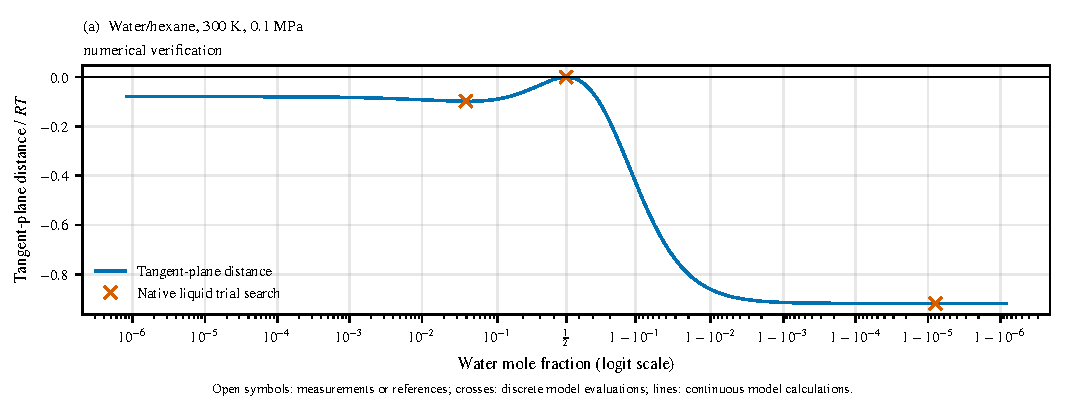
\includegraphics[width=0.96\linewidth]{F3-tpd-path}\par
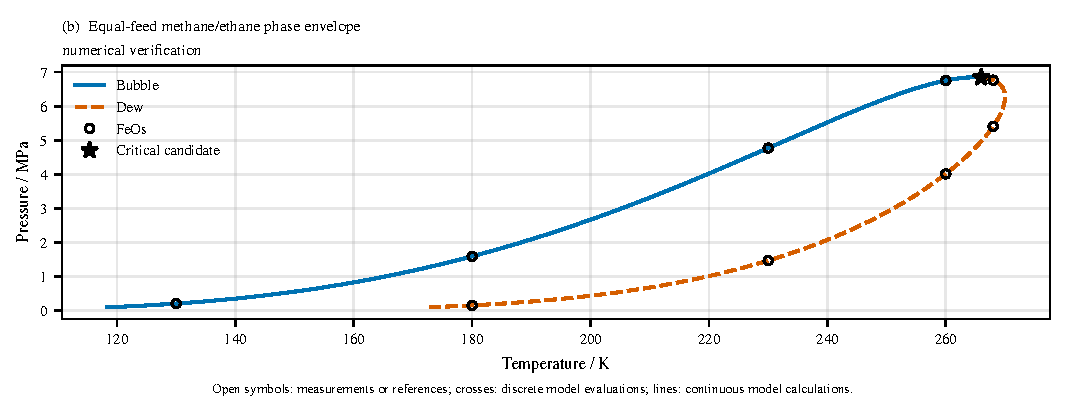
\includegraphics[page=1,width=0.96\linewidth]{F4-phase-envelope}
\caption{Phase search and envelope continuation (numerical verification).
Top: tangent-plane distance of a trial liquid against its water mole fraction for an equimolar water/hexane liquid at 300~K and 0.1~MPa, with crosses at the compositions returned by the liquid trial search of Algorithm~\ref{alg:discovery}.
The distance is zero at the feed and negative near both pure components, so the equimolar liquid is unstable as a single phase.
Bottom: bubble and dew curves of an equimolar methane/ethane mixture traced by continuation, with FeOs points and the critical-equation candidate; the remaining critical and bubble/dew comparisons are in the Supporting Information.}
\label{fig:search-envelope}
\end{figure}

\section{Exact derivatives and equilibrium calorics}
\label{sec:derivatives}
\subsection{Derivatives of the Helmholtz energy}
% P:derivatives-01
The package represents the residual Helmholtz energy of Eq.~\eqref{eq:residual} as an operation sequence of the CppAD algorithmic-differentiation library~\citep{bellCppADPackageAlgorithmic2025}, with temperature, volume, species amounts and the active parameters as independent variables.
Directional derivatives, called actions below, follow by forward propagation of Taylor coefficients through that sequence, with mixed derivatives obtained by polarization, which recovers a mixed derivative from derivatives along sums and differences of directions.
The interface supplies selected actions through third order on admitted smooth branches; the orders needed by each quantity and their availability are specified below.
The model reuses at most two recordings keyed by support, electrolyte predicates, thermal interval and output availability, and refreshes the numerical state on every call.
Property, equilibrium, fitting and process-model requests share this one evaluation, so a pressure, a chemical potential and an equilibrium Jacobian of the same state come from the same derivative chain.

% P:derivatives-02
The association site fractions of Eq.~\eqref{eq:mass-action} are solved by a native Newton iteration before the energy is evaluated.
For the mass-action residual $\mathbf{r}(\mathbf{X};\xi)=0$ on a branch where $\partial\mathbf{r}/\partial\mathbf{X}$ is nonsingular,
\begin{equation}
\frac{\partial\mathbf{r}}{\partial\mathbf{X}}\,\frac{\mathrm{d}\mathbf{X}}{\mathrm{d}\xi}=-\frac{\partial\mathbf{r}}{\partial\xi},
\label{eq:implicit}
\end{equation}
where $\xi$ is a temperature, density, composition or parameter direction; higher orders follow by differentiating Eq.~\eqref{eq:implicit} again.
A pressure-specified state is treated the same way: its density solves $P(T,\rho,\mathbf{x})=P$ on a branch with $\partial P/\partial\rho>0$, and the derivatives of every property at fixed pressure include the implicit response of the density.
The Born diameters held by declared hydration energies during parameter estimation (Section~\ref{sec:estimation}) are a third implicit system of this kind.

% P:derivatives-03
Exact here means that the derivatives are those of the stated discrete equations, obtained without finite differences.
They still carry floating-point rounding, the residual error of the converged association, density and hydration closures, and the conditioning of every linear solve; the comparisons of Section~\ref{sec:verification} measure these effects on the tested cases.
Finite differences are used only as references to verify exact derivatives.

\subsection{Derivatives of a solved state}
% P:derivatives-04
Let $\mathbf{F}(\mathbf{y},\boldsymbol\theta)=0$ collect the rows of Section~\ref{sec:equilibrium} that define a returned state: balances, electroneutrality, normalization, stationarity, pressure, pinned amounts and any caloric rows.
For fluid-phase declarations, the state coordinates $\mathbf{y}$ comprise phase amounts, logarithmic compositions and packing fractions, free intensive variables, and balance and charge multipliers.
The inputs $\boldsymbol\theta$ comprise temperature, pressure, feed amounts, active model parameters and reaction-law coefficients.
On a smooth branch with fixed supports and nonsingular $\mathbf{F}_\mathbf{y}$, the first and second directional actions along input directions $a$ and $b$ solve~\citep{pirnayOptimalSensitivityBased2012}
\begin{equation}
\mathbf{F}_\mathbf{y}\,\mathbf{y}_a=-\mathbf{F}_a,\qquad
\mathbf{F}_\mathbf{y}\,\mathbf{y}_{ab}=-\bigl(\mathbf{F}_{ab}+\mathbf{F}_{a\mathbf{y}}\mathbf{y}_b+\mathbf{F}_{\mathbf{y}b}\mathbf{y}_a+\mathbf{F}_{\mathbf{y}\mathbf{y}}[\mathbf{y}_a,\mathbf{y}_b]\bigr).
\label{eq:solved-actions}
\end{equation}
Third-order actions follow from the same recursion applied to the Taylor coefficients of $\mathbf{y}$ along a straight input path, with mixed directions recovered by polarization.
Each action uses linear solves with the shared central Jacobian factorization after row and column equilibration.
The inverse of the equilibrated Jacobian is formed only for the condition estimate; the linear-solve residual and that estimate are reported with the result.
The derivative of an observable adds its direct dependence on $\boldsymbol\theta$ to its dependence through $\mathbf{y}$.
At a given returned state, the actions depend on the shared defining rows and their derivatives, not on the iteration history used to obtain that state.

% P:derivatives-05
Each derivative order of a solved state needs one more order of the Helmholtz energy than the rows contain (Table~\ref{tab:orders}).
The stationarity rows contain first derivatives of the energy, so a first action needs second energy derivatives and a third action needs fourth.
Caloric observables add their own order: the enthalpy is a first derivative of the energy and the fixed-composition heat capacity a second.
The table states mathematical requirements; Section~\ref{sec:verification} states which observables and directions were verified.

\begin{table}[pos=htbp]
\centering
\caption{Order of Helmholtz-energy derivatives required by a value and its directional actions on a smooth branch. A table entry is a mathematical requirement, not evidence that every direction is verified.}
\label{tab:orders}
\small
\begin{tabular}{@{}lcccc@{}}
\toprule
Quantity & Value & First action & Second action & Third action \\
\midrule
$P$, $\mu_i$, residual $h$, $u$, $s$ & 1 & 2 & 3 & 4 \\
Fixed-composition $c_p$, $c_v$ & 2 & 3 & 4 & 5 \\
Solved state $\mathbf{y}$ & 1 & 2 & 3 & 4 \\
\bottomrule
\end{tabular}
\end{table}

\begin{algorithm}[tbp]
\caption{One request for exact actions of a solved equilibrium}
\label{alg:actions}
\begin{algorithmic}[1]
\Require Admitted central state, observables, input directions and requested orders
\State Recompute the classified defining-row residual and require it to be no larger than $\min(\tau_{\mathrm{row}},10^{-10})$.
\State Select support, thermal interval and reaction-reference derivatives for this request.
\State Assemble $\mathbf{F}_{\mathbf{y}}$, equilibrate its columns and rows by powers of two, and factor it once.
\State Refuse singular systems and directions that cross an unavailable support or reference domain.
\For{each required Taylor coefficient, in increasing order}
\State Propagate known lower coefficients through the common energy and reference equations.
\State Form the coefficient residual with the unknown highest state coefficient set to zero.
\State Solve with the central factorization for that highest coefficient.
\State Check backward error and the condition-based forward-error estimate.
\EndFor
\State Compose each observable with the state coefficients and its direct input dependence.
\State Recover mixed actions by polarization and report units, errors and unavailable causes.
\end{algorithmic}
\end{algorithm}

% P:derivatives-04b
Algorithm~\ref{alg:actions} differentiates the defining equations, independently of optimizer history.
Every highest unknown Taylor coefficient multiplies the same central Jacobian; known lower coefficients form the right-hand side.
One factorization therefore serves several directions and observables.
Action units follow the physical direction, and condition-based error estimates accompany the linear residual.


\subsection{Where derivatives are unavailable}
\label{sec:availability}
% P:derivatives-06
An action is returned only where Eq.~\eqref{eq:solved-actions} holds.
No action crosses a change of phase support, so no derivative describes the appearance or disappearance of a phase.
At a critical-equation candidate first- and second-order actions are available but third-order actions are unavailable, and pressure-specified quantities that divide by $\partial P/\partial\rho=0$ are unavailable.
With reactions referenced to a molality, infinite-dilution or pure-liquid basis, third-order actions admit only feed directions at fixed temperature and pressure, and second-order actions admit at most one parameter or reaction-law direction.
Because $a^{\mathrm{DH}}$ varies as the three-halves power of the ion amounts, second derivatives along an arbitrary ionic insertion direction are not finite at zero ionic strength.
Chemical potentials, fugacities and parameter columns of absent charged species are therefore reported as unavailable with that cause rather than as zero, while central values remain available.
Derivatives along the insertion of an association site that is absent from the support are not established.
Every unavailable action is reported with its cause and never as a number.

\subsection{Calorics of solved reacting equilibria}
% P:derivatives-07
On declared reacting branches with thermal records, the package returns caloric values of the solved equilibrium and their actions, including the completion of the reaction reference to fourth order in temperature and pressure and the apparent isobaric heat capacity
\begin{equation}
c_{P,\mathrm{eq}}=\frac{1}{N_{\mathrm{f}}}\left(\frac{\mathrm{d}H}{\mathrm{d}T}\right)_{P},
\label{eq:cpeq}
\end{equation}
where $H$ is the extensive enthalpy of all phases along the solved fixed-pressure path and $N_{\mathrm{f}}$ the feed amount.
$c_{P,\mathrm{eq}}$ contains the heat absorbed by the shift of the reactions and phase split with temperature, so it differs from the fixed-composition heat capacity of a phase.
It is a first-order action of $H$, its first temperature action is the second-order action, and higher actions of $c_{P,\mathrm{eq}}$ are not provided; it requires driven temperature and pressure.
It is not a reacting constant-volume heat capacity, and no internal-energy--volume specification is provided.

% P:derivatives-08
Reference completion contributes its own derivatives: a molality-based reaction law changes with the reference solvent state and its charge-neutral dilution limit as temperature or pressure changes.
The calculation determines neutral ionic combinations, not independent single-ion standards.
Finite-addition enthalpy columns likewise include both solved endpoints and the declared feed enthalpy.


% P:derivatives-09
At fixed pressure and feed, integrating $N_{\mathrm f}c_{P,\mathrm{eq}}$ should recover the independently solved enthalpy increment; integrating its temperature derivative should recover the heat-capacity increment.
Section~\ref{sec:derivative-verification} tests these numerical identities.
Measured calorimetry would be required to establish physical accuracy.

\section{Parameter estimation and measurement models}
\label{sec:estimation}
% P:estimation-01
A parameter fit compares observations $y_k$ with model predictions $\hat y_k(\boldsymbol\theta)$ through the scaled least-squares objective
\begin{equation}
\min_{\boldsymbol\theta}\ \tfrac12\sum_k w_k r_k(\boldsymbol\theta)^2,
\qquad r_k=\frac{\hat y_k(\boldsymbol\theta)-y_k}{s_k}\quad\text{or}\quad r_k=\ln(\hat y_k/y_k),
\label{eq:fit}
\end{equation}
where $s_k>0$ is a numerical scale in the observation's units for a difference residual, and $w_k\geq0$ is a dimensionless relative weight.
The log-ratio residual is dimensionless, has no separate scale and requires positive predicted and observed values.
The active coordinates $\boldsymbol\theta$ are affine maps of physical parameters: residual equation-of-state parameters such as $k_{ij}$, segment diameters or association energies, a scalar $\ln K$ on a reaction's declared basis, and the coefficients $a$, $b$, $c$ and $d$ of Eq.~\eqref{eq:lnK}; reactions are identified by name rather than by position.
The package minimizes Eq.~\eqref{eq:fit} within declared bounds with the Levenberg--Marquardt trust-region method of the Ceres solver~\citep{agarwalCeresSolver2023}.
Every state is solved once per trial point, and a state that fails to solve is a failed evaluation, never a zero residual.

% P:estimation-02
Prediction derivatives of solved observations, $\partial\hat y_k/\partial\theta_j$, are assembled from Eq.~\eqref{eq:solved-actions} with $\mathbf{y}_\theta=-\mathbf{F}_\mathbf{y}^{-1}\mathbf{F}_\theta$ evaluated as a linear solve.
The optimizer Jacobian multiplies each prediction derivative by $\sqrt{w_k}/s_k$ for a difference residual or $\sqrt{w_k}/\hat y_k$ for a log-ratio residual.
A reaction-law coordinate enters $\mathbf{F}_\theta$ only through the chemical rows.
Supporting Information Table~\ref{tab:observations} lists the observations whose columns are verified, with their active coordinates and verified domain.
Observations also include pressure-specified density, source-basis $\ln K$, phase compositions and fractions, bubble pressures, and the enthalpy of a finite addition between two solved endpoints, including a solvent with exactly zero conserved carbon.
Reaction-reference declarations stay fixed during a fit.
Qualified finite-addition enthalpy observations admit referenced endpoints with solved temperature, using the reference and caloric derivatives at each endpoint's temperature.
Other observations retain their stated domain limits, and an available state-derivative order implies no higher fitting order.
A local parameter covariance is reported from the scaled Jacobian when the fit ends in the interior of the bounds with full rank, and is withheld at an active bound or under rank deficiency.

\subsection{Measurement errors, correlated data and local uncertainty}
% P:estimation-06
The numerical scales and relative weights in Eq.~\eqref{eq:fit} do not by themselves specify measurement uncertainty.
The implemented measurement-error model is Gaussian and uses difference residuals with declared physical standard deviations and unit relative weights for the included observations.
When physical input uncertainty is declared, standardized corrections to measured temperature, pressure or admitted feed coordinates join the model parameters as unknowns.
The objective includes both the corrected-output errors and one penalty per shared input measurement.
A declared known covariance matrix can couple errors across observations and inputs.
Writing the standardized error vector as $\mathbf{e}$ and its covariance as $\mathbf{C}=\mathbf{L}\mathbf{L}^{\mathsf T}$ gives
\begin{equation}
\mathbf{L}\mathbf{z}=\mathbf{e},\qquad
\min\tfrac12\|\mathbf{z}\|_2^2,\qquad
\mathbf{L}\mathbf{J}_{z}=\mathbf{J}_{e}.
\label{eq:whitening}
\end{equation}
The matrix is factored once after symmetry and positive-definiteness checks; it is neither repaired nor replaced by a pseudoinverse.
The same triangular solve transforms every complete Jacobian column, preserving the connection between the objective and its derivatives.
A failed physical state remains a failed trial after whitening.

% P:estimation-07
Parameter covariance is conditional on the supplied error model and a regular local linearization.
Uncertain-input directions are eliminated from the complete standardized Jacobian.
Active bounds, deficient rank or unfinished fitting withhold covariance; known absolute uncertainties supply no estimated common-variance multiplier.
Local rank and covariance do not establish global identifiability or predictive accuracy.


\subsection{Electrolyte observations and guarded minimax fitting}
% P:estimation-03
For electrolytes, the observations include mean ionic activity and osmotic coefficients, ion solvation Gibbs energies and relative permittivities.
A Born diameter can be held by a declared hydration Gibbs energy: an inner root solve then makes the diameter a dependent coordinate, and the implicit first derivative of that root enters every Jacobian column.
The least-squares covariance is then conditional on the fixed hydration targets.

% P:estimation-04
Guarded minimax estimation instead minimizes the largest absolute decadic target error $t$,
\begin{equation}
\min_{\boldsymbol\theta,t}\ t\qquad\text{subject to}\quad \lvert e_k(\boldsymbol\theta)\rvert\le t\ \ (k\in\mathcal{T}),\qquad g_m(\boldsymbol\theta)\le g_m^{\mathrm{base}}\ \ (m\in\mathcal{G}),
\label{eq:minimax}
\end{equation}
where $e_k=\log_{10}(\hat y_k/y_k)$ is the target error in decades and the guard functions $g_m$ constrain error measures for selected properties outside the target set $\mathcal{T}$ relative to a declared baseline.
Ipopt solves this epigraph problem with exact first derivatives of the target and guard errors, obtained from the prediction columns, and limited-memory curvature, unlike the exact-curvature equilibrium solves of Section~\ref{sec:driver}.
Several native starts, sharing one iteration and time budget, test for distinct local solutions.
If recomputed feasibility and first-order optimality checks pass, the result is a local stationary estimate of Eq.~\eqref{eq:minimax}; optimizer termination alone does not establish stationarity.
The estimate supplies no covariance or guarantee of global optimality or parameter identification.

% P:estimation-05
Manufactured parameter recovery and refined-difference observation columns test numerical correctness in Section~\ref{sec:verification}.
The physical fits below instead report calibration and separated prediction.




\subsection{Worked propane and chloride fits}
% P:estimation-08
Propane provides a short fit that can be followed from observations to prediction.
Saturation pressures and saturated-liquid mass densities measured by Glos et al.~\citep{Glos2004}, Table~2, supply three training temperatures: 210, 270 and 330~K.
The active physical parameters are dispersion energy, segment number and segment diameter; the objective uses six natural-log ratios with unit weights.
Listing~\ref{lst:fit} shows the observation part of that declaration.
These numerical weights do not use the measured expanded uncertainties, so a low objective does not imply statistical agreement within those uncertainties.

\begin{lstlisting}[language={},caption={Observation excerpt of the propane fit declaration; the active physical coordinates are dispersion energy, segment count and diameter.},label={lst:fit}]
"targets": ["saturation_pressure", "saturated_liquid_mass_density"],
"residuals": {"saturation_pressure": "log_ratio",
              "saturated_liquid_mass_density": "log_ratio"},
"multiplier": 1.0
\end{lstlisting}

% P:estimation-09
Four starts reach the same local solution within the precision that matters for the property comparison.
The fitted parameters are $\epsilon/k=208.51125$~K, $m=1.9964556$ and $\sigma=3.6194291$~\AA.
The fit is interior and its local Jacobian has full rank, which permits a conditional covariance but supplies no validated prediction interval.
Figure~\ref{fig:fits} marks the three training temperatures, 19 withheld temperatures and two stress temperatures, 110 and 340~K, at the ends of the measured range.
The withheld temperatures include 150~K, which the source baseline lists as a training state but this fit does not use.
On the withheld temperatures the fitted parameters give pressure and liquid-density average absolute relative deviations (AARDs) of 1.00\,\% and 0.180\,\%, against 1.07\,\% and 0.228\,\% for the published parameters; the two stress states give 22.0\,\% and 0.382\,\% after fitting.
The refit therefore mainly improves the liquid density; the withheld pressure deviation changes little.
These populations include extrapolation below the training range; no pooled accuracy is assigned to an arbitrary new temperature.

\begin{figure}[pos=p]
\centering
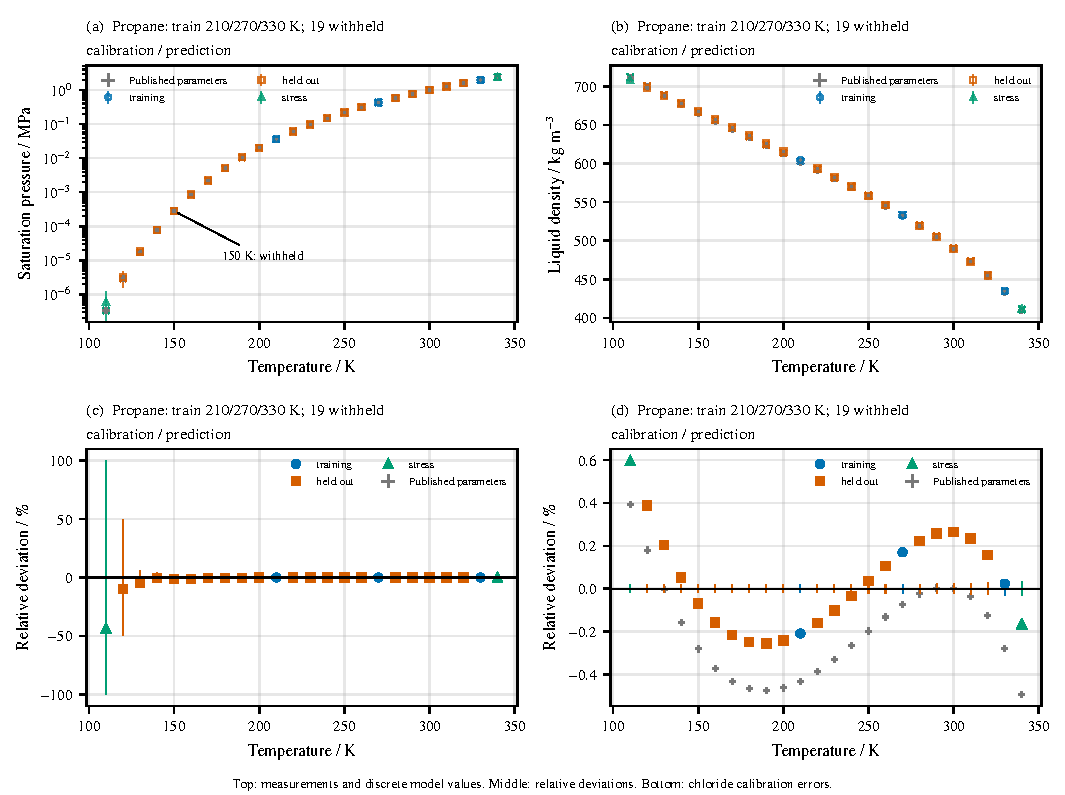
\includegraphics[width=0.91\linewidth,height=0.45\textheight,keepaspectratio]{F15-propane-fit}\par
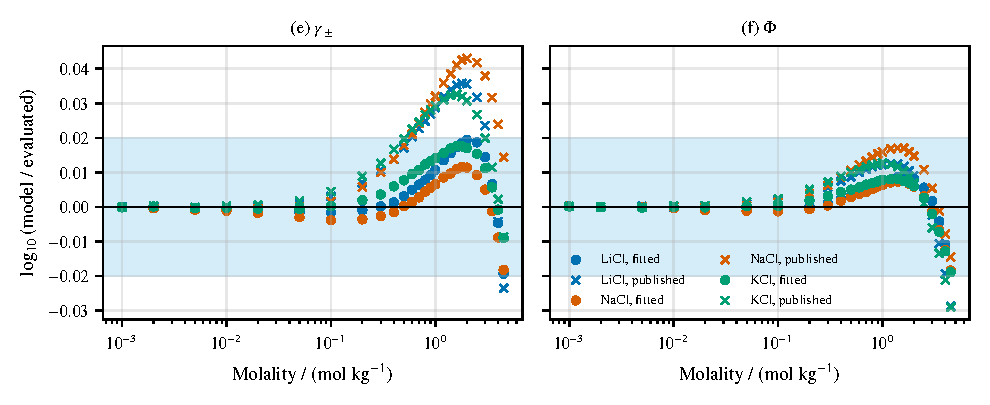
\includegraphics[width=0.91\linewidth,height=0.25\textheight,keepaspectratio]{chloride-calibration}
\caption{Calibration and transfer are separate parts of parameter estimation.
Top four panels: propane saturation pressure and liquid density against the measurements of Glos et al.\ after the three-temperature fit, with training, withheld and stress temperatures marked; in the deviation panels, bars are the expanded measurement uncertainties and grey crosses are the published parameters~\citep{Glos2004,Gross2001}.
Bottom: decadic errors $\log_{10}(\text{model}/\text{evaluated})$ of the mean ionic activity and osmotic coefficients of LiCl, NaCl and KCl at 298.15~K for the guarded minimax fit and the published parameters, with the $\pm0.02$ target band shaded~\citep{HamerWu1972,Figiel2025}.
The chloride data were fitted, so the bottom panels show calibration only.}
\label{fig:fits}
\end{figure}

% P:estimation-10
The electrolyte example uses a different objective for a different purpose.
Guarded minimax fits LiCl, NaCl and KCl activity and osmotic coefficients to the evaluated Hamer--Wu data~\citep{HamerWu1972}, Tables~9, 16 and~28, at 298.15~K and 100~kPa.
The 156 target quantities span 26 molalities per salt from 0.001 to 4.5~mol/kg.
Hydration targets hold Born diameters, and guards constrain bromide coefficients, transfer energies and aqueous permittivity relative to the published Figiel parameters~\citep{Figiel2025}.
The largest fitted target error is below 0.019371 decade, inside the declared 0.02-decade band; the published parameters exceed that band on 41 target rows.
A least-squares optimum also meets the target band but violates eight guard groups.
Thus the choice of estimator encodes which property deterioration is allowed, not merely which optimizer gives the smallest target sum.
Neither fit identifies unique electrolyte parameters or establishes independent mixture accuracy.

\section{Implementation, practical use and testing practice}
\label{sec:implementation}
% P:implementation-01
Every iterative calculation runs natively in C++: association and density closure, equilibrium solves, phase searches, continuation and parameter fitting.
The Python interface declares inputs and reads results; it supplies no callback to a native iteration and performs no thermodynamic arithmetic.
A caller constructs a model once from a parameter record.
Construction validates the species, site topology and model selection, admits the records of Section~\ref{sec:references}, and prepares state-independent quantities; support and thermal intervals select reusable recordings of the shared energy equations.
A state request then gives temperature, composition and exactly one of density or pressure; a pressure request resolves the declared density branch once and reuses that state for every property and derivative asked of it.
An equilibrium request is a declaration of phases, supports, pinned amounts, free intensive variables, feed and reactions, compiled once into the rows of Section~\ref{sec:equilibrium}.
Figure~\ref{fig:workflow} shows how these requests share one calculation.

% P:implementation-02
Listing~\ref{lst:example} declares a methane/ethane mixture with the parameters of Gross and Sadowski~\citep{Gross2001}, solves a bubble point at 200~K and requests the exact first-order response of the bubble pressure to temperature.
The same request with feed or parameter directions, or with phase compositions as observables, returns the other columns of $\mathbf{y}_\theta$ for that state.

\noindent\begin{minipage}{\linewidth}
\begin{lstlisting}[caption={A bubble point and its exact temperature derivative.},label={lst:example}]
import epcsaft
from epcsaft import equilibrium as eq

record = "data/packets/gross-2001-methane-ethane/3/parameters/parameters.json"
mix = epcsaft.Mixture(epcsaft.Parameters.from_json(record, components=["methane", "ethane"]))
feed = eq.MoleFractions({"methane": 0.3, "ethane": 0.7})
problem = eq.bubble_point(liquid=eq.Phase("L", kind="liquid"), T=200.0, feed=feed)
bubble = eq.solve_equilibrium(mix, problem)          # pressure is free
print(bubble.pressure, bubble.phase_mole_fractions(1))   # Pa; incipient vapor

dT = eq.SolvedStateActionDirection(1.0, 0.0, [0.0, 0.0], [ ])  # unit temperature direction
P = eq.SolvedStateObservable(eq.SolvedStateObservableKind.Pressure)
batch = eq.solved_state_actions(eq.compile_problem(mix, problem), bubble,
                                eq.SolvedStateActionRequest([P], [dT]))
print(batch.results[0].action, batch.results[0].status)       # Pa/K
\end{lstlisting}
\end{minipage}

% P:implementation-03
Equation-oriented process models reach the same calculation through a compiled library that implements external functions of the AMPL Solver Library.
A model written in Pyomo~\citep{hartPyomoModelingSolving2011}, for example within the IDAES process modeling framework~\citep{leeIDAESProcessModeling2021}, calls these functions and receives values with exact first and second derivatives.
The functions verified here return the pressure of a neutral fluid with its gradient and Hessian, and the phase compositions and amounts of a declared fixed-temperature, fixed-pressure, nonreactive two-liquid electrolyte split with their first and second feed derivatives.
It solves each call with the same native driver and adds no phase search.

% P:implementation-04
The native code depends on CppAD~20250000.3~\citep{bellCppADPackageAlgorithmic2025} for algorithmic differentiation, Ipopt~3.11.9~\citep{Wachter2006} with the MUMPS sparse linear solver~\citep{amestoyFullyAsynchronousMultifrontal2001,amestoyPerformanceScalabilityBlock2019} for equilibrium and minimax problems, Ceres~2.2~\citep{agarwalCeresSolver2023} for least squares, Eigen~3.4~\citep{guennebaudEigenV32010} for dense linear algebra, and HiGHS~1.15.1~\citep{huangfuParallelizingDualRevised2018} for the conserved-inventory linear programs.
The Python interface is built with nanobind~2.12.0~\citep{jakobNanobindTinyEfficient2022}.


\subsection{Testing and verification practice}
% P:implementation-05
Checks follow the dependency of a request: contribution equations, implicit closures, equilibrium balances and phase identity, derivative actions, then observation composition and process transport.
This helps distinguish an accurate property evaluation from a wrong root or an inaccurate physical model.


% P:implementation-06
The comparisons include 704 branch-specific density requests, 36 pressure-specified caloric actions and 3\,167 electrolyte observation columns, with reference values, identities, independent codes and refinement chosen by quantity.
Table~\ref{tab:verification} states representative numerical bounds.
Counts describe checked requests or scalar comparisons, not independent experiments.


% P:implementation-07
Practical use starts with a parameter record and specification, followed by inspection of achieved residuals, unavailable causes and source domains.
For external functions, the process model owns its balances, constraints and optimization, while the package owns the supplied properties or declared equilibrium and their derivatives.
An external flash may therefore assemble its own equilibrium equations from the package's properties, as illustrated in Section~\ref{sec:applications}.

\section{Model against measured data}
\label{sec:physical}
\subsection{Comparison basis, coverage and error measures}
% P:physical-01
The central physical question is how well a declared model, with a stated parameter choice, represents the measured quantities that an engineering calculation consumes.
The comparisons below cover several fluid classes and properties rather than seeking one accuracy number for the package.
A source may supply measured observations, an evaluated reference equation, or values from its own fitted model.
Those references remain separate throughout the galleries and Table~\ref{tab:physical-summary}.
Figure~\ref{fig:coverage} maps the comparisons; a blank cell means that the displayed evidence supplies no comparison, not that the corresponding calculation is mathematically impossible.
The main text shows representative systems for each fluid class; the Supporting Information table and galleries contain all 356 comparison populations, including parameter alternatives, fitted and withheld data, failed comparisons and unavailable states.

\begin{figure}[pos=H]
\centering
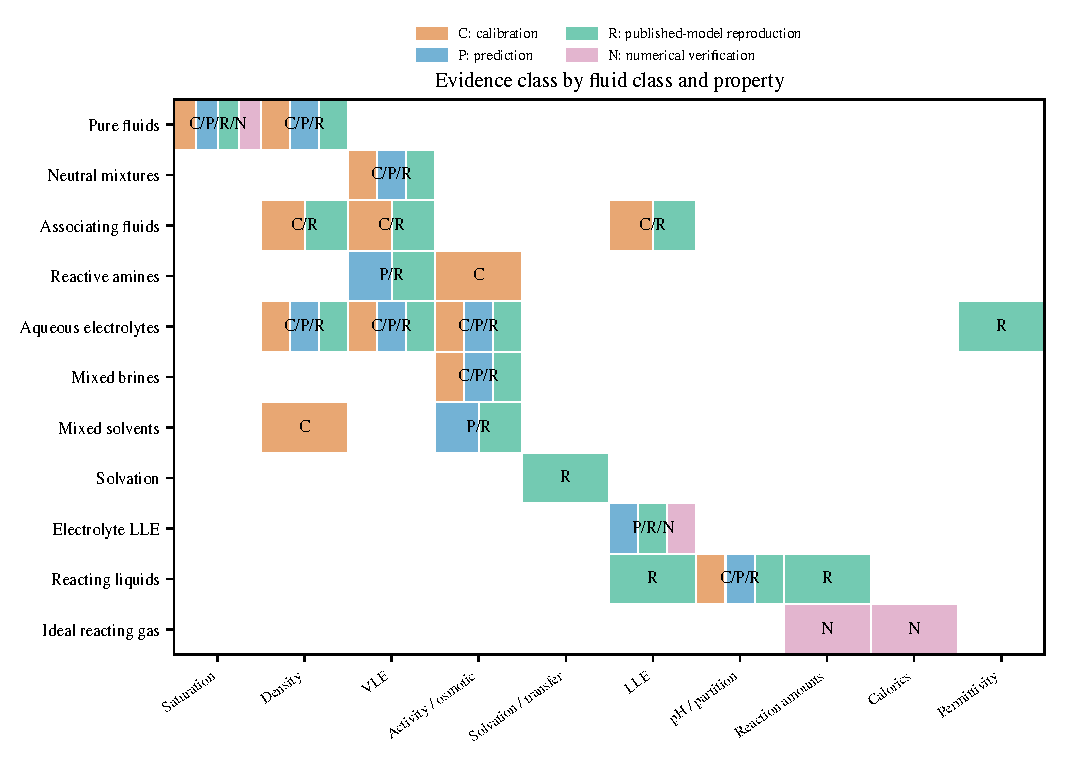
\includegraphics[width=0.94\linewidth]{F7-coverage}
\caption{The comparisons cover different physical quantities and evidence classes.
Calibration, prediction, published-model reproduction and numerical verification are distinguished, including split cells where more than one class applies.
Blank cells have no comparison in this work, and the map gives neither an accuracy ranking nor a count of independent datasets.
The per-population conditions, parameters and errors are given in Table~\ref{tab:physical-summary} and the complete Supporting Information table.}
\label{fig:coverage}
\end{figure}

% P:physical-02
For positive properties, the average absolute relative deviation is
\begin{equation}
\mathrm{AARD}=\frac{100}{n}\sum_{k=1}^{n}\left|\frac{y_k^{\mathrm{model}}}{y_k^{\mathrm{ref}}}-1\right|.
\label{eq:aard}
\end{equation}
Absolute mole-fraction and pH errors instead use the mean absolute error, and dimensional residuals or dimensionless coefficients can be summarized by a root-mean-square difference.
The table names the metric and unit because a pressure percentage, a pH-unit difference and an osmotic-coefficient residual cannot share a common accuracy scale.
Unavailable predictions remain identified, with statistics taken over the available comparisons rather than assigning a fictitious value to a failed solve.
Counts of repeated parameter variants or thermodynamically linked coordinates do not increase the number of independent measurements.

% P:physical-02b
Table~\ref{tab:physical-summary} gives the result by fluid class, and the subsections below explain each entry.
With published parameters, pure-fluid saturation pressures and liquid densities deviate from measurements or reference correlations by 0.281--2.70\,\% on average, and the zero-interaction methane/ethane prediction places both phase compositions within 0.008 mole fraction on average.
For aqueous 1:1 salts at 298.15~K the osmotic and mean ionic activity coefficients deviate by 1.72\,\% and 4.36\,\% from evaluated data that overlap the original parameter fit, and salted water/ethanol/isobutanol tie lines computed with the source parameters differ from the measurements by a mean 0.0111 mole fraction.
Accuracy is lost where parameters are carried beyond the data they were fitted to: unchanged published parameters fail every comparison range for NaCl--MgCl$_2$ and NaCl--CaCl$_2$ brines, NaCl activity coefficients deviate more in ethanol-rich than in water-rich solvents, the acetic acid partition coefficient deviates by 47.8\,\% although the aqueous pH is predicted within 0.146 unit, and MDEA parameters fitted to osmotic coefficients give total pressures with 96.2\,\% and 89.6\,\% AARD.
Refitting recovers a description within the fitted domain: a joint chloride fit predicts two withheld mixed-brine sources with RMS residuals of 0.00825 in osmotic coefficient and 0.00121 in water activity.
Section~\ref{sec:verification} shows that independent codes with matched models reproduce the package's state values to better than $10^{-8}$, so deviations of the size reported here belong to the model and its parameters, not to the numerical solution.



\begin{table}[pos=htbp]
\centering\footnotesize
\caption{Representative populations from the full comparison table. $N$ counts the displayed source rows; the methane/ethane comparison includes one unavailable state, and each aqueous 1:1-salt population includes 23 unavailable LiI rows. Their error means use 16 and 184 available comparisons, respectively. PRED denotes fixed-parameter prediction, CAL calibration and REPRO published-model reproduction. Original fitting overlap can remain unknown for inherited parameters. Pressure ranges are reference values; ``sat.'' denotes saturation with no separately reported density-row pressure.}
\label{tab:physical-summary}
\begin{tabularx}{\linewidth}{@{}p{0.19\linewidth}p{0.13\linewidth}p{0.13\linewidth}rX@{}}
\toprule
System / property & $T$/K & $P$/MPa & $N$ & Parameter role; error metric and value \\
\midrule
Propane / $P_{\rm sat}$ & 110--340 & $6\times10^{-7}$--2.43 & 24 & Gross--Sadowski; PRED, AARD 2.70\,\% \\
Propane / $\rho_L$ & 90--340 & sat. & 27 & Same; PRED, AARD 0.305\,\% \\
Propane / $\rho_V$ & 230--340 & sat. & 12 & Same; PRED, AARD 1.52\,\% \\
\ce{CO2} / $P_{\rm sat}$ & 220--300 & 0.599--6.71 & 17 & Gross quadrupolar; REPRO against reference equation, AARD 0.421\,\% \\
Benzene / $P_{\rm sat}$ & 290--540 & 0.00856--3.71 & 26 & Gross quadrupolar; REPRO against correlation, AARD 0.281\,\% \\
Methane/ethane / $x_{\ce{CH4}}$ & 203.22--243.61 & 2.124--6.885 & 17 & $k_{ij}=0$; PRED, MAE 0.00789 \\
Methane/ethane / $y_{\ce{CH4}}$ & 203.22--243.61 & 2.124--6.885 & 17 & $k_{ij}=0$; PRED, MAE 0.00412 \\
\ce{CO2}/THF / $x_{\ce{CO2}}$ & 313.2--353.2 & 0.47--10.29 & 34 & Schick inherited fit; REPRO/physical comparison, AARD 6.94\,\% \\
Aqueous 1:1 salts / $\gamma_\pm$ & 298.15 & 0.101 & 207 & Figiel inherited fit overlap; CAL, AARD 4.36\,\% \\
Same / $\Phi$ & 298.15 & 0.101 & 207 & Same; CAL, AARD 1.72\,\% \\
Joint chloride fit / $\Phi$ & 298.15 & 0.1 & 443 & Fitted source families; CAL, RMS 0.00748 \\
NaCl/\ce{CaCl2} / $\Phi$ & 298.15 & 0.1 & 53 & Joint fit, withheld source; PRED, RMS 0.00825 \\
NaCl/\ce{MgCl2} / $a_w$ & 298.15 & 0.1 & 19 & Joint fit, withheld source; PRED, RMS 0.00121 \\
NaCl/ethanol--water / $\gamma_\pm$ & 298.15 & unreported & 123 & Fixed Figiel parameters; PRED, AARD 6.35\,\% \\
Acetic acid/water/toluene / pH & 298.15 & 0.1 & 19 & Ascani, no pH fit; PRED, MAE 0.146 pH unit \\
Same / acid partition & 298.15 & 0.1 & 19 & Acid--organic calibration family; CAL, AARD 47.8\,\% \\
MDEA/\ce{CO2} / $P$ & 303 & 0.92--2.45 & 3 & Osmotic-fit S0/S1; PRED, AARD 96.2/89.6\,\% \\
\bottomrule
\end{tabularx}
\end{table}

\subsection{Pure nonpolar, dipolar and quadrupolar fluids}
% P:physical-03
Propane saturation with the Gross--Sadowski parameters~\citep{Gross2001}, Table~2, is compared with the later measurements of Glos et al.~\citep{Glos2004} in Supporting Information Fig.~\ref{fig:si-F8-pure-fluids-1} and, beside the refit, in Fig.~\ref{fig:fits}.
Pressure, liquid density and vapor density have different temperature populations and therefore separate statistics.
The pressure AARD of 2.70\,\% is larger than the liquid-density AARD of 0.305\,\%, with low-temperature pressures contributing strongly to the relative-pressure statistic.
The liquid-density observations are not all accompanied by a separately tabulated pressure in the selected population, so the table describes them as saturated states rather than inventing a pressure range.
The source expanded uncertainties are retained in the figure; they are not replaced by the numerical pressure-closure criterion.
All twelve vapor-density predictions lie outside their supplied uncertainty intervals; the low-temperature pressure discrepancy at 110~K lies inside its much larger interval.
The two coldest states, 110 and 120~K, where the measured pressures are 0.6 and 3.2~Pa, contribute 2.27 of the 2.70 percentage points; on the 19 temperatures withheld from the fit of Section~\ref{sec:estimation}, the published parameters give 1.07\,\% and 0.228\,\%.

% P:physical-04
The larger nonpolar catalogue contains one saturation calculation for each of 78 compounds from Gross and Sadowski~\citep{Gross2001}.
It establishes calculation breadth only: those catalogue states have no measured references from which to compute a 78-compound validation statistic.
Sparse source comparisons for methane, propylene, toluene and diethyl ether add liquid-density observations and paper-model samples in the Supporting Information.
At the coldest diethyl ether state the density misses the pressure-closure criterion, and at the coldest propylene state no density is returned; both states are marked and neither supports an accuracy statement.
The deviations that Gross and Sadowski report over their whole fitting datasets cannot be recomputed, because those observations are not available.

% P:physical-05
Dipolar acetone, dimethyl ether, diethyl ether and dimethyl sulfoxide test the optional Gross--Vrabec contribution~\citep{Gross2006} (Fig.~\ref{fig:pure-data}).
Published polar parameters, polar refits and nonpolar refits are distinct models in the full gallery.
Alternating training and withheld temperatures apply to the local refits.
The references for acetone, dimethyl ether and diethyl ether are the reference equations of state of Lemmon and Span~\citep{lemmonShortFundamentalEquations2006}, Wu et al.~\citep{wuEquationStateThermodynamic2011} and Thol et al.~\citep{tholNewFunctionalForm2014}, evaluated with CoolProp~8.0.0~\citep{bellPurePseudopureFluid2014}; they may share experimental data with the original published fit.
For acetone, the polar refit gives withheld pressure and liquid-density AARDs of 1.30\,\% and 0.669\,\%, compared with 0.936\,\% and 2.43\,\% for the nonpolar refit.
The example shows a property tradeoff: a smaller pressure error alone does not rank the overall formulation.
Because each formulation has its own fitted parameters, the difference cannot be attributed solely to switching on a dipole term at fixed parameters.
The DMSO measurements~\citep{Fulem2011,DePablo2018,Zhang2013,Paknejad2019} provide a separate source role and are not pooled with the evaluated reference equations as equivalent independent experiments.

\begin{figure}[pos=H]
\centering
\includegraphics[page=4,width=0.94\linewidth]{F8-pure-fluids}
\caption{Saturation pressure and liquid density of acetone, diethyl ether, dimethyl ether and dimethyl sulfoxide with the published polar parameters of Gross and Vrabec and with local polar and nonpolar refits~\citep{Gross2006}.
The refits use alternating training and withheld temperatures; references are reference equations of state for the first three fluids and measurements for dimethyl sulfoxide~\citep{lemmonShortFundamentalEquations2006,wuEquationStateThermodynamic2011,tholNewFunctionalForm2014,Fulem2011,DePablo2018,Zhang2013,Paknejad2019}.
Propane against the Glos measurements is in Fig.~\ref{fig:fits} and, with vapor densities, in the Supporting Information.}
\label{fig:pure-data}
\end{figure}

\begin{figure}[pos=H]
\centering
\includegraphics[page=5,width=0.94\linewidth]{F8-pure-fluids}
\par\small Figure~\ref{fig:pure-data} (continued).
\end{figure}

% P:physical-06
The quadrupolar parameters of Gross~\citep{grossEquationofstateContributionPolar2005}, Table~A1, are evaluated for carbon dioxide and benzene.
Their saturation-pressure AARDs are 0.421\,\% and 0.281\,\%, respectively, against the reference equation of Span and Wagner for carbon dioxide~\citep{spanNewEquationState1996}, evaluated with Clapeyron.jl, and a benzene vapor-pressure correlation.
These comparisons are identified as published-model reproduction against evaluated references.
They are useful tests of the selected model's pressure behavior over the displayed ranges, but they do not recover the original experimental fitting membership.
The benzene reference uses a DIPPR-101-form correlation whose coefficient attribution to the original compilation is unverified.
The nonpolar curves use their own parameters and therefore do not measure an isolated quadrupole correction.



\subsection{Neutral and polar mixture phase equilibria}
% P:physical-07
The methane/ethane comparison uses May et al.~\citep{May2015}, Table~5, with the Gross--Sadowski pure parameters and $k_{ij}=0$.
The measured liquid and vapor compositions define the physical references, while midpoint feeds are calculation declarations rather than measured feed inventories.
Sixteen of the 17 states return phase compositions and one is unavailable; two liquid and two vapor methane fractions lie outside three combined standard uncertainties of the measurement.
The available liquid and vapor methane fractions have MAEs of 0.00789 and 0.00412 over the displayed temperature and pressure range.
This is a fixed-parameter binary prediction, with no interaction fitted to this comparison (Supporting Information Fig.~\ref{fig:si-F9-neutral-mixtures-1}).

% P:physical-08
Acetone/$n$-pentane observations of Campbell et al.~\citep{Campbell1986}, Table~I, supply a stronger test of the distinction between calibration and temperature transfer.
The binary interaction is fitted at 372.7~K and then used at 397.7 and 422.6~K (Fig.~\ref{fig:mixture-data}).
At the withheld temperatures, the polar fitted model gives pressure AARDs of 1.55\,\% and 1.79\,\%, compared with 10.7\,\% and 8.70\,\% for its zero-interaction declaration.
The corresponding nonpolar fitted model gives 2.88\,\% and 2.81\,\%.
A Margules comparison is fitted independently at each isotherm, so its smaller residual cannot be interpreted as the same withheld-temperature prediction.
The observed improvement establishes transfer for these temperatures and compositions, without claiming a general advantage of a polar model for all mixtures.

\begin{figure}[pos=H]
\centering
\includegraphics[page=2,width=0.96\linewidth,height=0.6\textheight,keepaspectratio]{F9-neutral-mixtures}
\caption{Acetone/$n$-pentane bubble pressure and vapor composition against the measurements of Campbell et al.~\citep{Campbell1986}.
The binary interaction is fitted at 372.7~K (top row, calibration) and used unchanged at 397.7 and 422.6~K (lower rows, prediction), for the polar and nonpolar models; the zero-interaction polar model and a Margules correlation fitted separately at each temperature are shown for scale.
The methane/ethane zero-interaction prediction is in Supporting Information Fig.~\ref{fig:si-F9-neutral-mixtures-1}.}
\label{fig:mixture-data}
\end{figure}

% P:physical-09
Carbon dioxide/THF uses the fixed published parameters of Schick et al.~\citep{Schick2023}, Tables~1 and~6 and Supporting Information S3, against their tabulated experimental and model values.
The 34 liquid carbon-dioxide fractions span 313.2--353.2~K and 0.47--10.29~MPa, with an experimental AARD of 6.94\,\%.
Only five of the 34 calculated fractions reproduce the printed paper-model values; the remaining 29 discrepancies have no established source-side cause.
All 34 experimental comparisons lie outside the retained printed-resolution criterion, which is not a measurement-uncertainty interval.
The published model values remain a separate series in the full mixture gallery.
Agreement with those calculated values tests the translation of the paper model; comparison with the observations tests the model's solubility description and inherits its source fitting history.
The Gross--Sadowski binary gallery adds hydrocarbon and carbon-dioxide mixtures with figure-specific interactions~\citep{Gross2001}; the largest deviation from measurements among them is 15.8\,\% AARD for four carbon dioxide/$n$-decane bubble pressures.
Those sparse model and experimental references remain separate, so reproduction of a source curve does not become an extra measured dataset.



\subsection{Associating pure fluids and mixtures}
% P:physical-10
Association changes the relative preference for hydrogen-bonding and hydrocarbon-rich phases, and its parameters must be evaluated together with the site topology.
The Gross--Sadowski associating comparisons~\citep{Gross2002} include saturated alcohol densities and bubble/dew behavior of alcohol/hydrocarbon and alcohol/aromatic mixtures.
Figure~\ref{fig:association-data} shows the water/1-pentanol phase-temperature and liquid-composition branches, with the other binary systems in the full gallery.
Measured markers, supplemental observations and digitized source-model curves retain separate symbols and comparison rows.
These are mainly calibration-related physical comparisons with inherited parameters; exact observation overlap is incomplete.

\begin{figure}[pos=H]
\centering
\includegraphics[page=3,width=0.94\linewidth]{F10-associating}
\caption{Water/1-pentanol at 0.1013~MPa with the Gross--Sadowski parameters and the source's binary interaction~\citep{Gross2002}: phase temperatures against the water mole fraction (left) and the compositions of the two liquids against temperature (right).
Open symbols are measurements and crosses this package's values; the star marks the calculated three-phase temperature.
The parameters were fitted to data of this kind, so the comparison is calibration-related.}
\label{fig:association-data}
\end{figure}

% P:physical-11
Pure-fluid liquid and vapor statistics remain separate because mixing the branches would obscure both the density scale and the error.
For example, the package reproduces the published 1-pentanol saturated-liquid curve within 0.362~kg/m$^3$ MAE between 280 and 560~K, but deviates by 6.04\,\% AARD from the measured liquid densities, which extend to 585~K, beyond the end of the published curve.
The measured saturated-vapor densities of methanol deviate by 32.9\,\% AARD over six states, the largest associating-fluid deviation in the full table.
Agreement with a published model line therefore does not establish agreement with the measurements shown beside it.
The same distinction matters for isobutane/methanol and the propanol/benzene systems, whose source-model and measured pressure samples have different populations.
The complete comparison table preserves each one rather than replacing them by an aggregate associating-fluid accuracy.

% P:physical-12
Water/1-pentanol extends the comparison to liquid--liquid--vapor behavior at 0.1013~MPa.
The selected bubble-temperature observations have a 4.46~K MAE, while the computed three-phase temperature differs from the sampled source trace by 0.661~K.
The full gallery shows the phase-temperature and liquid-composition branches and identifies the single calculated three-phase state.
Default starts fail for some source dew declarations; explicit starts recover the intended branches in the selected comparison.
That result concerns branch selection and initialization, rather than proving that the source phase diagram has been completely discovered.



\subsection{Aqueous single electrolytes and permittivity}
% P:physical-13
Mean ionic activity and practical osmotic coefficients test related but different derivatives of the electrolyte free energy.
The Hamer--Wu evaluated coefficients~\citep{HamerWu1972}, computed with the fixed Figiel parameters~\citep{Figiel2025}, cover lithium, sodium and potassium halides at 298.15~K.
Each observable has 207 source values, of which 184 have available predictions and 23 LiI values are unavailable.
The AARDs over the 184 available comparisons are 4.36\,\% for ionic activity and 1.72\,\% for osmotic coefficient.
Figure~\ref{fig:aqueous-data} shows both observables.
The original fitting overlap is only partly resolved, so the figure classifies them as calibration-related comparisons.
LiI remains unavailable because the required lithium/iodide source interaction is not supplied.
Omitting it from the error mean does not establish its physical accuracy.

\begin{figure}[pos=H]
\centering
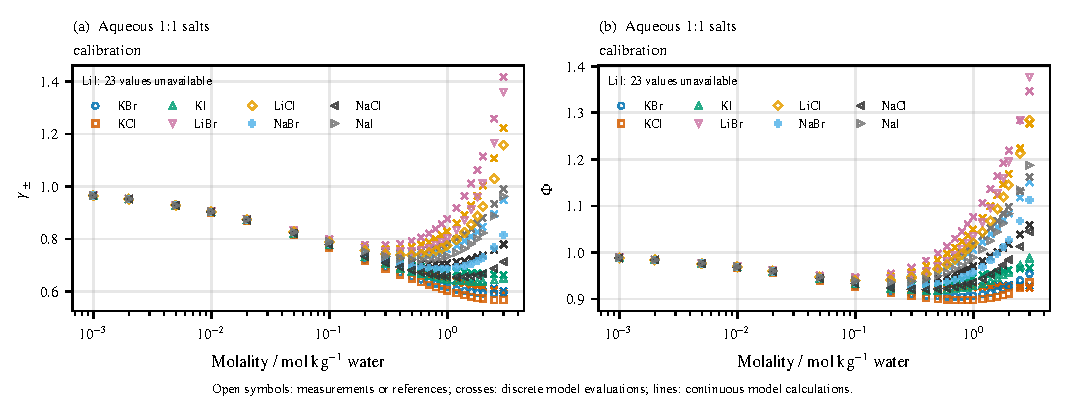
\includegraphics[page=1,width=0.94\linewidth]{F11-aqueous-electrolytes}
\caption{Mean ionic activity coefficients (left) and practical osmotic coefficients (right) of eight lithium, sodium and potassium halides at 298.15~K against the evaluated values of Hamer and Wu, computed with the Figiel parameters~\citep{HamerWu1972,Figiel2025}.
Open symbols are the evaluated values and crosses this package's values; LiI is not computed because the source supplies no lithium/iodide interaction.
The parameters were fitted partly to these data, so the comparison is calibration-related.
NaCl permittivity alternatives and the Held salt series are in the Supporting Information.}
\label{fig:aqueous-data}
\end{figure}

% P:physical-14
Held et al.~\citep{Held2008} broaden the properties to density, vapor pressure, water activity and mean ionic activity across 19 salts and 45 source series.
The full gallery displays every series with its source-line and measured-marker roles.
Unresolved neighboring source curves and disagreements remain visible, and the reconstruction is partial.
A pooled percentage over sampled correlated pixels would not be an experimental accuracy statistic, so none is given.
The separate Held osmotic comparisons~\citep{Held2014} at 273.15 and 298.15~K add a bounded temperature comparison, with the inferred diameter convention described in the Supporting Information.
They do not establish general temperature transfer for all electrolytes.

% P:physical-15
The NaCl permittivity comparison in the full aqueous gallery links activity accuracy to another physical quantity.
With the Figiel parameters and ion-suppression relation unchanged, the low- and higher-molality activity AARDs are 4.39\,\% and 5.35\,\%.
Refitting one shared water--ion interaction to the 21 activity observations at or below 2~mol/kg gives 0.666\,\% in that fitted population but 18.2\,\% over the eight higher-molality observations.
The density--temperature and dipolar-perturbation alternatives give withheld AARDs of 13.8\,\% and 16.7\,\%, yet miss much of the observed dielectric decrement.
Their relative-permittivity AARDs are 21.0\,\% and 23.5\,\%, compared with 7.27\,\% for ion suppression.
A more favorable activity extrapolation therefore does not by itself justify adopting a permittivity relation.
The alternative forms retain ion and Born parameters fitted with another relation, while primary-table lineage and pointwise measurement uncertainty remain unverified for this dielectric population.



\subsection{Mixed brines: failed transfer and a conditional refit}
% P:physical-16
A binary-salt parameter fit does not automatically constrain the cross-composition behavior of a mixed brine.
At 298.15~K and 100~kPa, the unchanged Held and Figiel parameters~\citep{Held2014,Figiel2025} fail the comparison limit in every source and ionic-strength range of the NaCl--MgCl$_2$ and NaCl--CaCl$_2$ water-property comparison~\citep{rardIsopiesticDeterminationOsmotic1987a,robinsonPropertiesAqueousMixtures1966,dinaneWaterActivitiesOsmotic2003a}.
Figure~\ref{fig:brine-data} compares residuals of the practical osmotic coefficient for the isopiestic data and the water activity for the Dinane--Mounir data.
The failure applies to these published parameter sets; it does not show that the equations cannot describe mixed salts with other parameters.

\begin{figure}[pos=H]
\centering
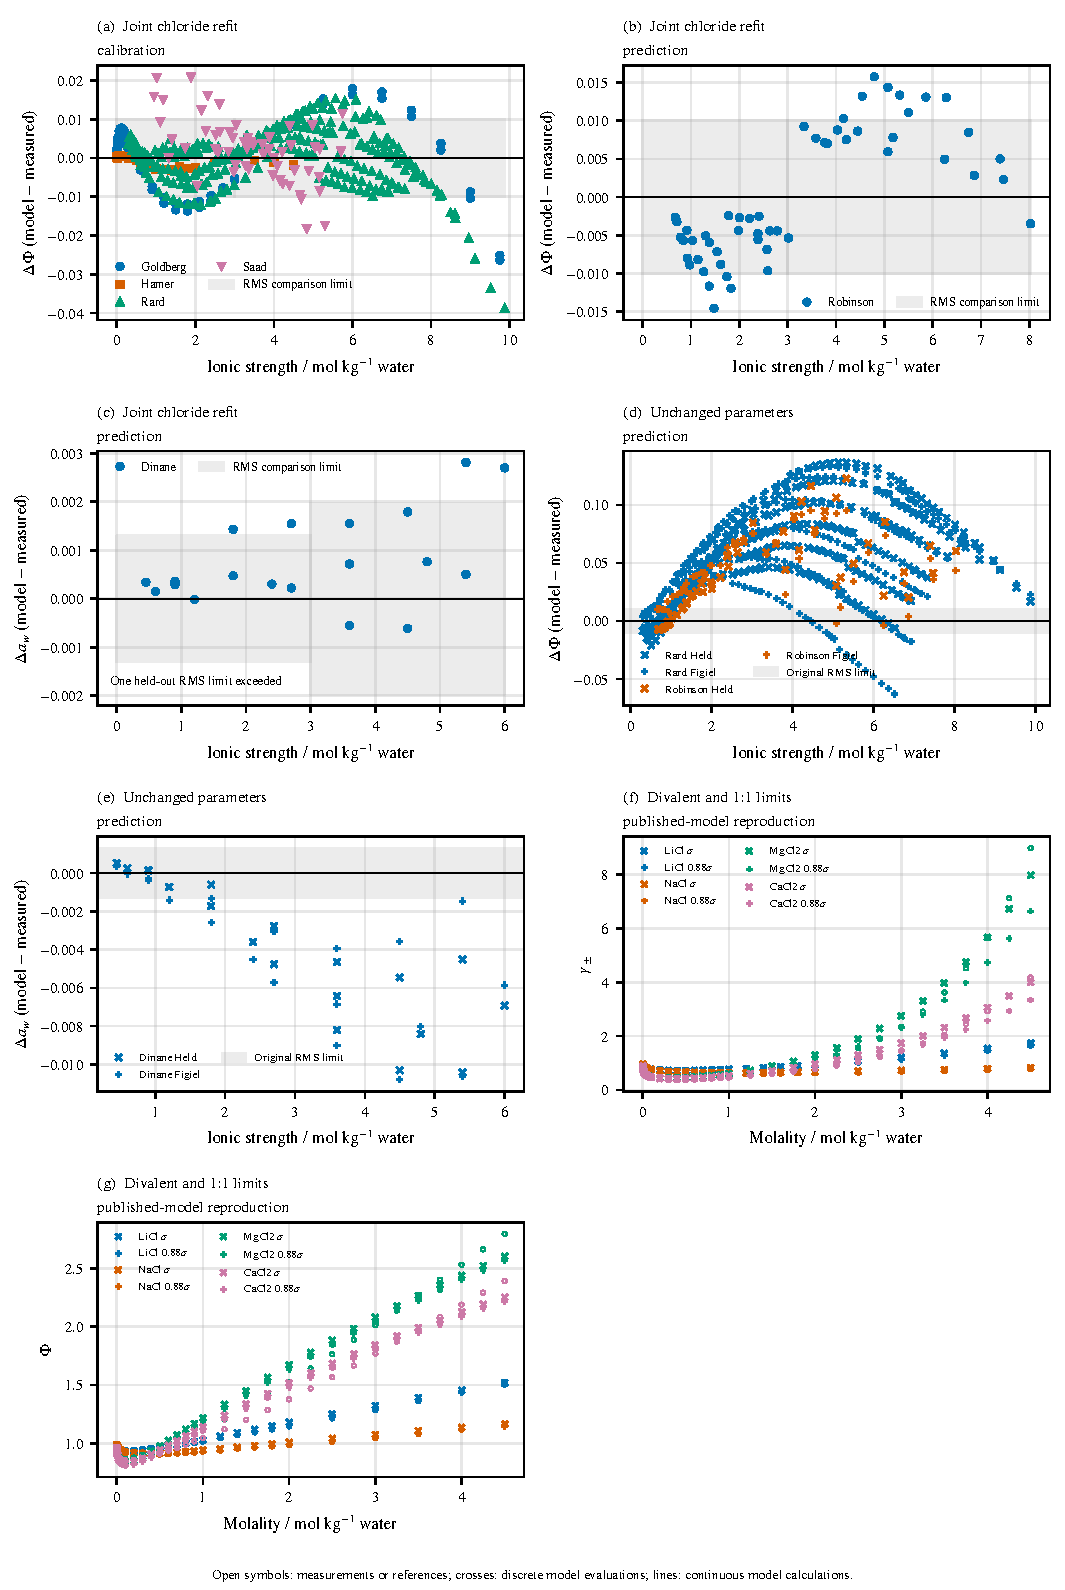
\includegraphics[width=0.91\linewidth,height=19cm,keepaspectratio]{F12-mixed-brines}
\caption{Residuals of mixed chloride brines at 298.15~K and 100~kPa against ionic strength.
Joint Figiel-form fit: (a) osmotic-coefficient training data, (b) withheld Robinson--Bower NaCl--CaCl$_2$ osmotic coefficients and (c) withheld Dinane--Mounir NaCl--MgCl$_2$ water activities.
Shaded bands in (a)--(e) show the corresponding RMS comparison limits, not pointwise measurement uncertainties; (c) uses the nominal source-agreement limit.
Unchanged published Held and Figiel parameters: (d) osmotic coefficients and (e) water activities of the same mixtures.
(f) Mean ionic activity and (g) osmotic coefficients of LiCl, NaCl, MgCl$_2$ and CaCl$_2$ with the Held strategy-2 parameters and the ion diameters $\sigma_i$ and $0.88\sigma_i$~\citep{Held2014}.}
\label{fig:brine-data}
\end{figure}

% P:physical-17
A joint Figiel-form fit adds binary NaCl, MgCl$_2$ and CaCl$_2$ osmotic data~\citep{HamerWu1972,goldbergEvaluatedActivityOsmotic1978}, Rard--Miller NaCl--MgCl$_2$ mixtures~\citep{rardIsopiesticDeterminationOsmotic1987a} and Saad NaCl--KCl--CaCl$_2$ mixtures~\citep{saadThermodynamicsMixedElectrolyte1980}, with the potassium parameters held fixed.
Its 443 training rows have RMS osmotic residual 0.00748.
The Rard--Miller data are calibration here, although they were predictions in the unchanged-parameter study.
Independent-source Robinson--Bower NaCl--CaCl$_2$~\citep{robinsonPropertiesAqueousMixtures1966} and Dinane--Mounir NaCl--MgCl$_2$~\citep{dinaneWaterActivitiesOsmotic2003a} mixtures supply the withheld data: RMS residuals are 0.00825 in osmotic coefficient and 0.00121 in water activity.
These values use the source data as printed.

% P:physical-18
Above an ionic strength of 3~mol/kg, the Rard--Miller training data, converted to water activity at the Dinane--Mounir compositions, differ from the Dinane--Mounir measurements by more than the original water-activity limit, so no model fitted to Rard--Miller can meet that limit.
After the fit, the limit for each Dinane--Mounir ionic-strength range was therefore set to the larger of the original limit and the disagreement between the two sources on the same rows, and applied to the existing fit without refitting.
To test the effect of rounding in the source tables, the comparison used the nominal data and 1466 perturbed versions that shift printed values by half a unit in their last printed digit.
The fit meets every withheld limit in 1466 of them; in the remaining one, which lowers every printed Dinane--Mounir value, the water-activity RMS for $I\le3$~mol/kg water is 0.001376 against a limit of 0.001352.
These perturbed data sets are sensitivity cases, not a probability distribution or new measurements.
The result supports a conditional description of the selected held-out mixtures at ionic strengths $I=0.45$--$8.03$~mol/kg water, with that explicit exception.
Above the held-out range, only training and reference checks are available: the magnesium-rich Rard--Miller training maximum $|\Delta\Phi|$ is 0.0388, and the separate pure-MgCl$_2$ reference check gives RMS 0.0289 and maximum 0.0376, exceeding the corresponding osmotic limits of 0.01 and 0.03.
The result does not demonstrate arbitrary simultaneous sodium/magnesium/calcium mixture accuracy or single-ion activities.
The corresponding Held-form fit is not offered as a mixed-brine description.

% P:physical-19
Divalent-salt comparisons also show why a diameter convention cannot be treated as a cosmetic input.
The paired Held strategy-2 screening declarations use $\sigma_i$ or $0.88\sigma_i$ and retain different errors for LiCl, NaCl, MgCl$_2$ and CaCl$_2$.
The full comparison reaches maximum absolute decadic errors of 0.131 for ionic activity and 0.0460 for osmotic coefficient over the paired population.
These maxima combine declared variants and are not an accuracy estimate for one adopted parameter set.
The divalent failures remain visible even where the monovalent coefficients are well represented.



\subsection{Mixed solvents, alcohol salts and solvation energies}
% P:physical-20
Solvent composition changes both the neutral mixture and the electrostatic environment of an ion.
Voltage-derived NaCl activity coefficients reported by Esteso et al.~\citep{Esteso1989}, Table~I, test fixed Figiel mixed-solvent parameters at 298.15~K across ethanol--water compositions.
The 123 comparisons give a pooled AARD of 6.35\,\%, with larger discrepancies in ethanol-rich mixtures than in the water-rich part of the population, although the trend is not monotonic.
Figure~\ref{fig:solvent-data} displays the composition dependence rather than replacing it by the pooled value.
The printed-digit comparison criterion is not a complete experimental uncertainty and supplies no claim that all excluded pointwise agreements are experimentally resolved failures.

\begin{figure}[pos=H]
\centering
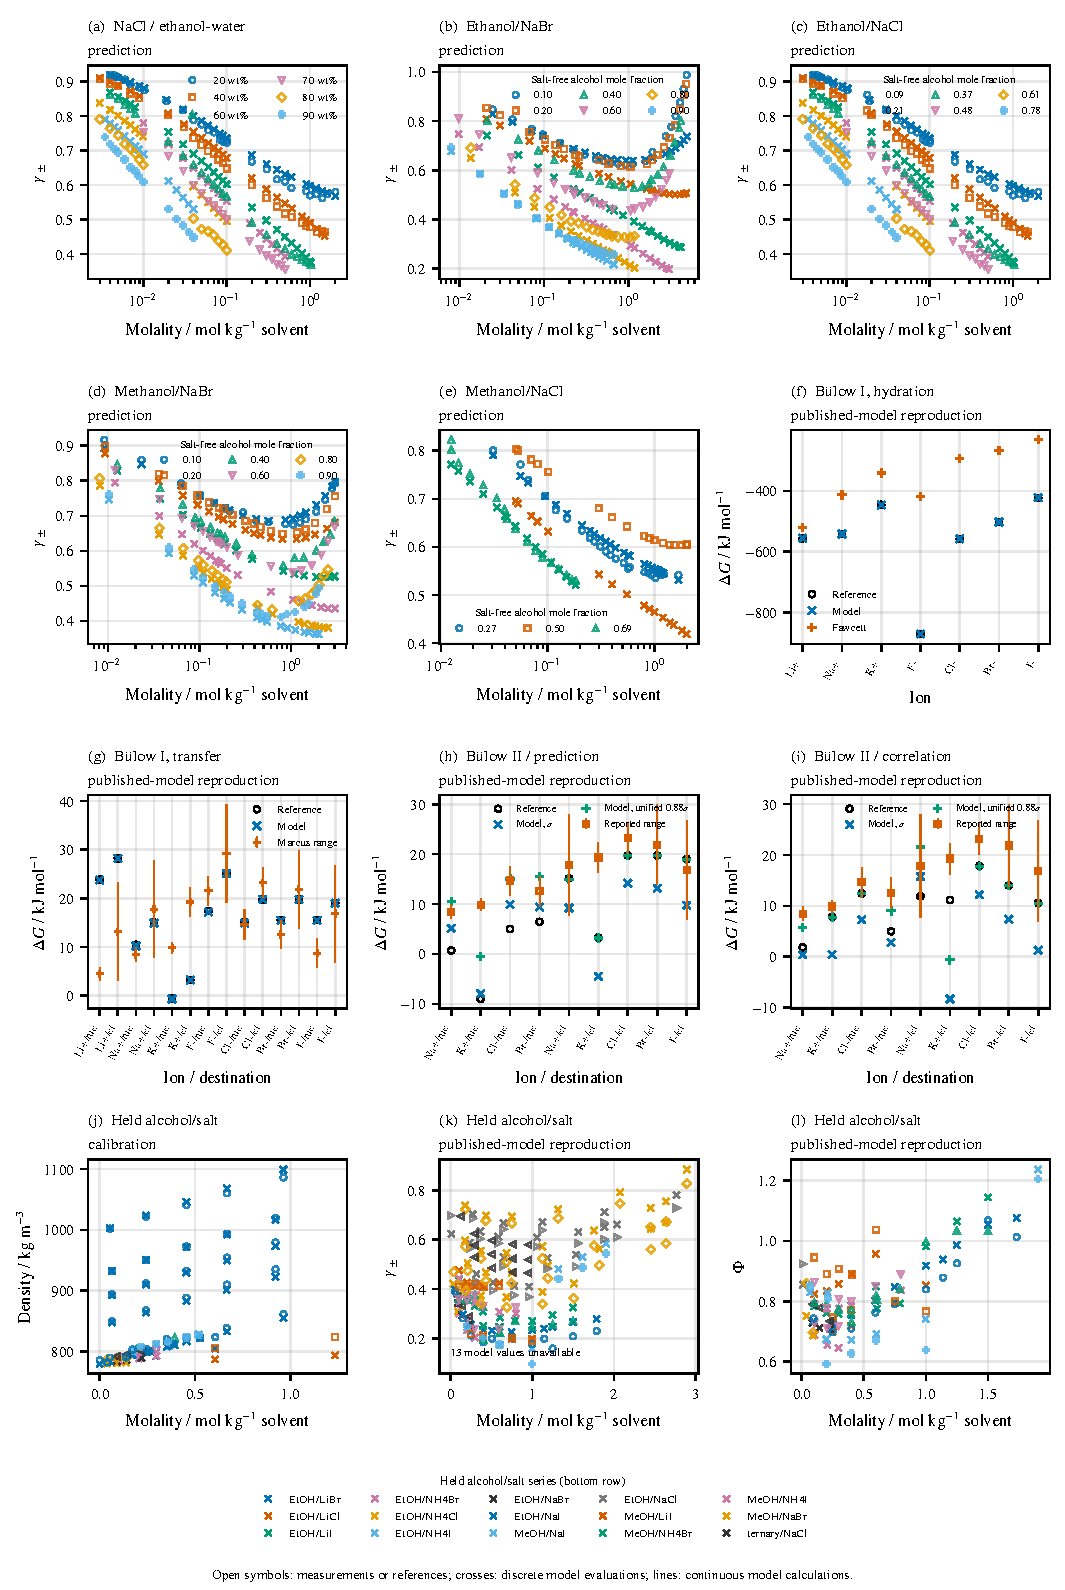
\includegraphics[width=0.91\linewidth,height=19cm,keepaspectratio]{F13-mixed-solvents-solvation}
\caption{Mixed-solvent activity, single-ion solvation and alcohol/salt properties constrain different parts of an electrolyte model~\citep{Esteso1989,Figiel2025,Bulow2020,Bulow2021,Held2012}.
Panels distinguish fixed-parameter prediction, calibration and published-model reproduction.
The Esteso and Figiel ethanol--NaCl observations overlap; reference ranges for single ions retain their conventions, and source-model bars remain separate from physical reference values.
}
\label{fig:solvent-data}
\end{figure}

% P:physical-21
The Figiel water--methanol and water--ethanol comparisons~\citep{Figiel2025} are fixed-parameter mixture predictions for NaCl and NaBr.
The NaBr parameters inherit pure-solvent activity fitting, so this classification does not establish independence from model development.
The four selected interior populations have dimensionless coefficient RMS differences from 0.0435 to 0.153.
Their primary-source lineage and measurement uncertainty are incomplete, and no independent-validation threshold is supplied.
The ethanol--NaCl population duplicates the Esteso observations, so displaying it under another model comparison does not add an independent dataset.
Excluded endpoints and the source limitations are preserved in the full table.

% P:physical-22
Ion hydration and solvent-transfer energies add another observable family~\citep{Bulow2020,Bulow2021}.
The figures compare model bars separately from the conventional single-ion reference values and ranges.
They show which diameter interpretation reproduces the paper calculations and where the transfer differs from those references.
Single-ion free energies depend on the adopted convention and are not convention-free direct measurements.
Agreement within the reading interval of a published model bar therefore tests model translation, not an independent hydration experiment.
The inferred $0.88\sigma_i$ diameter and the separation of correlated and predicted transfer populations remain explicit.

% P:physical-23
Alcohol/salt data from Held et al.~\citep{Held2012} add solution density, osmotic coefficient and derived ionic activity in methanol and ethanol.
The source parameters are solvent-specific and fitted to density and osmotic observations.
Derived ionic activities do not constitute an independent second osmometric experiment.
The direct tabulated comparisons miss the adopted printed-resolution criteria, while agreement with sampled source curves varies by property.
The source solvent-caption correction and the unresolved differences limit the interpretation to these declared calibration and reproduction comparisons.
They do not establish general salt transfer between water and alcohols.



\subsection{Electrolyte and reacting liquid splits}
% P:physical-24
The water/ethanol/isobutanol/NaCl comparison uses the Khudaida source parameters~\citep{Khudaida2026} for eight measured tie lines, solved at 293.15~K and 100~kPa with nominal 5~wt\% salt.
Each measured phase is expressed on a four-component formula basis, with NaCl counted as a formula unit rather than as two independent species fractions.
The mean absolute difference over the four coordinates of both phases is 0.0111 in mole fraction.
Figure~\ref{fig:reacting-data} shows the salt coordinates beside the solvent projection, preventing a favorable ternary projection from concealing salt-partition errors.
The adopted correlation-scale comparison is not agreement within measurement uncertainty, and the coordinate count is not a count of independent tie-line observations.
The manufactured feeds define the calculation without using measured endpoints as solver starts.

\begin{figure}[pos=H]
\centering
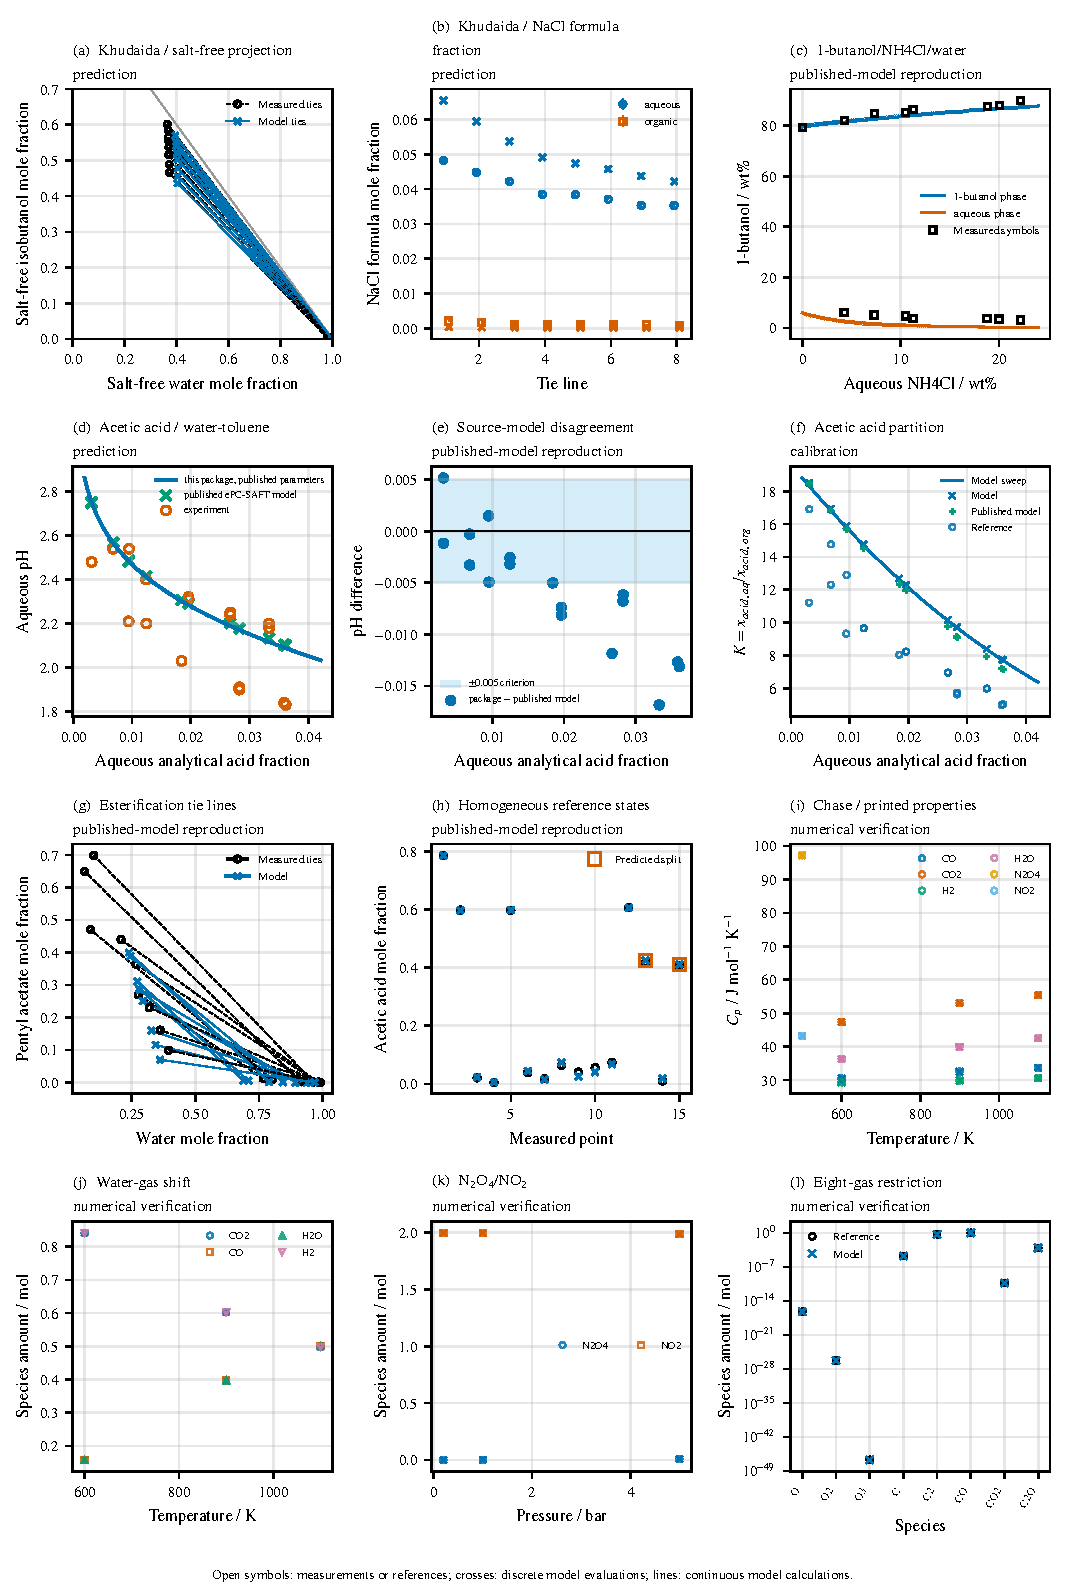
\includegraphics[width=0.91\linewidth,height=19cm,keepaspectratio]{F14-lle-reacting}
\caption{Liquid-split and reacting comparisons preserve the distinction between measured phases, source-model lines and numerical references~\citep{Khudaida2026,Held2014,Ascani2022pH,Ascani2023,Senina2022,Belov2023}.
The salted tie-line projection has a separate NaCl-coordinate panel; acid pH is paired with molecular partitioning; esterification retains incorrect phase counts.
The ideal-gas thermochemical and reaction-amount panels are numerical verification.
}
\label{fig:reacting-data}
\end{figure}

% P:physical-25
The 1-butanol/NH$_4$Cl/water comparison~\citep{Held2014} has a different reference role.
Its reference is a digitized published model line, not an additional set of measured tie lines.
The maximum selected butanol mass-percentage difference is 0.432 percentage point with the declared inferred ion-diameter convention.
That agreement establishes bounded reproduction of the calibrated source model.
The full table keeps this population separate from the measured Khudaida coordinates.

% P:physical-26
Acetic acid dissociation and water autoprotolysis coupled to water/toluene liquid splitting test reaction references and phase equilibrium together~\citep{Ascani2022pH}.
The aqueous pH predictions have MAE 0.146 pH unit at 19 measured compositions.
Only seven source-model pH values meet the separate 0.005-unit reproduction criterion, with maximum absolute difference 0.0169 pH unit.
The molecular-acid partition coefficient is $K=x_{\mathrm{acid,aq}}/x_{\mathrm{acid,org}}$, distinct from the reaction equilibrium constant.
It gives 47.8\,\% AARD against the measured partition population, whose acid--organic interaction belongs to a calibration family with unresolved exact overlap.
The pH and partition results therefore support different conclusions; a relatively close pH curve does not establish accurate distribution of acid between the liquids.
Organic trace-ion amounts and organic pH remain unresolved, and no charged phase-stability conclusion follows.

% P:physical-27
Reactive esterification adds acetic acid, 1-pentanol, pentyl acetate and water at 318.15~K~\citep{Ascani2023,Senina2022}.
The selected homogeneous and tie-line composition RMS differences are 0.00738 and 0.0829, respectively.
The reaction constant partly inherits calibration to the measured system, so these are published-model/calibration-related physical comparisons.
The wrong predicted phase counts for measured homogeneous points 13 and 15 remain in the interpretation.
Satisfying the reaction residual at a computed split does not correct a wrong phase count or make the tie-line error small.
The gas-reaction panels in the same gallery check ideal thermochemistry and equilibrium amounts against reference calculations~\citep{linstromNISTChemistryWebBook1997,Belov2023}; they are numerical verification and add no physical reacting-liquid validation.



\subsection{Reactive amines: calibration does not establish pressure accuracy}
% P:physical-28
The MDEA examples expose a substantial limit of transferring a fitted electrolyte description to reacting vapor--liquid equilibrium.
For the Wangler formulation~\citep{Wangler2018}, ten osmotic observations at 273 and 313~K determine a water--protonated-MDEA interaction under two declared ion-dispersion conventions, S0 and S1.
The calibrated osmotic AARDs are between 1.43\,\% and 2.65\,\% across temperature and convention.
The subsequent pressure comparison at 303~K and 60~wt\% MDEA was not used in that fit.
It gives 96.2\,\% and 89.6\,\% AARD for the fitted S0 and S1 variants at the three measured pressures.
Figure~\ref{fig:amine-data} shows both the fitted coefficients and failed pressure transfer.
The cause remains an unresolved model-reading or parameter-transfer discrepancy; this evidence does not establish a general defect of every MDEA formulation and supplies no MEA accuracy result.

\begin{figure}[pos=H]
\centering
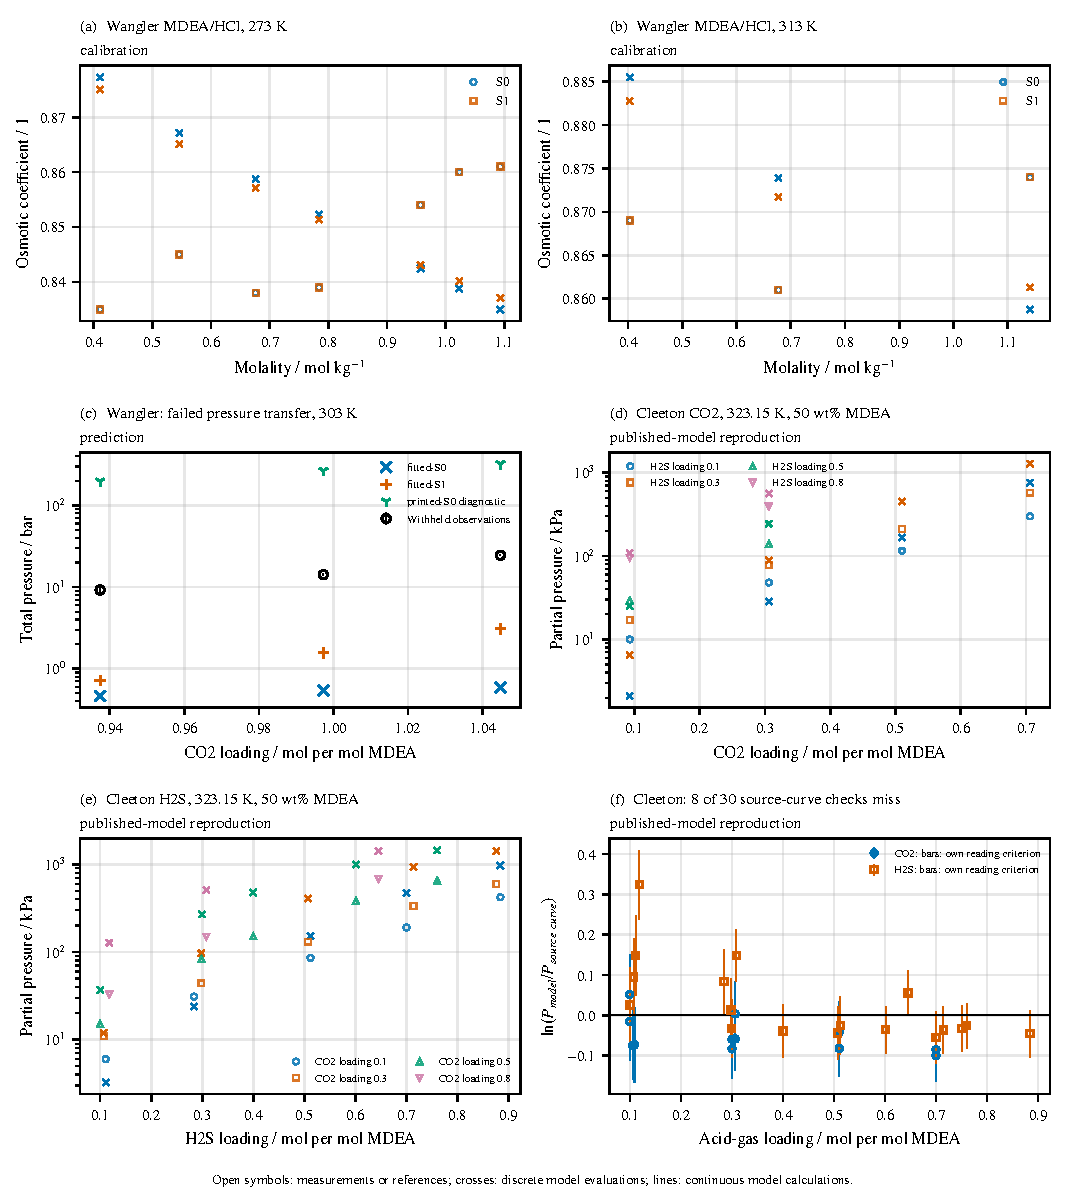
\includegraphics[width=0.92\linewidth,height=18cm,keepaspectratio]{F16-reactive-amines}
\caption{Reactive MDEA comparisons retain unsuccessful transfer~\citep{Wangler2018,Cleeton2020}.
The Wangler panels separate osmotic calibration from pressure prediction at withheld conditions.
The Cleeton panels separate measured partial-pressure comparisons from published-curve reproduction, including eight source-curve misses and the methane omission.
Grey markers (printed-S0) use the Wangler parameters as printed in the source and are shown as a diagnostic, not a fit.}
\label{fig:amine-data}
\end{figure}

% P:physical-29
The Cleeton comparison~\citep{Cleeton2020} recalculates competitive CO$_2$/H$_2$S absorption in 50~wt\% MDEA at 323.15~K with inherited source parameters and no refit to the selected partial pressures.
The primary published-curve reading meets its digitization criterion at 22 of 30 points, leaving eight curve misses.
Ordinary AARDs against the measured CO$_2$ and H$_2$S partial pressures are 64.4\,\% and 143.7\,\%.
These differ from a symmetric relative-deviation statistic, which gives less weight to large overprediction and cannot be reported under the same AARD definition.
The declaration omits methane present in the source record and uses the stated inferred ionic-diameter convention.
It is a bounded published-model replay with large physical discrepancies, rather than an absorption-prediction success.

\section{Numerical verification and solution limits}
\label{sec:verification}
% P:verification-01
Numerical verification isolates errors in equations, closures, derivatives and solved-state transport from the physical discrepancies in Section~\ref{sec:physical}.
Table~\ref{tab:verification} summarizes representative checks with their reference and unit.
Cross-code comparisons use matched parameters, equations and constants; finite-difference comparisons use declared directions and step refinement on the same smooth branch.
An observed code difference without an independent reference is not automatically an error of one code.
Unless stated otherwise, the comparisons use FeOs~0.10.1, Clapeyron.jl~0.6.29 and teqp~0.23.2; the five-code propane comparison uses the surveyed source versions in Table~\ref{tab:software}.

\begin{table}[pos=htbp]
\centering\small
\caption{Numerical verification on the stated populations. Bounds are rounded outward. Ratios to a criterion are dimensionless and do not represent physical model errors.}
\label{tab:verification}
\begin{tabularx}{\linewidth}{@{}p{0.37\linewidth}p{0.29\linewidth}X@{}}
\toprule
Quantity / population & Reference & Maximum difference or ratio \\
\midrule
Propane saturation pressure, 300~K & Five matched codes & $1.10\times10^{-9}$ relative \\
Propane critical candidate & FeOs; teqp & $8.3\times10^{-11}$; $8.3\times10^{-15}$ relative \\
First solved-state actions, bubble and liquid split & Clapeyron implicit derivatives & $3.40\times10^{-10}$ relative \\
Electrolyte liquid compositions, 8 feeds & Matched constant-permittivity Clapeyron flash & $4.62\times10^{-9}$ mole fraction \\
Direct Born term, aqueous NaCl & Matched constants, Clapeyron; FeOs & $3.41\times10^{-16}$; $8.21\times10^{-12}$ relative \\
Dipole contribution, 8 states & teqp & $10^{-15}$ relative \\
Pressure-specified caloric actions, 36 comparisons & Refined differences & 0.34 of criterion \\
Selected second / third solved actions & Refined lower actions; analytic isomerization & $5.92\times10^{-4}$ / $2.45\times10^{-4}$ of criterion \\
Electrolyte fitting columns, 3\,167 & Refined differences & 0.0145 of allowance \\
Two-reaction ionic extraction feed actions & Finer of two central-difference steps & $3.52\times10^{-6}$ relative \\
Selected density roots, 704 requests & Frozen / separate scan & $1.56\times10^{-11}$ / $1.60\times10^{-11}$ relative \\
Same density requests, pressure closure & Defining pressure equation & $2.19\times10^{-13}$ reduced residual \\
Manufactured reacting caloric comparisons & Identities, refined differences, quadrature & 0.0952 of criterion among numerical ratios \\
Manufactured least-squares / minimax coordinates & Known parameters / analytic optimality & $7.35\times10^{-11}$ / $6.01\times10^{-11}$ absolute \\
\bottomrule
\end{tabularx}
\end{table}

\subsection{Shared equations across independent implementations}
\label{sec:cross-code}
% P:verification-02
Propane saturation at 300~K with Gross--Sadowski parameters~\citep{Gross2001} gives a common case for this package, FeOs, Clapeyron.jl, teqp and ThermoPack.
The pressure agrees within the bound in Table~\ref{tab:verification}; representative numerical values appear in the Supporting Information for independent implementation checks.
The critical and neutral bubble/dew comparisons in the full envelope gallery are discrete numerical comparisons, separate from the native continuation line.
Pressure--enthalpy and pressure--entropy comparisons with FeOs use the same manufactured ideal-gas thermal records and common caloric increments, avoiding a false comparison between different reference enthalpies.
The shared-model checks do not assess experimental caloric accuracy.

% P:verification-03
A direct Born comparison for aqueous NaCl matches electrostatic constants before evaluating the code difference.
The remaining differences are much smaller than the discrepancy obtained with unmatched constants.
The optional dipole term likewise agrees with teqp on selected fixed neutral states~\citep{Gross2006,bellImplementingEquationState2022}.
The corrected solvation-shell Born term and ion-suppression relation have derivative/identity checks but no independent same-equation value implementation in this comparison.
That gap is distinct from the measured-data errors of those parameterizations.

% P:verification-04
For the eight water/ethanol/isobutanol/NaCl feeds at 293.15~K and 100~kPa, constant permittivity and the direct Born term define a deliberately matched electrolyte model.
Clapeyron.jl then reproduces the package's phase mole fractions within $4.62\times10^{-9}$ from the compared starts (Fig.~\ref{fig:electrolyte-lle}a).
Restoring composition-dependent permittivity produces a larger cross-code discrepancy.
A termwise probe places the difference in solvent Debye--H\"uckel chemical potentials: Clapeyron.jl~0.6.29 omits their inverse-Debye-length dependence through solvent composition while its permittivity gradient itself agrees with differences.
Supporting Information Section~\ref{sec:si-probe} gives the isolating comparisons.
The unmatched variant therefore supplies a diagnosed limit of the comparison, not a successful verification of either returned split against the other.

\begin{figure}[pos=H]
\centering
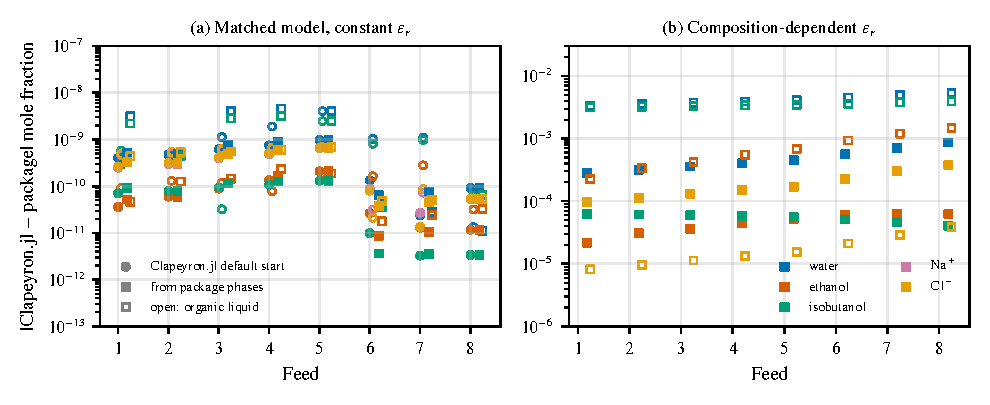
\includegraphics[width=\linewidth]{electrolyte-lle}
\caption{Matched and unmatched electrolyte code comparisons answer different questions (numerical verification).
(a) Constant-permittivity phase mole fractions agree below the $10^{-8}$ comparison line for both starts.
(b) Composition-dependent permittivity yields larger differences associated with the solvent Debye--H\"uckel derivative; the default comparator start returns no valid split.
Filled and open markers denote the water-rich and organic liquids, with the ionic fractions coincident by charge neutrality.
The model-convention and derivative probe is described in Supporting Information Section~\ref{sec:si-probe}.}
\label{fig:electrolyte-lle}
\end{figure}



\subsection{Derivative accuracy and reference resolution}
\label{sec:derivative-verification}
% P:verification-05
The 36 pressure-specified residual enthalpy, entropy and heat-capacity actions cover orders one to three for four electrolyte records, along declared temperature, pressure and composition directions.
Their criteria scale with the sum of the magnitudes of directional parts, preserving a meaningful scale when high-order terms cancel.
Every error is below 0.34 of its criterion (Fig.~\ref{fig:derivatives}a).
At third order the errors approach the estimated uncertainty of the refined references, so the observed agreement is reference-limited.
Independent implicit derivatives from Clapeyron.jl and FeOs test selected solved bubble-point and liquid--liquid responses separately from the package's own central differences (Fig.~\ref{fig:derivatives}b).

\begin{figure}[pos=H]
\centering
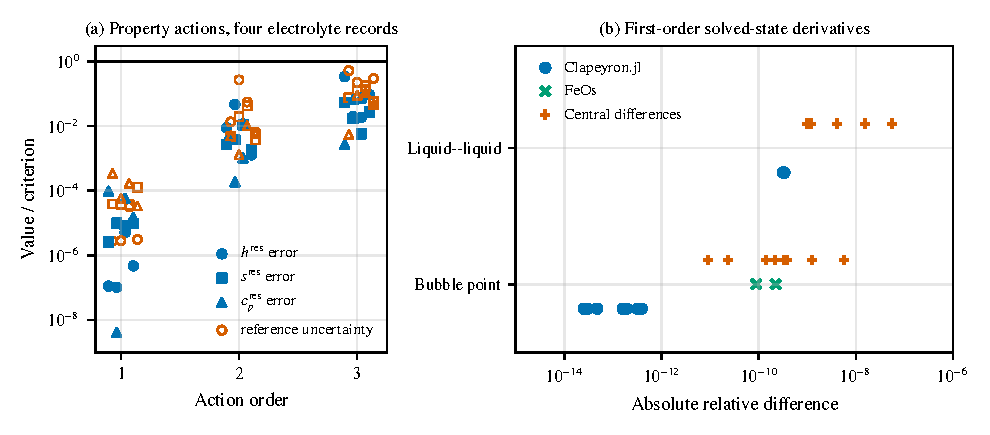
\includegraphics[width=\linewidth]{derivatives}
\caption{Derivative errors must be interpreted with the resolution of their references (numerical verification).
(a) Pressure-specified caloric-action errors divided by their criteria (filled), with refined-reference uncertainty on the same scale (open), grouped by order and parameter record.
(b) Selected first-order solved-state derivatives against independent implicit derivatives and the package's central differences.
Each point identifies an observable and physical direction; it is not an all-direction guarantee.}
\label{fig:derivatives}
\end{figure}

% P:verification-06
Second- and third-order solved actions use neutral ternary, single-phase electrolyte and manufactured reacting branches.
Refined lower-order actions and analytic isomerization values provide their references, with normalized errors shown in Table~\ref{tab:verification}.
Shared lower-order differentiation can conceal a common error and therefore does not replace the independent analytic comparisons.
The reacting caloric set contains 12\,975 comparisons, of which 122 have no numerical error-to-criterion ratio.
Among those with ratios the largest is 0.0952; all defining criteria are met.
Quadrature of equilibrium heat capacity and its temperature derivative recovers independently solved enthalpy and heat-capacity increments, providing a consistency check on the reference and reaction chains of Section~\ref{sec:derivatives}.
The chemistry is manufactured, so none of these counts is a calorimetric validation population.



\subsection{Balances, root selection and fitting calculations}
\label{sec:balances}
% P:verification-07
The density checks comprise 704 branch-specific requests evaluated in three modes, rather than three independent physical populations.
Selected densities agree with frozen references and a separate scan within the bounds in Table~\ref{tab:verification}, and reduced pressure residuals stay below $10^{-12}$.
The scan and selected-root routines share their equation evaluator.
Nested-grid agreement tests numerical root location on the finite searched domain, with no proof of complete enumeration.

% P:verification-07b
Given only the feed, temperature and pressure, explicit phase discovery returns the phases of the package's own declared solve for five neutral states: water/isobutanol with two liquids at 293.15~K and 100~kPa; water/ethanol/isobutanol with vapor and two liquids at 364.2~K and 100~kPa; single liquids of equimolar water/ethanol and of water with an isobutanol mole fraction of 0.005 at 293.15~K and 100~kPa; and a manufactured equimolar ternary with three liquids at 300~K and 10~MPa.
Across these states, the largest absolute composition difference is $1.94\times10^{-14}$, and the largest difference in $G/(RT)$, scaled by the larger of unity and the reference magnitude, is $7.67\times10^{-15}$.
For the equimolar water/hexane liquid at 300~K and 100~kPa (Fig.~\ref{fig:search-envelope}, top), the two stationary trials from near-pure liquid seeds agree with the FeOs stability analysis, and the discovered liquid split with the FeOs flash, within $1.58\times10^{-11}$ in mole fraction and $8.81\times10^{-11}$ in relative density after refinement of the FeOs results.
These are finite-point numerical comparisons, not physical validation or a global stability certificate.

% P:verification-07c
Charged trials check the condensed-phase condition of Section~\ref{sec:stability}: under a density-independent permittivity a charged trial point is admitted only as a mechanically stable density root on the liquid side of its own composition's pressure loop, and every seed and supplied point reported here returns the admission or unavailability that this condition predicts for it.
All four charged seeds are admitted for the water/ethanol/isobutanol/NaCl split at 293.15~K and 100~kPa, and both are admitted for the aqueous NaCl liquid at 298.15~K and 100~kPa.
For the reacting aqueous MEA/\ce{CO2} declarations at 318.15~K, a bubble at its solved pressure of 7.39816~kPa and a flash and a liquid at 5.9185286 and 8.8777929~kPa, three of four charged seeds are admitted; the remaining seed is unavailable because its only density root lies on the vapor side of its composition's pressure loop.
Trial points supplied by composition and density, rather than found by minimization, are admitted at the aqueous and salt-rich liquid roots of aqueous NaCl at 298.15~K and 100~kPa, whereas the aqueous vapor root, an off-root salt-rich point and a loop-less MEA point remain unavailable under the same condition, with no reported tangent-plane distance.
Unavailable points are never reclassified as stable because a distance could not be evaluated.
Among the reconstructed trial points, the largest normalization and charge defects are $2.64\times10^{-16}$ and $6.94\times10^{-18}$, both against a criterion of $10^{-12}$, and the largest difference between a trial's tangent-plane distance and the value implied by its balance multipliers, divided by $RT$, is $1.95\times10^{-13}$ against $10^{-10}$.
Discovery returns two liquids for the electrolyte split and one liquid each for the aqueous NaCl and reacting liquid declarations, the same phase counts as their declared solves.
For the MEA flash, whose declared two-phase solve succeeds, the search finds resolved descent but admits no declaration of lower Gibbs energy, so discovery stops explicitly without returning a phase set (Algorithm~\ref{alg:discovery}).
No discovery is requested for the free-pressure bubble.
These admission checks establish neither successful MEA flash discovery nor global stability; the estimated numerical uncertainty is not a rigorous bound.

% P:verification-08
A nine-species two-reaction lithium/sodium extraction declaration tests coupled balance and action calculations at 298.15~K and 101.325~kPa.
Over 67 central, perturbed and repeated solves, conserved-moiety defects are below $1.43\times10^{-14}$~mol and charge defects below $8.67\times10^{-15}$~mol.
The finer-step feed derivatives agree with exact actions within $3.52\times10^{-6}$ relative.
The pseudo-components and reaction constants are calibrated assumptions, so these results verify the declared numerical equations and supply no measured extraction accuracy.
The zero-inventory checks separately verify absent-species removal and allowed on-face calculations.
\todo{Insert numerical results for the reacting MEA flash family.}

% P:verification-09
Manufactured least-squares and minimax problems test known-parameter recovery and optimality equations, with the coordinate errors in Table~\ref{tab:verification}.
The electrolyte column comparison tests the full chain through density, reference and held Born diameter, rather than differentiating the final residual formula alone.
These checks establish numerical behavior on their declared observations; they do not imply identified physical ion parameters.
The process examples in Section~\ref{sec:applications} then test transport of the same native values and derivatives into an external equation-oriented model.

\section{Computational cost}
\label{sec:performance}
% P:performance-01
The cost of a request depends on what it returns, so cost is compared by operation and only where two codes return the same values.
Five operations are distinguished (Table~\ref{tab:cost}): a property bundle of a state at fixed density; a state at fixed pressure, which adds density closure; a declared equilibrium solve; an explicit phase discovery; and first-order actions on a state that is already solved.
FeOs~0.10.1~\citep{rehnerFeOsOpenSourceFramework2023} and Clapeyron.jl~0.6.29 under Julia~1.13.1~\citep{walkerClapeyronjlExtensibleOpenSource2022} supply the comparator implementations.
A timing comparison requires scaled property differences below $10^{-8}$, relative density-closure differences below $10^{-10}$, relative equilibrium pressure and density differences below $10^{-7}$, and absolute composition and phase-fraction differences below $10^{-8}$.
Every timed comparator case met these criteria.
Initial model construction, process startup, Julia compilation, warmups and request transport are excluded.
The central-difference timings include constructing shifted parameter records and mixtures and re-solving the displaced states.
Each code runs in its own persistent worker process, and two independent package workers bracket the FeOs and Clapeyron.jl workers in alternating order over three repetitions.
Each worker's time is the median of its three block medians of warm calls.
Each paired ratio divides a package block median by the comparator block median from the same repetition; the reported ratio is the median of the six such ratios, two package workers by three repetitions, with their full range beside it.
That range describes observed spread, not a confidence interval.
The ratios compare the calls each code exposes for the same result, not equal algorithms, and they hold for one host.

% P:performance-02
The marginal cost of exact derivatives is reported as actions on a solved state: the time of the first-order actions after a central solve, against the time of central differences that re-solve the state at shifted inputs.
The ethanol--butane bubble-point actions return pressure and vapor composition along temperature, the binary interaction parameter and the two ethanol association parameters; the water--pentanol actions return the water mole fraction of each liquid and the water-rich phase amount along temperature and the binary interaction parameter.
That ratio excludes the central solve, which both routes need, so it is not a speedup of a whole calculation or a comparison with another code's implicit derivatives.
No comparator was timed on charged or reacting cases, and no comparative cost claim is made for them.

% P:performance-03
The fixed-density bundle uses propane at 300~K and 500~mol\,m$^{-3}$; density closure uses a changing-pressure sequence of liquid propane states at 300~K near 1.9974~MPa.
Declared equilibrium cases are propane saturation at 300~K, equimolar ethanol--butane bubble pressure at 373.15~K, and an equimolar water--pentanol liquid split at 298.15~K and 101.3~kPa.
Explicit discovery uses equimolar methane--ethane at 190~K and 1~MPa, a two-phase point at which all three codes return the same phases.
At another methane--ethane point the codes did not return the same state quantities, so that point was not timed and the discovery ratio does not extend to other points.
Measurements used an AMD Ryzen 9 5900XT with 32 logical CPUs, workers pinned to logical CPU~31 with one numerical thread each, and one-minute load averages of 3.37--3.95 before and after the selected blocks; a block was admitted only when the load average was below 4 before and after it.
Each worker supplied 75 samples for each property-bundle and declared-equilibrium case, 15 for density closure and discovery, and 30 for each exact-action or central-difference set, across three blocks.
The electrolyte calculation was timed for the package only: the eight water/ethanol/isobutanol/NaCl feeds of Section~\ref{sec:cross-code} (Fig.~\ref{fig:electrolyte-lle}a) at 293.15~K and 100~kPa with constant permittivity, with 15 samples per worker.
The first package worker's median was 154.6~ms for the whole eight-feed set, with block medians from 154.6 to 156.6~ms; the second package worker gave 160.5~ms, from 158.5 to 164.4~ms.
One propane-saturation block exceeded the load-average limit, so it was excluded and the complete saturation operation was repeated with all workers; the selected measurements contain 102 blocks and 1590 samples.

\begin{table}[pos=htbp]
\centering
\caption{Package time divided by comparator time for value-matched operations, and exact-action time divided by the package's central-difference time on the same solved state: median [minimum, maximum] of six paired block ratios.
Values below unity mean less package or exact-action time; the density-closure comparison with Clapeyron.jl is a tie within the observed spread.}
\label{tab:cost}
\small
\begin{tabularx}{\linewidth}{@{}Xcc@{}}
\toprule
Operation and case & Package / FeOs & Package / Clapeyron.jl \\
\midrule
Property bundle at fixed density, propane & 0.2147 [0.0690, 0.2346] & 0.5058 [0.4370, 0.8999] \\
Density closure at fixed pressure, liquid propane & 0.2728 [0.2447, 0.4857] & 0.8457 [0.5677, 1.469] \\
Declared equilibrium: propane saturation & 7.260 [5.726, 7.524] & 4.514 [4.091, 5.229] \\
Declared equilibrium: ethanol--butane bubble point & 1.940 [1.883, 2.106] & 0.8189 [0.7067, 0.8714] \\
Declared equilibrium: water--pentanol liquid--liquid split & 0.2841 [0.2828, 0.2897] & 1.957 [1.492, 2.018] \\
Explicit phase discovery: methane--ethane & 32.50 [30.14, 32.84] & 11.76 [10.40, 15.89] \\
\midrule
\multicolumn{3}{@{}l}{Exact first-order actions / package central differences, central solve excluded} \\
Ethanol--butane bubble point & \multicolumn{2}{c}{0.02766 [0.02654, 0.05074]} \\
Water--pentanol liquid--liquid split & \multicolumn{2}{c}{0.009577 [0.008246, 0.01233]} \\
\bottomrule
\end{tabularx}
\end{table}

% P:performance-04
The property bundle costs less than either comparator, and density closure costs less than in FeOs and ties with Clapeyron.jl within the observed spread (Fig.~\ref{fig:cost}).
For the ethanol--butane bubble point and the water--pentanol split the package time lies between the two comparator times, whereas propane saturation takes 4.5 and 7.3 times and explicit discovery 11.8 and 32.5 times the Clapeyron.jl and FeOs times.
These measurements do not isolate the causes: the codes differ in initialization, reuse of previous results, stopping rules and discovery method, and matching the returned state does not establish equivalent phase-search coverage or a package-wide speed factor.
The two solved-state action ratios quantify marginal derivative cost only.

\begin{figure}[pos=htbp]
\centering
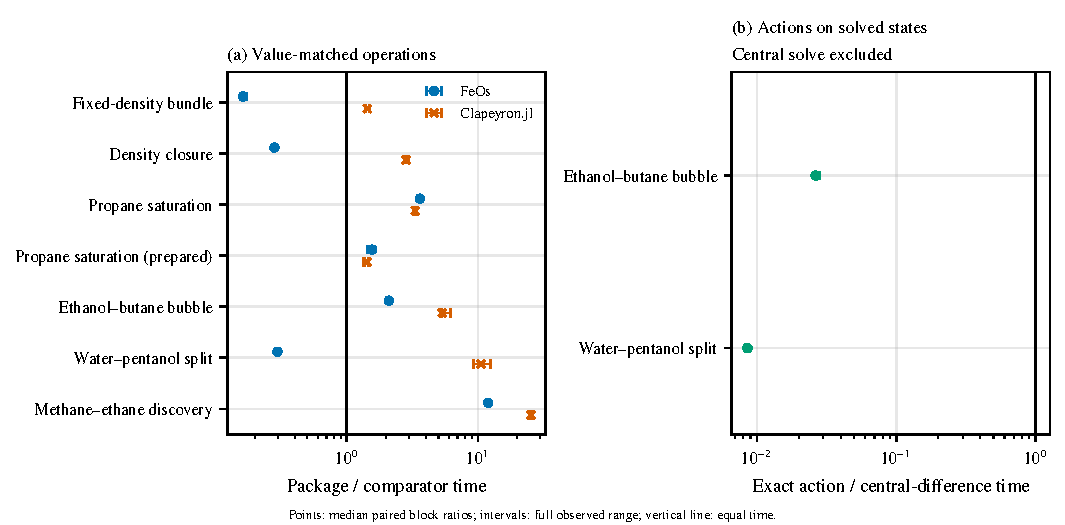
\includegraphics[width=\linewidth]{F6-computational-cost}
\caption{Value-matched computational costs.
(a) Package time over FeOs or Clapeyron.jl time for each operation; the fixed-density bundle and density closure use propane.
(b) Exact first-order action time over the package's central-difference time on an already solved state, excluding the central solve.
Points show medians and horizontal intervals the full ranges of six paired block ratios; the vertical line marks equal time, and points left of it mean less package time in (a) and less exact-action time in (b).
The electrolyte calculation has no comparator and is excluded.}
\label{fig:cost}
\end{figure}
\clearpage

\section{Use in engineering calculations}
\label{sec:applications}
\subsection{A local two-liquid settler optimization}
% P:applications-01
A water/ethanol/isobutanol/NaCl settler connects the equilibrium and action calculations to an equation-oriented process model.
At 293.15~K and 100~kPa, the external IDAES/Pyomo model~\citep{leeIDAESProcessModeling2021,hartPyomoModelingSolving2011} minimizes normalized isobutanol and salt use subject to at least 96.5\,\% ethanol recovery in the organic outlet.
The isobutanol and salt feed rates, as multipliers of their base values, are bounded from 0.85 to 1.15, and every property call stays on a declared local two-liquid branch with Khudaida source parameters~\citep{Khudaida2026}.
The compiled external functions return outlet species amounts and exact first and second feed derivatives from the common native equilibrium equations.
The outer process optimizer therefore receives the response of the full phase split, rather than a derivative at frozen phase composition.

% P:applications-02
Three starts converge to the same local process point, with the isobutanol feed raised to 1.0604 and the salt feed lowered to 0.9152 of their base values, a normalized objective of 1.97564 against 2 at the base design, and ethanol recovery at the specified constraint.
The largest stored stationarity norm is $3.666\times10^{-12}$, complementarity is below $9.10\times10^{-11}$ and component closure below $1.12\times10^{-16}$~mol/s.
All 1\,050 transported values and derivative entries equal the native values exactly.
Figure~\ref{fig:engineering} shows the outlets and the stored local stationarity values for this same calculation.
Transport equality tests the external-function connection; balance and optimality residuals test the solved model.
The calculation is nonreactive and fixed in temperature and pressure, so it supplies neither reactive extraction validation nor a global process optimum.

\begin{figure}[pos=H]
\centering
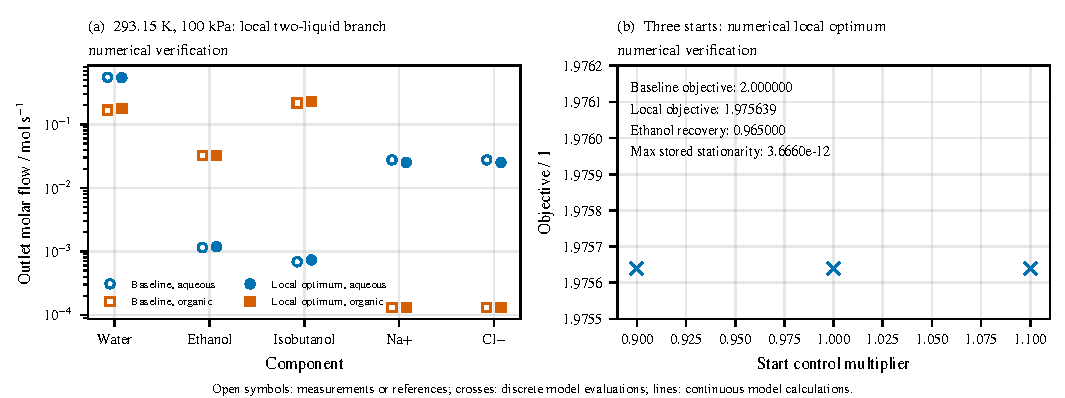
\includegraphics[width=0.96\linewidth]{F17-settler}\par
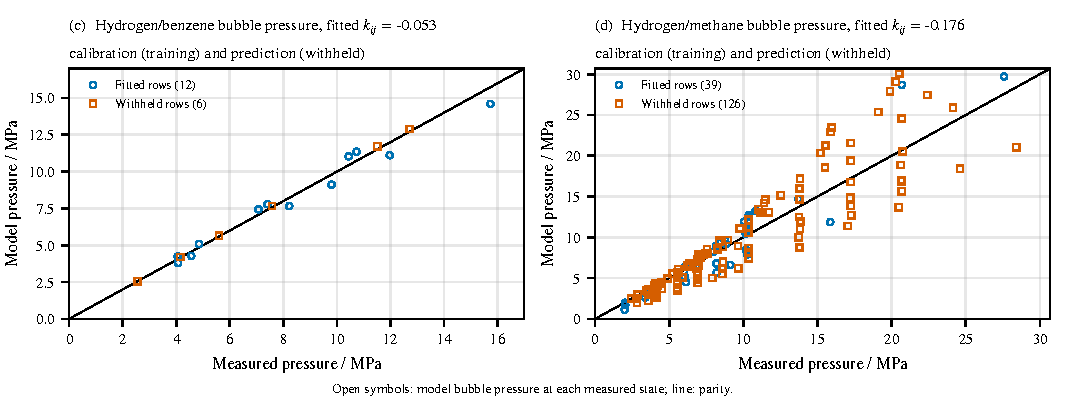
\includegraphics[width=0.96\linewidth]{F18-hda-hydrogen-pairs}
\caption{Engineering examples expose both numerical integration and parameter-domain limits.
Top: the fixed-condition Khudaida settler calculation shows outlet flows and local stationarity for the selected three-start calculation (numerical verification)~\citep{Khudaida2026}.
Bottom: hydrogen/benzene and hydrogen/methane bubble-pressure calibration and withheld prediction for pair parameters used in a two-flash example~\citep{Park1996,Benham1957,Sagara1972,Hong1981}.
}
\label{fig:engineering}
\end{figure}

\subsection{Hydrogen binary fits for a two-flash calculation}
% P:applications-03
A hydrodealkylation two-flash example uses hydrogen, methane, benzene and toluene to connect fitted pair parameters to an external phase-equilibrium model.
The external IDAES model owns its flash and smoothing equations, while the package supplies pressure-specified density, total enthalpy and component fugacity coefficients with exact derivatives.
Before any process result is interpreted, the hydrogen pair interactions must be supported by measured binary states at the conditions used.
Figure~\ref{fig:engineering} compares hydrogen/benzene and hydrogen/methane bubble pressures under zero and fitted pair interactions, with training and withheld states separated.

% P:applications-04
The hydrogen/benzene fit uses the measurements of Park et al.~\citep{Park1996}, with 12 training states at 323.2--423.2~K and six withheld states at 373.2~K.
Their bubble-pressure AARDs after fitting are 6.03\,\% and 1.20\,\%.
Hydrogen/methane uses Benham--Katz and Sagara training observations~\citep{Benham1957,Sagara1972} and Hong--Kobayashi withheld observations~\citep{Hong1981}: 39 training states at 103.15--173.65~K and 126 withheld states at 108.13--183.12~K, giving 13.9\,\% and 16.8\,\% AARD.
The fitted interactions improve the declared binary objective, but the remaining methane discrepancy is large.
The fit's discrepancy allowances and profile bands are not statistical uncertainty intervals.
Hot process states outside the binary measurement domains remain extrapolations, so numerical process convergence cannot establish their physical accuracy.



% P:applications-05
Application-specific chemistry, transport laws, parameter adoption and measured process performance require separate evidence.
The examples here demonstrate how an external model consumes the package calculations and how physical comparison limits accompany those calculations into engineering use.
They do not establish absorber performance, MEA property accuracy or lithium extraction selectivity.

\section{Limitations and conclusions}
\label{sec:conclusions}
% P:conclusions-01
The package connects a selected electrolyte Helmholtz energy to state properties, phase and reaction equilibrium, exact solved-state derivatives and parameter estimation in one native calculation.
The physical comparisons span saturation, mixture phase behavior, electrolyte activities, solvation and reacting liquid splits, with calibration and withheld prediction distinguished at the point of use.
They support useful descriptions in selected domains and also expose unsuccessful mixture transfer and large reactive-amine pressure errors.
Numerical agreement with independent matched implementations and refined references establishes the bounded correctness of the calculation separately from those physical-model errors.
The settler example shows that the solved-state derivatives reach an equation-oriented model without changing their values.
For serial calls on the measured host and cases, the fixed-density property bundle costs less than in FeOs and Clapeyron.jl, the two declared mixture equilibria take times between those of the two comparators, propane saturation and explicit discovery cost more, and density closure against Clapeyron.jl is a tie within the observed spread (Section~\ref{sec:performance}).
Exact first-order actions cost less than the package's central differences on the two solved states tested, with the central solve excluded; no overall speed advantage is claimed.

% P:conclusions-02
Several mathematical limits apply to every use.
A declared solve returns a stationary state on fixed supports, and a finite phase search supplies no global stability certificate or complete root enumeration.
Derivatives require a regular branch and cannot cross phase appearance, a singular pressure inverse, or an unavailable ionic insertion at zero ionic strength.
Local fitting and local covariance do not establish unique physical parameters, and predictive uncertainty has not been validated.
The corrected Born and ion-suppression values lack an independent same-equation code check, even where derivative and identity checks are available.
Mathematical input admission is independent of the physical applicability of a source parameter set.
No claim is made for a polar contribution combined with ions.

% P:conclusions-03
The physical evidence also leaves specific gaps.
It does not establish MEA accuracy, full lithium-extraction accuracy, measured solid equilibria or physical caloric accuracy.
Electrolyte temperature dependence has only bounded source comparisons, and electrolyte vapor--liquid equilibrium with speciation lacks a qualifying physical accuracy demonstration here.
The MDEA failures, mixed-brine exception, source-line ambiguities and mixed-solvent fitting overlap prevent general transferability claims.
Within these limits, a user can compute electrolyte phase and reaction equilibria and their exact derivatives from one parameter record, check the numerical solution against the verification of Section~\ref{sec:verification}, and judge the physical accuracy for an intended use from the comparisons of Section~\ref{sec:physical}.

\section*{Data and code availability}
% P:statements-01
ePC-SAFT is distributed under the GNU General Public License, version~3, with an additional permission under section~7 of that license for linking with Ipopt, which is distributed under the Eclipse Public License.
The source code and parameter records are available as release~1.0.0 at \url{https://github.com/tannerpolley/epcsaft} and are archived under DOI \href{https://doi.org/10.5281/zenodo.23634229}{10.5281/zenodo.23634229}~\citep{polley_2026_23634229}.
Retained study results are in the \texttt{analyses/} directory of that release; the paper's plotted comparison values and summary metrics are in \texttt{docs/scientific/latex/figures/generated/}.

\section*{Funding and competing interests}
% P:statements-02
This work received no external funding.
The author declares no competing interests.

\section*{Author contributions}
% P:statements-03
T.~W. Polley: conceptualization, methodology, software, formal analysis, investigation, data curation, visualization, writing (original draft, review and editing).

\section*{Use of AI assistance}
% P:statements-04
The author used AI coding and writing assistants, Claude models (Anthropic) and GPT models (OpenAI), to write and review source code, to run and check calculations, and to draft and revise this manuscript.
The author reviewed all code, results and text, and takes full responsibility for the content of this article.


\clearpage
\bibliographystyle{styles/model1-num-names}
\bibliography{references}

\clearpage
\appendix
\setcounter{table}{0}\renewcommand{\thetable}{S\arabic{table}}
\setcounter{figure}{0}\renewcommand{\thefigure}{S\arabic{figure}}
\section{Contributions and nomenclature}
\begin{table}[pos=htbp]
\centering
\caption{Contributions and permittivity relations of Eqs.~\eqref{eq:residual} and~\eqref{eq:permittivity}, their source equations and the parameters each consumes. All entries are taken from the cited sources; the column on the right lists the state dependences that every derivative carries.}
\label{tab:contributions}
\small
\begin{tabularx}{\linewidth}{@{}>{\raggedright\arraybackslash}p{0.2\linewidth}>{\raggedright\arraybackslash}p{0.25\linewidth}>{\raggedright\arraybackslash}X>{\raggedright\arraybackslash}p{0.17\linewidth}@{}}
\toprule
Contribution & Source equation & Parameters consumed & Dependence \\
\midrule
Hard chain & Gross and Sadowski~\citep{Gross2001}, Eqs.~(A.4), (A.8) and~(A.9) & $m_i$, $\sigma_i(T)$, $\epsilon_i/k$; declared ion-diameter convention & $T$, $\rho$, $\mathbf{x}$ \\
Dispersion & Gross and Sadowski~\citep{Gross2001}, Eq.~(A.10) & $m_i$, $\sigma_i$, $\epsilon_i/k$, $k_{ij}(T)$ & $T$, $\rho$, $\mathbf{x}$ \\
Association & Chapman et al.~\citep{Chapman1990}, Eqs.~(21) and~(22) & $\epsilon^{A_iB_i}/k$, $\kappa^{A_iB_i}$, site counts; cross rule & $T$, $\rho$, $\mathbf{x}$; implicit $X_A$ \\
Dipole--dipole (optional) & Gross and Vrabec~\citep{Gross2006}, Eq.~(7) & dipole moment, dipole count & $T$, $\rho$, $\mathbf{x}$ \\
Quadrupole--quadrupole (optional) & Gross~\citep{grossEquationofstateContributionPolar2005}, Eq.~(8) & quadrupole moment, quadrupole count & $T$, $\rho$, $\mathbf{x}$ \\
Debye--H\"uckel & B\"ulow et al.~\citep{Bulow2019}, Eq.~(2) & $z_i$, $d_i^{\mathrm{DH}}$ & $T$, $\rho$, $\mathbf{x}$, $\epsilon_r$ \\
Born, solvation shell & Figiel et al.~\citep{Figiel2025,Figiel2026Correction}, corrected Eq.~(7) and Eqs.~(8)--(10) & $z_i$, $d_i^{\mathrm{Born}}$, solvation factors, $\epsilon_{r,\mathrm{ion}}$, $c_{\mathrm{s}}$, $c_{\mathrm{d}}$ & $T$, $\rho$, $\mathbf{x}$, $\epsilon_r$ \\
\midrule
Ion suppression & Zuber et al.~\citep{Zuber2014}; Figiel et al.~\citep{Figiel2025} & $\epsilon_{\mathrm{sf}}$, $\alpha_i$ & $T$, $\mathbf{x}$ \\
Component mixing & Ascani and Held~\citep{AscaniHeld2021}, Eq.~(13); B\"ulow et al.~\citep{Bulow2019}, Eq.~(7) & $\epsilon_{\mathrm{sf}}$, $\epsilon_{r,i}$ & $T$, $\mathbf{x}$ \\
Density--temperature & Yang et al.~\citep{Yang2024}, Eqs.~(1a), (2a) and~(2b) & $d_V$, $d_T$ of each solvent & $T$, $\rho$, $\mathbf{x}$ \\
Dipolar perturbation & Rueben et al.~\citep{Rueben2024}, Eqs.~(4)--(6) & dipole scaling, polarizability scaling, correlation-integral parameter & $T$, $\rho$, $\mathbf{x}$ \\
\bottomrule
\end{tabularx}
\end{table}

\begin{table}[pos=htbp]
\centering
\caption{Nomenclature.}
\label{tab:nomenclature}
\small
\begin{tabularx}{\linewidth}{@{}lX@{}}
\toprule
Symbol & Meaning (unit) \\
\midrule
$A_p$, $G$ & Helmholtz energy of phase $p$; Gibbs energy of the system (J) \\
$\ares$ & Reduced residual molar Helmholtz energy (--) \\
$\mathbf{B}$ & Conserved-moiety balance matrix (--) \\
$c_{P,\mathrm{eq}}$ & Apparent isobaric heat capacity along a solved reacting path (\si{\joule\per\mol\per\kelvin}) \\
$d_i^{\mathrm{DH}}$, $d_i^{\mathrm{Born}}$, $D_i$ & Debye--H\"uckel, Born and outer-shell diameters (m) \\
$\mathbf{F}$, $\mathbf{y}$, $\boldsymbol\theta$ & Defining rows, state coordinates and parameters of a solved state \\
$k_{ij}$ & Binary dispersion-energy parameter (--) \\
$K$ & Reaction equilibrium constant on the declared basis (--) \\
$m_i$, $\sigma_i$, $\epsilon_i/k$ & Segment number (--), segment diameter (m), dispersion energy (K) \\
$N_p$, $\mathbf{n}_p$ & Total and species amounts of phase $p$ (mol) \\
$r_k$, $s_k$ & Scaled residual and declared scale of observation $k$ \\
$X_A$ & Fraction of association sites $A$ not bonded (--) \\
$\mathbf{x}$, $z_i$ & Species mole fractions (--); charge number (--) \\
$\epsilon_r$, $\kappa$ & Bulk relative permittivity (--); inverse Debye length (\si{\per\metre}) \\
$\boldsymbol\lambda$, $\varphi_p$ & Balance and charge multipliers (\si{\joule\per\mol}) \\
$\mu_{p,i}$ & Chemical potential of species $i$ in phase $p$ (\si{\joule\per\mol}) \\
$\rho$, $\rho_0$ & Molar density; reference molar density, \SI{1}{\mol\per\cubic\metre} \\
\bottomrule
\end{tabularx}
\end{table}


\begin{table}[pos=htbp]
\centering\small
\caption{Source families represented by the distributed parameter records. The domains in the last column describe the evidence used here, not universal validity ranges. A record can be a source translation or a local fitted candidate.}
\label{tab:records}
\begin{tabularx}{\linewidth}{@{}p{0.27\linewidth}p{0.28\linewidth}X@{}}
\toprule
Source family & Fluids and model choices & Evidence domain and restriction \\
\midrule
Gross--Sadowski~\citep{Gross2001,Gross2002} & Neutral chain fluids; associating alcohols and mixtures & Saturation and selected binary/ternary states; source fitting cohorts are not fully recovered \\
Gross--Vrabec; Gross~\citep{Gross2006,grossEquationofstateContributionPolar2005} & Dipolar and quadrupolar neutral fluids & Source-specific pure and binary comparisons; separate parameter sets accompany the polar choices \\
Held and coauthors~\citep{Held2008,Held2012,Held2014} & Aqueous and alcohol electrolytes & Activity, osmotic, density and vapor-pressure comparisons; ionic diameter and solvent conventions matter \\
Figiel and coauthors~\citep{Figiel2025,Figiel2026Correction} & Corrected Born, single salts and mixed solvents; chloride fits & Predominantly ambient-temperature activity and solvation comparisons; fitted and transferred observations separate \\
Ascani; Khudaida~\citep{Ascani2022,Ascani2022pH,Ascani2023,Khudaida2026} & Salted and reacting liquid--liquid systems & Declared supports and reference conventions; local phase splits \\
Schick; hydrogen mixtures~\citep{Schick2023} & Carbon dioxide/THF; hydrogen with hydrocarbons & Source-domain binary comparisons; hot process extrapolations are not validated \\
Aqueous amine declarations~\citep{Baygi2015,Wangler2018,Cleeton2020} & Neutral amines, protonated species and reaction references & Numerical derivative checks and bounded MDEA comparisons; no general MEA accuracy conclusion \\
\bottomrule
\end{tabularx}
\end{table}

\begin{table}[pos=htbp]
\centering
\caption{Observations whose exact first-order Jacobian columns are verified in Section~\ref{sec:derivative-verification}, with their active coordinates and verified domain.}
\label{tab:observations}
\small
\begin{tabularx}{\linewidth}{@{}>{\raggedright\arraybackslash}p{0.36\linewidth}X@{}}
\toprule
Observation & Active coordinates and verified domain \\
\midrule
Phase mole fraction, phase fraction and amount ratio & $k_{ij}$, scalar $\ln K$ and $\sigma$; manufactured two-liquid reaction $\mathrm{A}+\mathrm{B}\rightleftharpoons\mathrm{C}$ \\
Bubble pressure and vapor composition & $a$, $b$, $c$, $d$ of Eq.~\eqref{eq:lnK}; manufactured methane/ethane reaction \\
$\gamma_\pm$, $\Phi$, solvation Gibbs energy, $\epsilon_r$ & Water--ion $k_{ij}$ with held Born diameters; aqueous chlorides, 298.15~K, 100~kPa \\
Finite-addition enthalpy & Five binary interaction coordinates and one reaction's $b$ and $c$; MEA solvent from zero carbon to two \COtwo loadings, 313.15~K \\
\bottomrule
\end{tabularx}
\end{table}

\section{Sources of the capability comparison}
\label{sec:si-sources}
% P:si-sources-01
Table~\ref{tab:si-sources} lists the source examined for each package in Table~\ref{tab:software}.
A cell records what the named source shows; a capability absent from it is entered as unknown unless the source excludes it.
Later releases of these packages may add capabilities that the table does not show.

\begin{table}[pos=htbp]
\centering
\caption{Sources examined for the capability comparison of Table~\ref{tab:software}.}
\label{tab:si-sources}
\small
\begin{tabularx}{\linewidth}{@{}l>{\raggedright\arraybackslash}X@{}}
\toprule
Package & Versions and sources examined \\
\midrule
Clapeyron.jl & Development source following release 0.6.20 for every class except implicit derivatives and the generalized flash, which follow the 0.6.29 documentation; the package paper~\citep{walkerClapeyronjlExtensibleOpenSource2022}. Comparisons in Section~\ref{sec:verification} ran release 0.6.29. \\
FeOs & Release 0.9.5 source for every class except derivatives, pressure--enthalpy and pressure--entropy flashes and fitting data sets, which follow release 0.10.1; the package paper~\citep{rehnerFeOsOpenSourceFramework2023}. Comparisons ran release 0.10.1. \\
teqp & Release 0.23.2 source; the package paper~\citep{bellImplementingEquationState2022}. Its local critical-point stability check is not a tangent-plane search; the latter was not identified in the surveyed source. \\
ThermoPack & Development source following release 2.2.4; the framework paper~\citep{wilhelmsenThermodynamicModelingEquations2017}. Comparisons in Section~\ref{sec:verification} ran the same source. \\
\bottomrule
\end{tabularx}
\end{table}

\section{Native derivative checks}
\label{sec:si-derivatives}
% P:si-derivatives-01
Native checks complement the public comparisons of Section~\ref{sec:derivative-verification}.
On a synthetic water/\ce{Na+}/\ce{Cl-} liquid at 298.15~K and mole fractions $(0.96,0.02,0.02)$, the compressibility identity $Z=1+\rho\,\partial\ares/\partial\rho$ holds within $2.4\times10^{-9}$ relative on $Z-1$ for each of the four permittivity relations of Eq.~\eqref{eq:permittivity}, including both density-dependent ones.
Residual enthalpy, entropy and isobaric heat-capacity actions of orders one to three on the density and pressure charts, along $k_{ij}$ and association-energy directions as well as state directions, pass 72 of 72 comparisons with Richardson-refined central differences against criteria of $5\times10^{-6}$, $5\times10^{-5}$ and $5\times10^{-4}$ times $\max(1,\lvert\text{reference}\rvert)$, with worst scaled errors below $1.7\times10^{-9}$, $3.1\times10^{-6}$ and $4.5\times10^{-4}$.
Third- and fourth-order contractions of the extensive residual energy in temperature, volume, amounts and parameters agree within $9.3\times10^{-11}$ relative, against a criterion of $10^{-6}$.
The parameter directions in these checks use synthetic inputs, and derivatives along the insertion of an absent association site are not established.

\section{Debye--H\"uckel derivative difference with composition-dependent permittivity}
\label{sec:si-probe}
% P:si-probe-01
At the package's two solved liquids of the first water/ethanol/isobutanol/NaCl feed of Section~\ref{sec:cross-code}, each Helmholtz contribution was evaluated in both codes, and Clapeyron.jl's automatic chemical potentials of each contribution at constant volume and temperature were compared with central differences of the package's contribution values.
The hard-chain, dispersion and association contributions to $\mu_i/RT$ agree within $4.5\times10^{-9}$ in absolute difference.
The Born contributions differ by at most $2.95\times10^{-6}$ in $\mu_i/RT$, consistent with the codes' different electrostatic constants.
The Debye--H\"uckel contributions for the three solvents differ by up to 0.0594 in $\mu_i/RT$, whereas the ionic contributions differ by less than $6.94\times10^{-8}$.
Clapeyron.jl's permittivity gradient agrees with central differences within $4.71\times10^{-10}$ relative, so the difference arises in the composition derivative of the inverse Debye length: along solvent amounts the ionic charge sum does not change, but $\kappa$ still depends on them through $\epsilon_r(\mathbf{x})$, and that dependence is absent from Clapeyron.jl~0.6.29's automatic derivative.
With constant permittivity this dependence vanishes, which is why the matched comparison of Fig.~\ref{fig:electrolyte-lle}a agrees.

\section{Conventions of the published-case recalculations}
\label{sec:si-reproductions}
% P:si-reproductions-01
The neutral PC-SAFT comparisons with Gross and Sadowski~\citep{Gross2001} omit association and polar terms, include carbon dioxide, use a figure-specific $k_{ij}$ where a caption gives one, and start each comparison from one declared state.
The figures were digitized sparsely and manually; the three binary misses are labeled raster-curve differences, the paper's aggregate deviation tables cannot be recomputed because the experimental rows are not available, and the ternary at the printed 48~bar is unresolved.
For the retained declarations, teqp reproduces the package's returned pure-liquid densities (105 rows) within $2.0\times10^{-13}$, binary bubble pressures (85 rows) within $3.6\times10^{-13}$ and isobar temperatures (9 rows) within $4.5\times10^{-16}$ relative.
Cold propylene is excluded from this density comparison because that record contains no returned Engine density for it.
Cold diethyl ether is included as a diagnostic state whose pressure closure fails, so its density agreement does not establish a pressure-closed saturation state.
The associating comparisons with Gross and Sadowski~\citep{Gross2002} give water, alcohols, amines and acetic acid one electron-donor and one electron-acceptor site, use the cross-association rule of Wolbach and Sandler~\citep{wolbachUsingMolecularOrbital1998} and one $k_{ij}$ on dispersion only; of their 14 misses, 2 lie within input uncertainty and 12 are undiagnosed, and 9 points hidden by filled symbols are omitted.

% P:si-reproductions-02
For the original ePC-SAFT of Cameretti et al.~\citep{Cameretti2005}, the Debye--H\"uckel closest approach is $\sigma_i$, there is no Born term, the water permittivity is a declared cubic through the four points of Floriano and Nascimento~\citep{florianoDielectricConstantDensity2004}, and each bubble point starts from a declared ideal-solution state.
The correction notice~\citep{camerettiModelingAqueousElectrolyte2005} declares the original ion table incorrect, and the corrected table agrees less closely with the model lines under either diameter; the offset of the liquid densities is explained by an inferred basis factor, not an established one.
On the mixed-salt Table~5 the package is closer to experiment, with a mean $\lvert\Delta p\rvert/p$ of 0.74\,\%, than the printed model column, 3.11\,\%, but it does not reproduce the printed model values.
The revised ePC-SAFT comparisons with Held et al.~\citep{Held2014} use the supplemental permittivity and the water segment diameter $\sigma(T)$ of Held et al.~\citep{Held2008} with its exponent sign corrected, since the printed sign gives $\sigma=-40.3$~\AA.
Their osmotic exception, NaCl at 298.15~K, reaches 0.0074 in $\Phi$, and the acetate comparisons of the first parameter strategy and the benzene-solubility comparisons are not reproduced.
The 1-butanol/\ce{NH4Cl}/water comparison admits ions to both liquids, covers only the traced range, with organic \ce{NH4Cl} up to 0.73~wt\%, and excludes the ternary diagram.

% P:si-reproductions-03
The ePC-SAFT advanced comparisons with B\"ulow et al., Parts~I~\citep{Bulow2020,Bulow2021b} and~II~\citep{Bulow2021,Bulow2021c}, use the Born term with mole-fraction permittivity mixing at 298.15~K and 1~bar.
Their energy bars are digitized, and because the package does not report contributions to $\ln\varphi_i$ term by term, the non-Born contribution bars are not reproduced; against the hydration data of Fawcett~\citep{Fawcett1999} every ion is too negative, as in the paper.
With $0.88\sigma_i$ the \ce{Li+} hydration Gibbs energy is $-555.0$~kJ/mol against the paper's $-555.7$, and with $\sigma_i$ it moves to $-489.3$~kJ/mol.
In Part~II the methanol transfer energies differ for an undetermined reason, the composition basis was selected after comparison with the same solvent-activity curves, and the \ce{Na+}--water and \ce{K+}--water slopes take the values of Held et al.~\citep{Held2014}, an inferred correction of a factor-ten misprint.

% P:si-reproductions-04
With \ce{Na+}, \ce{K+} and \ce{Cl-} admitted to both liquids, the package solves the water/1-butanol/NaCl/KCl split of Ascani et al.~\citep{Ascani2022} at 298.15~K and 1~bar to the same charge-neutral state from two different starts.
This is a statement that the calculation solves, not a reproduction: the state does not reproduce the paper's printed phases, which are inconsistent with the printed feed, the water/1-butanol $k_{ij}$ is an inferred resolution of conflicting sources, only one feed was solved, and no stability test was made for this state.
For the two esterification systems of Ascani et al.~\citep{Ascani2023}, the package solves chemical and liquid--liquid equilibrium together in one native solve per feed at 318.15 and 353.6~K and 1~bar, with the equilibrium constant as a constant activity product on pure-liquid references, $k_{ij}$ from the paper's temperature expression, cross-association from its printed rule, and the catalyst omitted as in the paper.
The paper prints no model compositions, so the 86 solves are verified only through their reaction, pressure and cross-phase residuals, and the acid--alcohol feeds of the second system, which has no measured data, are unreferenced predictions.
Near the edges of the miscibility gap one feed uses declared liquids.
Against the measurements of Senina et al.~\citep{Senina2022}, homogeneous points 9 and 10 miss by more than 0.01 in mole fraction and measured one-liquid points 13 and 15 are predicted to split; on the tie lines, fed at their midpoints, the model places on average 0.078 more mole fraction of acetic acid in the water-rich liquid, and the Wolbach--Sandler rule gives $\sigma_{\mathrm{S}}=8.21\,\%$.

\section{Numerical check values}
\label{sec:si-checks}
% P:si-checks-01
Table~\ref{tab:check-values} gives representative values from the independent-code comparisons, on their stated model and unit basis.
These values are implementation checks rather than physical reference standards.
Reproducing their digits requires the same parameters and constants, and does not establish accuracy at another state.
The other verification populations are summarized in Table~\ref{tab:verification} and the complete comparison file of Section~\ref{sec:si-comparisons}.

\begin{table}[pos=htbp]
\centering\small
\caption{Representative numerical check values for propane with the Gross--Sadowski parameters~\citep{Gross2001}. Display precision is lower than the retained numerical precision. Critical coordinates describe the equation-of-state candidate, not measured critical properties.}
\label{tab:check-values}
\begin{tabularx}{\linewidth}{@{}XXl@{}}
\toprule
Condition & Quantity & Package value \\
\midrule
Saturation, 300~K & Pressure / Pa & 998\,660.89574 \\
Same & Vapor molar density / mol m$^{-3}$ & 482.512127 \\
Critical-equation candidate & Temperature / K & 375.140027 \\
Same & Pressure / MPa & 4.60773 \\
\bottomrule
\end{tabularx}
\end{table}

\section{Complete scientific comparisons}
\label{sec:si-comparisons}
% P:si-comparisons-01
The complete comparison table is provided with this Supporting Information as the separate spreadsheet file \path{supplementary-comparisons.csv}.
Its 356 rows are comparison populations, including parameter variants and numerical illustrations; each row gives the figure group, system, property, temperature and pressure ranges, number of data points, parameter source, relation to fitted data, error metric, value and evidence class.
A row is not an independent dataset: source-model curves, measured symbols, multiple parameterizations, fitted and withheld populations can describe the same physical system.
The evidence class is calibration, fixed-parameter prediction, published-model reproduction or numerical verification.
The parameter-source and fitted-data columns must be read together with the class.
A prediction made without a new fit can still overlap the original literature calibration.
AARD is the mean absolute relative difference in percent, MAE the mean absolute difference and RMS the root-mean-square difference; values are rounded to four significant figures.

% P:si-comparisons-02
Temperature and pressure ranges describe the selected comparison population; they are not certified applicability bounds.
The eight Khudaida tie lines are the 293.15~K, nominal 5~wt\% salt subset; the calculations use 100~kPa.
The selected experimental table has no pressure column, so its reference-pressure metadata remains ``unreported''.
Elsewhere, ``unreported'' likewise means that the selected source table does not separately retain the quantity.
An error against a digitized model line is bounded by reading precision; an error against measured centers needs measurement uncertainty before it can support a physical-validation decision.
Repeated source pixels and closure-related phase coordinates do not supply independent observations.

\section{Complete galleries and their evidence limits}
\label{sec:si-galleries}
% P:si-galleries-01
The galleries below preserve the complete source populations used in the main-text selections.
Pure-fluid comparisons separate reference-free catalogue calculations, measured Glos propane states, sparse source-model/experimental density samples, dipolar fits and withheld states, and quadrupolar reference correlations.
The two cold density-closure exclusions remain marked.
Neutral-mixture panels distinguish a zero-interaction methane/ethane prediction, an acetone/$n$-pentane fit transferred to withheld temperatures, per-isotherm Margules fits and inherited Gross--Sadowski or Schick parameters.
A reference equation or a source-model line is not an independent measurement.
The benzene DIPPR-101-form coefficient attribution to the original compilation is unverified; its chain length also extends the quadrupole correlation beyond the source simulation range.

% P:si-galleries-02
Associating panels keep liquid and vapor densities separate and preserve measured versus source-model symbols and supplemental-source limits.
Aqueous-electrolyte panels retain unavailable LiI values and all Held source-series disagreements and unresolved source candidates.
The dielectric panels distinguish low-molality calibration and higher-molality prediction; the primary-table lineage and pointwise uncertainty of the permittivity data remain unverified.
The brine panels separate training from withheld sources and preserve the one failed printed-rounding scenario under the amended source-agreement interpretation.

% P:si-galleries-03
Mixed-solvent panels retain the duplicate Esteso/Figiel ethanol--NaCl observations and incomplete primary lineage of the selected Figiel population.
Solvation panels separate paper-model bars from conventional single-ion references and their ranges, including inferred diameter choices.
Alcohol/salt panels retain the calibration and source-correction limits and do not turn derived ionic activity into independent osmometry.
The reacting gallery includes a separate formula-basis salt comparison, source-model pH discrepancies, calibration-related acid partitioning, incorrect esterification phase counts and numerical-only ideal-gas checks.
The amine gallery retains failed Wangler pressure transfer, Cleeton source-curve misses and the methane omission.

% P:si-galleries-04
The algorithm illustrations separate finite root or composition samples from continuously traced native continuation.
Discrete FeOs/teqp critical and FeOs bubble/dew comparisons establish numerical agreement at their source-specific compositions, not a continuous independently validated envelope.
Engineering panels preserve the fixed-condition local settler branch and the hydrogen pair training/withheld split.
The latter has substantial remaining methane discrepancy and no physical validation of hot process extrapolations.

\begin{figure}[pos=p]
\centering
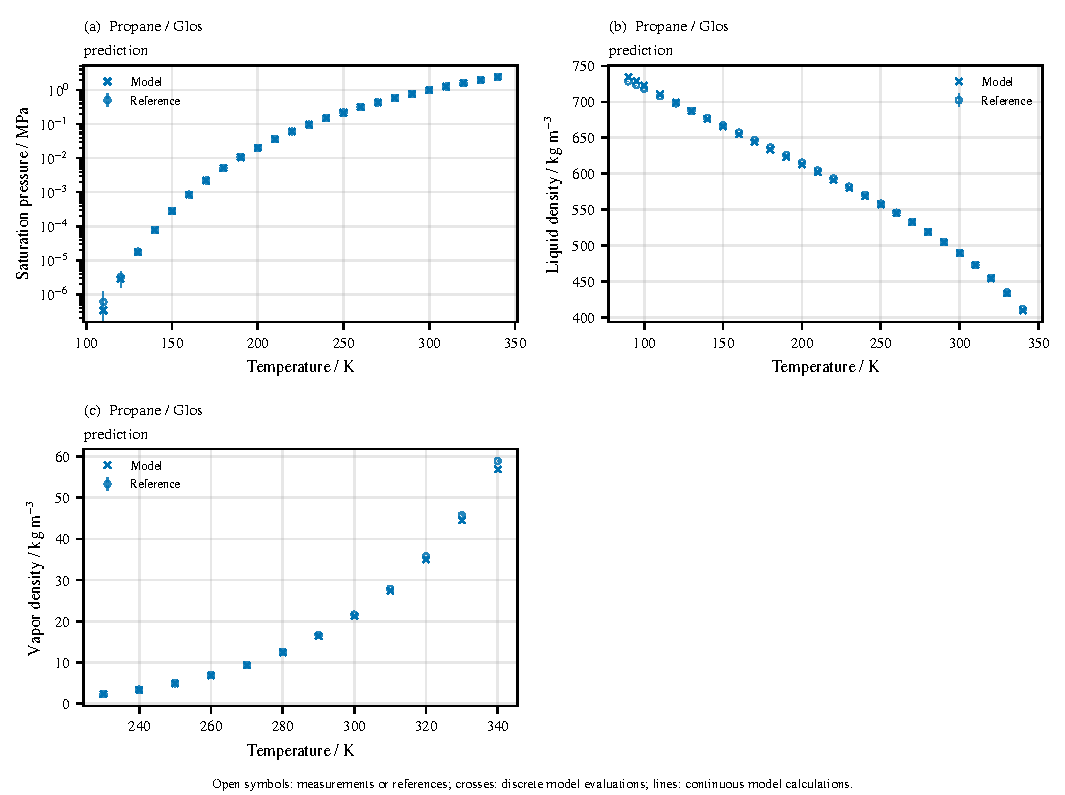
\includegraphics[page=1,width=\linewidth,height=19cm,keepaspectratio]{F8-pure-fluids}
\caption{Propane saturation pressure, saturated-liquid density and saturated-vapor density with the Gross--Sadowski parameters against the measurements of Glos et al., 90--340~K, with expanded measurement uncertainties (prediction)~\citep{Gross2001,Glos2004}.}
\label{fig:si-F8-pure-fluids-1}
\end{figure}
\clearpage

\begin{figure}[pos=p]
\centering
\includegraphics[page=2,width=\linewidth,height=19cm,keepaspectratio]{F8-pure-fluids}
\caption{Saturation pressures calculated for each of the 78 compounds of Gross and Sadowski; no measured reference is compared (numerical verification)~\citep{Gross2001}.}
\label{fig:si-F8-pure-fluids-2}
\end{figure}
\clearpage

\begin{figure}[pos=p]
\centering
\includegraphics[page=3,width=\linewidth,height=19cm,keepaspectratio]{F8-pure-fluids}
\caption{Saturated-liquid densities of diethyl ether, methane, propylene and toluene against measurements and digitized source-model values; diamonds mark the coldest states, where pressure closure failed~\citep{Gross2001}.}
\label{fig:si-F8-pure-fluids-3}
\end{figure}
\clearpage



\begin{figure}[pos=p]
\centering
\includegraphics[page=6,width=\linewidth,height=19cm,keepaspectratio]{F8-pure-fluids}
\caption{Saturation pressures of carbon dioxide, 220--300~K, and benzene, 290--540~K, with the quadrupolar parameters of Gross against the Span--Wagner reference equation and a DIPPR-101-form correlation; carbon dioxide also with nonpolar parameters (published-model reproduction)~\citep{grossEquationofstateContributionPolar2005,spanNewEquationState1996}.}
\label{fig:si-F8-pure-fluids-5}
\end{figure}
\clearpage

\begin{figure}[pos=p]
\centering
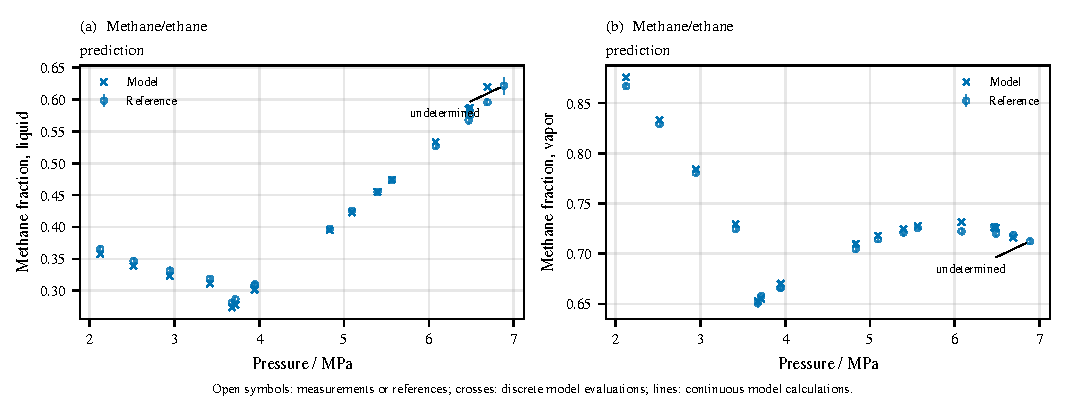
\includegraphics[page=1,width=\linewidth,height=19cm,keepaspectratio]{F9-neutral-mixtures}
\caption{Methane/ethane liquid and vapor methane fractions against the measurements of May et al., 203--244~K and 2.1--6.9~MPa, predicted with the Gross--Sadowski parameters and $k_{ij}=0$; one state is unavailable (prediction)~\citep{May2015,Gross2001}.}
\label{fig:si-F9-neutral-mixtures-1}
\end{figure}
\clearpage



\begin{figure}[pos=p]
\centering
\includegraphics[page=3,width=\linewidth,height=19cm,keepaspectratio]{F9-neutral-mixtures}
\caption{Liquid carbon dioxide fraction of carbon dioxide/THF at 313.2--353.2~K against the measurements and published model values of Schick et al.~\citep{Schick2023}.}
\label{fig:si-F9-neutral-mixtures-3}
\end{figure}
\clearpage

\begin{figure}[pos=p]
\centering
\includegraphics[page=4,width=\linewidth,height=19cm,keepaspectratio]{F9-neutral-mixtures}
\caption{Gross--Sadowski binary systems with the source's binary interactions: methane/butane, ethane/decane, ethane/diethyl ether, propane/benzene, carbon dioxide/decane, carbon dioxide/cyclohexane and hexane/1-chlorobutane, against measurements and digitized source-model values~\citep{Gross2001}.}
\label{fig:si-F9-neutral-mixtures-4}
\end{figure}
\clearpage

\begin{figure}[pos=p]
\centering
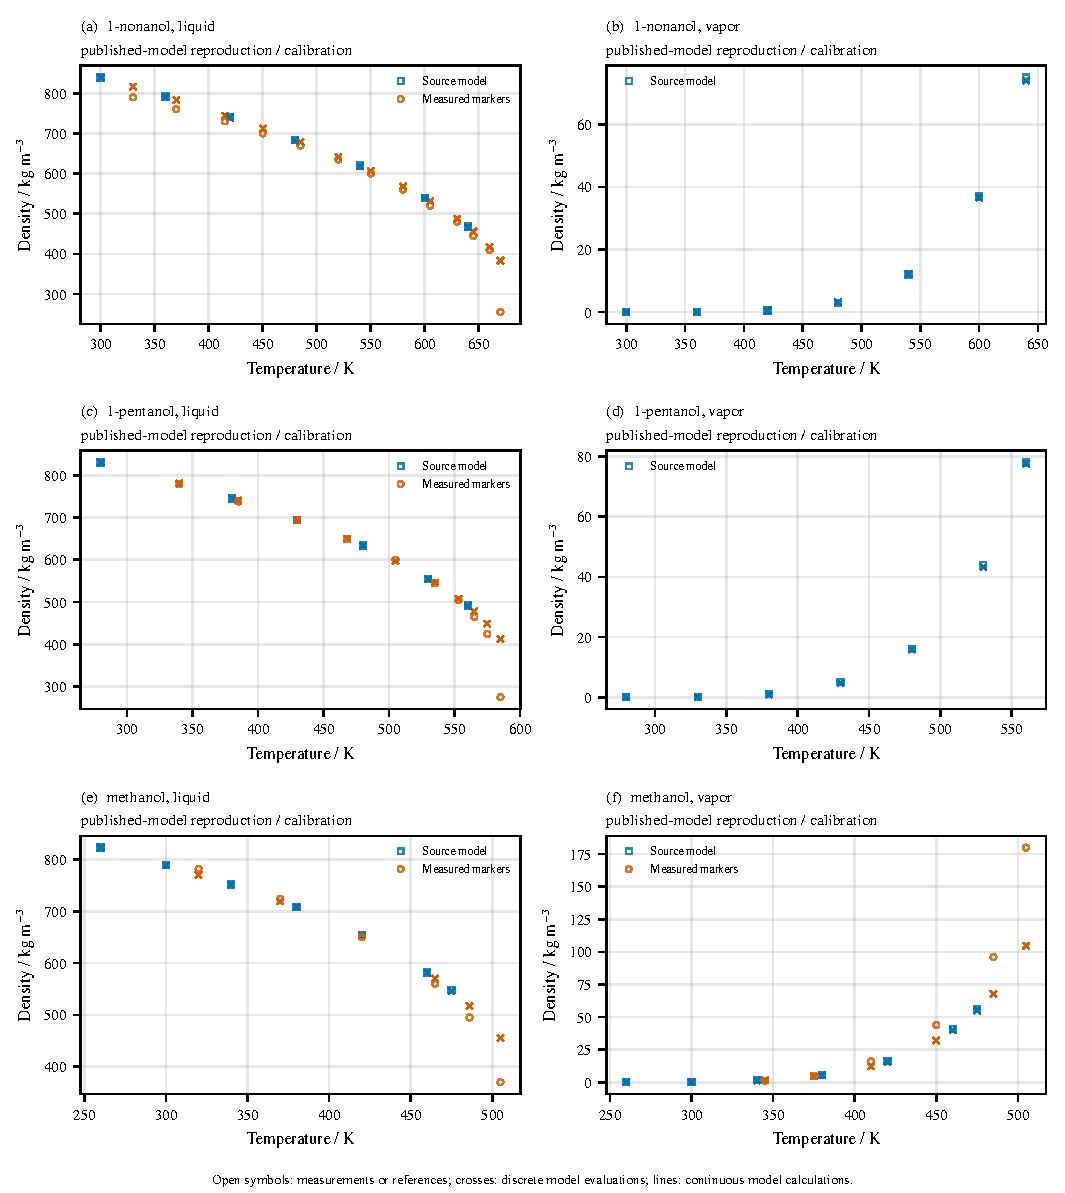
\includegraphics[page=1,width=\linewidth,height=19cm,keepaspectratio]{F10-associating}
\caption{Saturated-liquid and saturated-vapor densities of 1-nonanol, 1-pentanol and methanol with the Gross--Sadowski associating parameters, against measurements and digitized source-model values~\citep{Gross2002}.}
\label{fig:si-F10-associating-1}
\end{figure}
\clearpage

\begin{figure}[pos=p]
\centering
\includegraphics[page=2,width=\linewidth,height=19cm,keepaspectratio]{F10-associating}
\caption{Associating binary systems with the Gross--Sadowski parameters: isobutane/methanol, 1-propanol/ethylbenzene, 1-pentanol/benzene, 1-propanol/benzene, 2-propanol/benzene, butane/1-butanol, butane/ethanol, methanol/cyclohexane and methanol/1-octanol~\citep{Gross2002}.}
\label{fig:si-F10-associating-2}
\end{figure}
\clearpage





\begin{figure}[pos=p]
\centering
\includegraphics[page=2,width=\linewidth,height=19cm,keepaspectratio]{F11-aqueous-electrolytes}
\caption{Held et al.\ aqueous salt series, page 1 of five: solution density differences, vapor pressures, water activities and mean ionic activity coefficients of the 19 salts at 293.15--333.15~K, each against measurements and the digitized source-model curve; bars are the reading intervals of digitized values~\citep{Held2008}.}
\label{fig:si-F11-aqueous-electrolytes-2}
\end{figure}
\clearpage

\begin{figure}[pos=p]
\centering
\includegraphics[page=3,width=\linewidth,height=19cm,keepaspectratio]{F11-aqueous-electrolytes}
\caption{Held et al.\ aqueous salt series, page 2 of five: solution density differences, vapor pressures, water activities and mean ionic activity coefficients of the 19 salts at 293.15--333.15~K, each against measurements and the digitized source-model curve; bars are the reading intervals of digitized values~\citep{Held2008}.}
\label{fig:si-F11-aqueous-electrolytes-3}
\end{figure}
\clearpage

\begin{figure}[pos=p]
\centering
\includegraphics[page=4,width=\linewidth,height=19cm,keepaspectratio]{F11-aqueous-electrolytes}
\caption{Held et al.\ aqueous salt series, page 3 of five: solution density differences, vapor pressures, water activities and mean ionic activity coefficients of the 19 salts at 293.15--333.15~K, each against measurements and the digitized source-model curve; bars are the reading intervals of digitized values~\citep{Held2008}.}
\label{fig:si-F11-aqueous-electrolytes-4}
\end{figure}
\clearpage

\begin{figure}[pos=p]
\centering
\includegraphics[page=5,width=\linewidth,height=19cm,keepaspectratio]{F11-aqueous-electrolytes}
\caption{Held et al.\ aqueous salt series, page 4 of five: solution density differences, vapor pressures, water activities and mean ionic activity coefficients of the 19 salts at 293.15--333.15~K, each against measurements and the digitized source-model curve; bars are the reading intervals of digitized values~\citep{Held2008}.}
\label{fig:si-F11-aqueous-electrolytes-5}
\end{figure}
\clearpage

\begin{figure}[pos=p]
\centering
\includegraphics[page=6,width=\linewidth,height=19cm,keepaspectratio]{F11-aqueous-electrolytes}
\caption{Held et al.\ aqueous salt series, page 5 of five: solution density differences, vapor pressures, water activities and mean ionic activity coefficients of the 19 salts at 293.15--333.15~K, each against measurements and the digitized source-model curve; bars are the reading intervals of digitized values~\citep{Held2008}.}
\label{fig:si-F11-aqueous-electrolytes-6}
\end{figure}
\clearpage

\begin{figure}[pos=p]
\centering
\includegraphics[page=7,width=\linewidth,height=19cm,keepaspectratio]{F11-aqueous-electrolytes}
\caption{Practical osmotic coefficients with the Held 2014 parameters: NaCl, KCl and KBr at 298.15~K under both parameter strategies, and NaCl and KCl at 273.15~K, against the source-model curves and measurements~\citep{Held2014}.}
\label{fig:si-F11-aqueous-electrolytes-7}
\end{figure}
\clearpage

\begin{figure}[pos=p]
\centering
\includegraphics[page=8,width=\linewidth,height=19cm,keepaspectratio]{F11-aqueous-electrolytes}
\caption{Aqueous NaCl at 298.15~K: mean ionic activity coefficients fitted at or below 2~mol/kg and predicted above it, and relative permittivity. F0, published Figiel parameters with ion suppression; F1, D1 and P1, refits with the ion-suppression, density--temperature and dipolar-perturbation relations~\citep{Figiel2025,Yang2024,Rueben2024}.}
\label{fig:si-F11-aqueous-electrolytes-8}
\end{figure}
\clearpage











\begin{figure}[pos=p]
\centering
\includegraphics[page=2,width=\linewidth,height=19cm,keepaspectratio]{F4-phase-envelope}
\caption{Discrete comparisons of methane/ethane critical points and bubble and dew points with FeOs and teqp at their own compositions (numerical verification).}
\label{fig:si-F4-phase-envelope-2}
\end{figure}
\clearpage

\begin{figure}[pos=p]
\centering
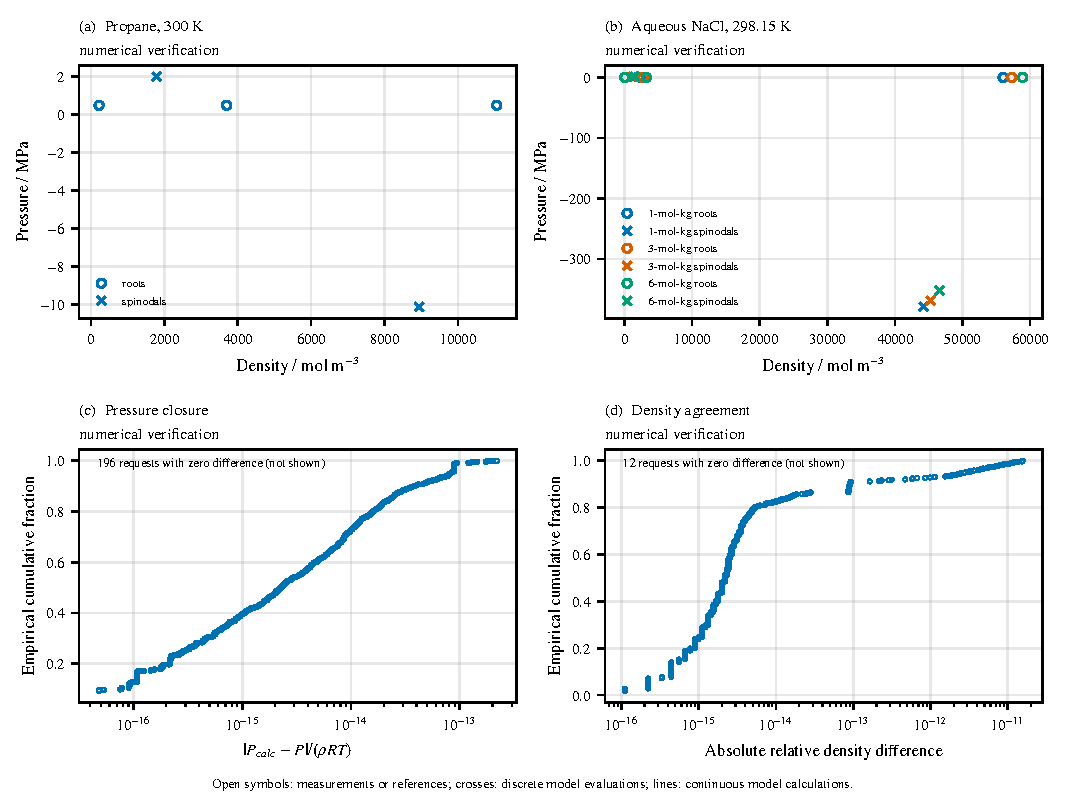
\includegraphics[page=1,width=\linewidth,height=19cm,keepaspectratio]{F2-density-roots}
\caption{Density roots and pressure closure (numerical verification). Top: roots and spinodals found for propane at 300~K and 0.499~MPa and for aqueous NaCl at 298.15~K and 0.1~MPa at 1, 3 and 6~mol/kg. Bottom: cumulative distributions of the reduced pressure residual and of the relative density difference from the frozen reference over the benchmark requests; requests with zero difference cannot be drawn on the logarithmic axis and are counted on each panel.}
\label{fig:si-F2-density-roots-1}
\end{figure}
\clearpage


\end{document}
